\chapter{Religious Melancholy}
{
%SECT. IV. MEMB. I.

%SUBSECT. I.-_Religious Melancholy. Its object God; what his beauty is; How it allures. The parts and parties affected_.
\section[Religious Melancholy, its object God]{Religious Melancholy. Its object God; what his beauty is; How it allures. The parts and parties affected.}

\lettrine{T}{hat} there is such a distinct species of love melancholy, no man hath
ever yet doubted: but whether this subdivision of \authorfootnote{6302}Religious
Melancholy be warrantable, it may be controverted.
\authorfootnote{6303}Pergite Pieridies, medio nec calle vagantem
Linquite me, qua nulla pedum vestigia ducunt,
Nulla rotae currus testantur signa priores.

I have no pattern to follow as in some of the rest, no man to imitate.
No physician hath as yet distinctly written of it as of the other; all
acknowledge it a most notable symptom, some a cause, but few a species
or kind. \authorfootnote{6304}Areteus, Alexander, Rhasis, Avicenna, and most of our
late writers, as Gordonius, Fuchsius, Plater, Bruel, Montaltus, \&c.
repeat it as a symptom. \authorfootnote{6305}Some seem to be inspired of the Holy
Ghost, some take upon them to be prophets, some are addicted to new
opinions, some foretell strange things, de statu mundi et Antichristi,
saith Gordonius. Some will prophesy of the end of the world to a day
almost, and the fall of the Antichrist, as they have been addicted or
brought up; for so melancholy works with them, as \authorfootnote{6306}Laurentius
holds. If they have been precisely given, all their meditations tend
that way, and in conclusion produce strange effects, the humour
imprints symptoms according to their several inclinations and
conditions, which makes \authorfootnote{6307}Guianerius and \authorfootnote{6308}Felix Plater put too
much devotion, blind zeal, fear of eternal punishment, and that last
judgment for a cause of those enthusiastics and desperate persons: but
some do not obscurely make a distinct species of it, dividing love
melancholy into that whose object is women; and into the other whose
object is God. Plato, in Convivio, makes mention of two distinct
furies; and amongst our neoterics, Hercules de Saxonia lib. 1. pract.
med. cap. 16. cap. de Melanch. doth expressly treat of it in a distinct
species. \authorfootnote{6309} Love melancholy (saith he) is twofold; the first is
that (to which peradventure some will not vouchsafe this name or
species of melancholy) affection of those which put God for their
object, and are altogether about prayer, fasting, \&c., the other about
women. Peter Forestus in his observations delivereth as much in the
same words: and Felix Platerus de mentis alienat. cap. 3.
frequentissima est ejus species, in qua curanda saepissime multum fui
impeditus; 'tis a frequent disease; and they have a ground of what they
say, forth of Areteus and Plato. \authorfootnote{6310}Areteus, an old author, in his
third book cap. 6. doth so divide love melancholy, and derives this
second from the first, which comes by inspiration or otherwise.
\authorfootnote{6311}Plato in his Phaedrus hath these words, Apollo's priests in
Delphos, and at Dodona, in their fury do many pretty feats, and benefit
the Greeks, but never in their right wits. He makes them all mad, as
well he might; and he that shall but consider that superstition of old,
those prodigious effects of it (as in its place I will shew the several
furies of our fatidici dii, pythonissas, sibyls, enthusiasts,
pseudoprophets, heretics, and schismatics in these our latter ages)
shall instantly confess, that all the world again cannot afford so much
matter of madness, so many stupendous symptoms, as superstition,
heresy, schism have brought out: that this species alone may be
paralleled to all the former, has a greater latitude, and more
miraculous effects; that it more besots and infatuates men, than any
other above named whatsoever, does more harm, works more disquietness
to mankind, and has more crucified the souls of mortal men (such hath
been the devil's craft) than wars, plagues, sicknesses, dearth, famine,
and all the rest.
Give me but a little leave, and I will set before your eyes in brief a
stupendous, vast, infinite ocean of incredible madness and folly: a sea
full of shelves and rocks, sands, gulfs, euripes and contrary tides,
full of fearful monsters, uncouth shapes, roaring waves, tempests, and
siren calms, halcyonian seas, unspeakable misery, such comedies and
tragedies, such absurd and ridiculous, feral and lamentable fits, that
I know not whether they are more to be pitied or derided, or may be
believed, but that we daily see the same still practised in our days,
fresh examples, nova novitia, fresh objects of misery and madness, in
this kind that are still represented unto us, abroad, at home, in the
midst of us, in our bosoms.
But before I can come to treat of these several errors and obliquities,
their causes, symptoms, affections, \&c., I must say something
necessarily of the object of this love, God himself, what this love is,
how it allureth, whence it proceeds, and (which is the cause of all our
miseries) how we mistake, wander and swerve from it.
Amongst all those divine attributes that God doth vindicate to himself,
eternity, omnipotency, immutability, wisdom, majesty, justice, mercy,
\&c., his \authorfootnote{6312}beauty is not the least, one thing, saith David, have I
desired of the Lord, and that I will still desire, to behold the beauty
of the Lord, Psal. xxvii. 4. And out of Sion, which is the perfection
of beauty, hath God shined, Psal. 1. 2. All other creatures are fair, I
confess, and many other objects do much enamour us, a fair house, a
fair horse, a comely person. \authorfootnote{6313}I am amazed, saith Austin, when 1
look up to heaven and behold the beauty of the stars, the beauty of
angels, principalities, powers, who can express it? who can
sufficiently commend, or set out this beauty which appears in us? so
fair a body, so fair a face, eyes, nose, cheeks, chin, brows, all fair
and lovely to behold; besides the beauty of the soul which cannot be
discerned. If we so labour and be so much affected with the comeliness
of creatures, how should we be ravished with that admirable lustre of
God himself? If ordinary beauty have such a prerogative and power, and
what is amiable and fair, to draw the eyes and ears, hearts and
affections of all spectators unto it, to move, win, entice, allure: how
shall this divine form ravish our souls, which is the fountain and
quintessence of all beauty? Coelum pulchrum, sed pulchrior coeli
fabricator; if heaven be so fair, the sun so fair, how much fairer
shall he be, that made them fair? For by the greatness and beauty of
the creatures, proportionally, the maker of them is seen, Wisd. xiii.
5. If there be such pleasure in beholding a beautiful person alone, and
as a plausible sermon, he so much affect us, what shall this beauty of
God himself, that is infinitely fairer than all creatures, men, angels,
\&c. \authorfootnote{6314} Omnis pulchritudo florem, hominum, angelorum, et rerum
omnium pulcherrimarum ad Dei pulchritudinem collata, nox est et
tenebrae, all other beauties are night itself, mere darkness to this
our inexplicable, incomprehensible, unspeakable, eternal, infinite,
admirable and divine beauty. This lustre, pulchritudo omnium
pulcherrima. This beauty and \authorfootnote{6315} splendour of the divine Majesty, is
it that draws all creatures to it, to seek it, love, admire, and adore
it; and those heathens, pagans, philosophers, out of those relics they
have yet left of God's image, are so far forth incensed, as not only to
acknowledge a God; but, though after their own inventions, to stand in
admiration of his bounty, goodness, to adore and seek him; the
magnificence and structure of the world itself, and beauty of all his
creatures, his goodness, providence, protection, enforceth them to love
him, seek him, fear him, though a wrong way to adore him: but for us
that are Christians, regenerate, that are his adopted sons, illuminated
by his word, having the eyes of our hearts and understandings opened;
how fairly doth he offer and expose himself? Ambit nos Deus (Austin
saith) donis et forma sua, he woos us by his beauty, gifts, promises,
to come unto him; \authorfootnote{6316}the whole Scripture is a message, an
exhortation, a love letter to this purpose; to incite us, and invite
us, \authorfootnote{6317}God's epistle, as Gregory calls it, to his creatures. He sets
out his son and his church in that epithalamium or mystical song of
Solomon, to enamour us the more, comparing his head to fine gold, his
locks curled and black as a raven, Cant. iv. 5. his eyes like doves on
rivers of waters, washed with milk, his lips as lilies, drooping down
pure juice, his hands as rings of gold set with chrysolite: and his
church to a vineyard, a garden enclosed, a fountain of living waters,
an orchard of pomegranates, with sweet scents of saffron, spike,
calamus and cinnamon, and all the trees of incense, as the chief
spices, the fairest amongst women, no spot in her, \authorfootnote{6318}his sister,
his spouse, undefiled, the only daughter of her mother, dear unto her,
fair as the moon, pure as the sun, looking out as the morning; that by
these figures, that glass, these spiritual eyes of contemplation, we
might perceive some resemblance of his beauty, the love between his
church and him. And so in the xlv. Psalm this beauty of his church is
compared to a queen in a vesture of gold of Ophir, embroidered raiment
of needlework, that the king might take pleasure in her beauty. To
incense us further yet, \authorfootnote{6319}John, in his apocalypse, makes a
description of that heavenly Jerusalem, the beauty, of it, and in it
the maker of it; Likening it to a city of pure gold, like unto clear
glass, shining and garnished with all manner of precious stones, having
no need of sun or moon: for the lamb is the light of it, the glory of
God doth illuminate it: to give us to understand the infinite glory,
beauty and happiness of it. Not that it is no fairer than these
creatures to which it is compared, but that this vision of his, this
lustre of his divine majesty, cannot otherwise be expressed to our
apprehensions, no tongue can tell, no heart can conceive it, as Paul
saith. Moses himself, Exod. xxxiii. 18. when he desired to see God in
his glory, was answered that he might not endure it, no man could see
his face and live. Sensibile forte destruit sensum, a strong object
overcometh the sight, according to that axiom in philosophy: fulgorem
solis ferre non potes, multo magis creatoris; if thou canst not endure
the sunbeams, how canst thou endure that fulgor and brightness of him
that made the sun? The sun itself and all that we can imagine, are but
shadows of it, 'tis visio praecellens, as \authorfootnote{6320}Austin calls it, the
quintessence of beauty this, which far exceeds the beauty of heavens,
sun and moon, stars, angels, gold and silver, woods, fair fields, and
whatsoever is pleasant to behold. All those other beauties fail, vary,
are subject to corruption, to loathing; \authorfootnote{6321}But this is an immortal
vision, a divine beauty, an immortal love, an indefatigable love and
beauty, with sight of which we shall never be tired nor wearied, but
still the more we see the more we shall covet him. \authorfootnote{6322}For as one
saith, where this vision is, there is absolute beauty; and where is
that beauty, from the same fountain comes all pleasure and happiness;
neither can beauty, pleasure, happiness, be separated from his vision
or sight, or his vision, from beauty, pleasure, happiness. In this life
we have but a glimpse of this beauty and happiness: we shall hereafter,
as John saith, see him as he is: thine eyes, as Isaiah promiseth,
xxxiii. 17. shall behold the king in his glory, then shall we be
perfectly enamoured, have a full fruition of it, desire, \authorfootnote{6323}behold
and love him alone as the most amiable and fairest object, or summum
bonum, or chiefest good.
This likewise should we now have done, had not our will been corrupted;
and as we are enjoined to love God with all our heart, and all our
soul: for to that end were we born, to love this object, as
\authorfootnote{6324}Melancthon discourseth, and to enjoy it. And him our will would
have loved and sought alone as our summum bonum, or principal good, and
all other good things for God's sake: and nature, as she proceeded from
it, would have sought this fountain; but in this infirmity of human
nature this order is disturbed, our love is corrupt: and a man is like
that monster in \authorfootnote{6325}Plato, composed of a Scylla, a lion and a man; we
are carried away headlong with the torrent of our affections: the
world, and that infinite variety of pleasing objects in it, do so
allure and enamour us, that we cannot so much as look towards God, seek
him, or think on him as we should: we cannot, saith Austin, Rempub.
coelestem cogitare, we cannot contain ourselves from them, their
sweetness is so pleasing to us. Marriage, saith \authorfootnote{6326} Gualter, detains
many; a thing in itself laudable, good and necessary, but many,
deceived and carried away with the blind love of it, have quite laid
aside the love of God, and desire of his glory. Meat and drink hath
overcome as many, whilst they rather strive to please, satisfy their
guts and belly, than to serve God and nature. Some are so busied about
merchandise to get money, they lose their own souls, whilst covetously
carried, and with an insatiable desire of gain, they forget God; as
much we may say of honour, leagues, friendships, health, wealth, and
all other profits or pleasures in this life whatsoever. \authorfootnote{6327}In this
world there be so many beautiful objects, splendours and brightness of
gold, majesty of glory, assistance of friends, fair promises, smooth
words, victories, triumphs, and such an infinite company of pleasing
beauties to allure us, and draw us from God, that we cannot look after
him. And this is it which Christ himself, those prophets and apostles
so much thundered against, 1 John, xvii. 15, dehort us from; love not
the world, nor the things that are in the world: if any man love the
world, the love of the Father is not in him, 16. For all that is in the
world, as lust of the flesh, the lust of the eyes, and pride of life,
is not of the Father, but of the world: and the world passeth away and
the lust thereof; but he that fulfilleth the will of God abideth for
ever. No man, saith our Saviour, can serve two masters, but he must
love the one and hate the other, \&c., bonos vel malos mores, boni vel
mali faciunt amores, Austin well infers: and this is that which all the
fathers inculcate. He cannot (\authorfootnote{6328}Austin admonisheth) be God's
friend, that is delighted with the pleasures of the world: make clean
thine heart, purify thine heart; if thou wilt see this beauty, prepare
thyself for it. It is the eye of contemplation by which we must behold
it, the wing of meditation which lifts us up and rears our souls with
the motion of our hearts, and sweetness of contemplation: so saith
Gregory cited by \authorfootnote{6329}Bonaventure. And as \authorfootnote{6330}Philo Judeus seconds
him, he that loves God, will soar aloft and take him wings; and leaving
the earth fly up to heaven, wander with sun and moon, stars, and that
heavenly troop, God himself being his guide. If we desire to see him,
we must lay aside all vain objects, which detain us and dazzle our
eyes, and as \authorfootnote{6331}Ficinus adviseth us, get us solar eyes, spectacles
as they that look on the sun: to see this divine beauty, lay aside all
material objects, all sense, and then thou shalt see him as he is. Thou
covetous wretch, as \authorfootnote{6332}Austin expostulates, why dost thou stand
gaping on this dross, muck-hills, filthy excrements? behold a far
fairer object, God himself woos thee; behold him, enjoy him, he is sick
for love. Cant. v. he invites thee to his sight, to come into his fair
garden, to eat and drink with him, to be merry with him, to enjoy his
presence for ever. \authorfootnote{6333}Wisdom cries out in the streets besides the
gates, in the top of high places, before the city, at the entry of the
door, and bids them give ear to her instruction, which is better than
gold or precious stones; no pleasures can be compared to it: leave all
then and follow her, vos exhortor o amici et obsecro. In.
\authorfootnote{6334}Ficinus's words, I exhort and beseech you, that you would embrace
and follow this divine love with all your hearts and abilities, by all
offices and endeavours make this so loving God propitious unto you. For
whom alone, saith \authorfootnote{6335}Plotinus, we must forsake the kingdoms and
empires of the whole earth, sea, land, and air, if we desire to be
engrafted into him, leave all and follow him.
Now, forasmuch as this love of God is a habit infused of God, as \authorfootnote{6336}
Thomas holds, l. 2. quaest. 23. by which a man is inclined to love God
above all, and his neighbour as himself, we must pray to God that he
will open our eyes, make clear our hearts, that we may be capable of
his glorious rays, and perform those duties that he requires of us,
Deut. vi. and Josh. xxiii. to love God above all, and our neighbour as
ourself, to keep his commandments. In this we know, saith John, c. v.
2, we love the children of God, when we love God and keep his
commandments. This is the love of God, that we keep his commandments;
he that loveth not, knoweth not God, for God is love, cap. iv. 8, and
he that dwelleth in love, dwelleth in God, and God in him; for love
pre-supposeth knowledge, faith, hope, and unites us to God himself, as
\authorfootnote{6337}Leon Hebreus delivereth unto us, and is accompanied with the fear
of God, humility, meekness, patience, all those virtues, and charity
itself. For if we love God, we shall love our neighbour, and perform
the duties which are required at our hands, to which we are exhorted, 1
Cor. xv. 4, 5; Ephes. iv.; Colos. iii.; Rom. xii. We shall not be
envious or puffed up, or boast, disdain, think evil, or be provoked to
anger, but suffer all things; endeavour to keep the unity of the spirit
in the bond of peace. Forbear one another, forgive one another, clothe
the naked, visit the sick, and perform all those works of mercy, which
\authorfootnote{6338}Clemens Alexandrinus calls amoris et amicitiae, impletionem et
extentionem, the extent and complement of love; and that not for fear
or worldly respects, but ordine ad Deum, for the love of God himself.
This we shall do if we be truly enamoured; but we come short in both,
we neither love God nor our neighbour as we should. Our love in
spiritual things is too \authorfootnote{6339}defective, in worldly things too
excessive, there is a jar in both. We love the world too much; God too
little; our neighbour not at all, or for our own ends. Vulgus amicitias
utilitate probat. The chief thing we respect is our commodity; and what
we do is for fear of worldly punishment, for vainglory, praise of men,
fashion, and such by respects, not for God's sake. We neither know God
aright, nor seek, love or worship him as we should. And for these
defects, we involve ourselves into a multitude of errors, we swerve
from this true love and worship of God: which is a cause unto us of
unspeakable miseries; running into both extremes, we become fools,
madmen, without sense, as now in the next place 1 will show you.
The parties affected are innumerable almost, and scattered over the
face of the earth, far and near, and so have been in all precedent
ages, from the beginning of the world to these times, of all sorts and
conditions. For method's sake I will reduce them to a twofold division,
according to those two extremes of excess and defect, impiety and
superstition, idolatry and atheism. Not that there is any excess of
divine worship or love of God; that cannot be, we cannot love God too
much, or do our duty as we ought, as Papists hold, or have any
perfection in this life, much less supererogate: when we have all done,
we are unprofitable servants. But because we do aliud agere, zealous
without knowledge, and too solicitous about that which is not
necessary, busying ourselves about impertinent, needless, idle, and
vain ceremonies, populo ut placerent, as the Jews did about sacrifices,
oblations, offerings, incense, new moons, feasts, \&c., but Isaiah
taxeth them, i. 12, who required this at your hands? We have too great
opinion of our own worth, that we can satisfy the law: and do more than
is required at our hands, by performing those evangelical counsels, and
such works of supererogation, merit for others, which Bellarmine,
Gregory de Valentia, all their Jesuits and champions defend, that if
God should deal in rigour with them, some of their Franciscans and
Dominicans are so pure, that nothing could be objected to them. Some of
us again are too dear, as we think, more divine and sanctified than
others, of a better mettle, greater gifts, and with that proud
Pharisee, contemn others in respect of ourselves, we are better
Christians, better learned, choice spirits, inspired, know more, have
special revelation, perceive God's secrets, and thereupon presume, say
and do that many times which is not befitting to be said or done. Of
this number are all superstitious idolaters, ethnics, Mahometans, Jews,
heretics, \authorfootnote{6340}enthusiasts, divinators, prophets, sectaries, and
schismatics. Zanchius reduceth such infidels to four chief sects; but I
will insist and follow mine own intended method: all which with many
other curious persons, monks, hermits, \&c., may be ranged in this
extreme, and fight under this superstitious banner, with those rude
idiots, and infinite swarms of people that are seduced by them. In the
other extreme or in defect, march those impious epicures, libertines,
atheists, hypocrites, infidels, worldly, secure, impenitent,
unthankful, and carnal-minded men, that attribute all to natural
causes, that will acknowledge no supreme power; that have cauterised
consciences, or live in a reprobate sense; or such desperate persons as
are too distrustful of his mercies. Of these there be many
subdivisions, diverse degrees of madness and folly, some more than
other, as shall be shown in the symptoms: and yet all miserably out,
perplexed, doting, and beside themselves for religion's sake. For as
\authorfootnote{6341}Zanchy well distinguished, and all the world knows religion is
twofold, true or false; false is that vain superstition of idolaters,
such as were of old, Greeks, Romans, present Mahometans, \&c. Timorem
deorum inanem, \authorfootnote{6342}Tully could term it; or as Zanchy defines it, Ubi
falsi dii, aut falso cullu colitur Deus, when false gods, or that God
is falsely worshipped. And 'tis a miserable plague, a torture of the
soul, a mere madness, Religiosa insania, \authorfootnote{6343}Meteran calls it, or
insanus error, as \authorfootnote{6344}Seneca, a frantic error; or as Austin, Insanus
animi morbus, a furious disease of the soul; insania omnium
insanissima, a quintessence of madness; \authorfootnote{6345}for he that is
superstitious can never be quiet. 'Tis proper to man alone, uni
superbia, avaritia, superstitio, saith Plin. lib. 7. cap. 1. atque
etiam post saevit de futuro, which wrings his soul for the present, and
to come: the greatest misery belongs to mankind, a perpetual servitude,
a slavery, \authorfootnote{6346}Ex timore timor, a heavy yoke, the seal of damnation,
an intolerable burden. They that are superstitious are still fearing,
suspecting, vexing themselves with auguries, prodigies, false tales,
dreams, idle, vain works, unprofitable labours, as \authorfootnote{6347}Boterus
observes, cura mentis ancipite versantur: enemies to God and to
themselves. In a word, as Seneca concludes, Religio Deum colit,
superstitio destruit, superstition destroys, but true religion honours
God. True religion, ubi verus Deus vere colitur, where the true God is
truly worshipped, is the way to heaven, the mother of virtues, love,
fear, devotion, obedience, knowledge, \&c. It rears the dejected soul of
man, and amidst so many cares, miseries, persecutions, which this world
affords, it is a sole ease, an unspeakable comfort, a sweet reposal,
Jugum suave, et leve, a light yoke, an anchor, and a haven. It adds
courage, boldness, and begets generous spirits: although tyrants rage,
persecute, and that bloody Lictor or sergeant be ready to martyr them,
aut lita, aut morere, (as in those persecutions of the primitive
Church, it was put in practice, as you may read in Eusebius and others)
though enemies be now ready to invade, and all in an uproar, \authorfootnote{6348}Si
fractus illabatur orbis, impavidos ferient ruinae, though heaven should
fall on his head, he would not be dismayed. But as a good Christian
prince once made answer to a menacing Turk, facile scelerata hominum
arma contemnit, qui del praesidio tutus est: or as \authorfootnote{6349} Phalaris writ
to Alexander in a wrong cause, he nor any other enemy could terrify
him, for that he trusted in God. Si Deus nobiscum, quis contra nos? In
all calamities, persecutions whatsoever, as David did, 2 Sam. ii. 22,
he will sing with him, the Lord is my rock, my fortress, my strength,
my refuge, the tower and horn of my salvation, \&c. In all troubles and
adversities, Psal. xlvi. 1. God is my hope and help, still ready to be
found, I will not therefore fear, \&c., 'tis a fear expelling fear; he
hath peace of conscience, and is full of hope, which is (saith
\authorfootnote{6350}Austin) vita vitae mortalis, the life of this our mortal life,
hope of immortality, the sole comfort of our misery: otherwise, as Paul
saith, we of all others were most wretched, but this makes us happy,
counterpoising our hearts in all miseries; superstition torments, and
is from the devil, the author of lies; but this is from God himself, as
Lucian, that Antiochian priest, made his divine confession in
\authorfootnote{6351}Eusebius, Auctor nobis de Deo Deus est, God is the author of our
religion himself, his word is our rule, a lantern to us, dictated by
the Holy Ghost, he plays upon our hearts as many harpstrings, and we
are his temples, he dwelleth in us, and we in him.
The part affected of superstition, is the brain, heart, will,
understanding, soul itself, and all the faculties of it, totum
compositum, all is mad and dotes: now for the extent, as I say, the
world itself is the subject of it, (to omit that grand sin of atheism,)
all times have been misaffected, past, present, there is not one that
doth good, no not one, from the prophet to the priest, \&c. A lamentable
thing it is to consider, how many myriads of men this idolatry and
superstition (for that comprehends all) hath infatuated in all ages,
besotted by this blind zeal, which is religion's ape, religion's
bastard, religion's shadow, false glass. For where God hath a temple,
the devil will have a chapel: where God hath sacrifices, the devil will
have his oblations: where God hath ceremonies, the devil will have his
traditions: where there is any religion, the devil will plant
superstition; and 'tis a pitiful sight to behold and read, what
tortures, miseries, it hath procured, what slaughter of souls it hath
made, how it rageth amongst those old Persians, Syrians, Egyptians,
Greeks, Romans, Tuscans, Gauls, Germans, Britons, \&c. Britannia jam
hodie celebrat tam attonite, saith \authorfootnote{6352}Pliny, tantis ceremoniis
(speaking of superstition) ut dedisse Persis videri possit. The Britons
are so stupendly superstitious in their ceremonies, that they go beyond
those Persians. He that shall but read in Pausanias alone, those gods,
temples, altars, idols, statues, so curiously made with such infinite
cost and charge, amongst those old Greeks, such multitudes of them and
frequent varieties, as \authorfootnote{6353}Gerbelius truly observes, may stand
amazed, and never enough wonder at it; and thank God withal, that by
the light of the Gospel, we are so happily freed from that slavish
idolatry in these our days. But heretofore, almost in all countries, in
all places, superstition hath blinded the hearts of men; in all ages
what a small portion hath the true church ever been! Divisum imperium
cum Jove Daemon habet. \authorfootnote{6354}The patriarchs and their families, the
Israelites a handful in respect, Christ and his apostles, and not all
of them, neither. Into what straits hath it been compinged, a little
flock! how hath superstition on the other side dilated herself, error,
ignorance, barbarism, folly, madness, deceived, triumphed, and insulted
over the most wise discreet, and understanding man, philosophers,
dynasts, monarchs, all were involved and overshadowed in this mist, in
more than Cimmerian darkness. \authorfootnote{6355}Adeo ignara superstitio mentes
hominum depravat, et nonnunquam sapientum animos transversos agit. At
this present, quota pars! How small a part is truly religious! How
little in respect! Divide the world into six parts, and one, or not so
much, as Christians; idolaters and Mahometans possess almost Asia,
Africa, America, Magellanica. The kings of China, great Cham, Siam, and
Borneo, Pegu, Deccan, Narsinga, Japan, \&c., are gentiles, idolaters,
and many other petty princes in Asia, Monomotopa, Congo, and I know not
how many Negro princes in Africa, all Terra Australis incognita most of
America pagans, differing all in their several superstitions; and yet
all idolaters. The Mahometans extend themselves over the great Turk's
dominions in Europe, Africa, Asia, to the Xeriffes in Barbary, and its
territories in Fez, Sus, Morocco, \&c. The Tartar, the great Mogor, the
Sophy of Persia, with most of their dominions and subjects, are at this
day Mahometans. See how the devil rageth: those at odds, or differing
among themselves, some for \authorfootnote{6356}Ali, some Enbocar, for Acmor, and
Ozimen, those four doctors, Mahomet's successors, and are subdivided
into seventy-two inferior sects, as \authorfootnote{6357}Leo Afer reports. The Jews,
as a company of vagabonds, are scattered over all parts; whose story,
present estate, progress from time to time, is fully set down by
\authorfootnote{6358}Mr. Thomas Jackson, Doctor of Divinity, in his comment on the
creed. A fifth part of the world, and hardly that, now professeth
CHRIST, but so inlarded and interlaced with several superstitions, that
there is scarce a sound part to be found, or any agreement amongst
them. Presbyter John, in Africa, lord of those Abyssinians, or
Ethiopians, is by his profession a Christian, but so different from us,
with such new absurdities and ceremonies, such liberty, such a mixture
of idolatry and paganism, \authorfootnote{6359}that they keep little more than a bare
title of Christianity. They suffer polygamy, circumcision, stupend
fastings, divorce as they will themselves, \&c., and as the papists call
on the Virgin Mary, so do they on Thomas Didymus before Christ.
\authorfootnote{6360}The Greek or Eastern Church is rent from this of the West, and as
they have four chief patriarchs, so have they four subdivisions,
besides those Nestorians, Jacobins, Syrians, Armenians, Georgians, \&c.,
scattered over Asia Minor, Syria, Egypt, \&c., Greece, Walachia,
Circassia, Bulgaria, Bosnia, Albania, Illyricum, Sclavonia, Croatia,
Thrace, Servia, Rascia, and a sprinkling amongst the Tartars, the
Russians, Muscovites, and most of that great duke's (czar's) subjects,
are part of the Greek Church, and still Christians: but as \authorfootnote{6361}one
saith, temporis successu multas illi addiderunt superstitiones. In
process of time they have added so many superstitions, they be rather
semi-Christians than otherwise. That which remains is the Western
Church with us in Europe, but so eclipsed with several schisms,
heresies and superstitions, that one knows not where to find it. The
papists have Italy, Spain, Savoy, part of Germany, France, Poland, and
a sprinkling in the rest of Europe. In America, they hold all that
which Spaniards inhabit, Hispania Nova, Castella Aurea, Peru, \&c. In
the East Indies, the Philippines, some small holds about Goa, Malacca,
Zelan, Ormus, \&c., which the Portuguese got not long since, and those
land-leaping Jesuits have essayed in China, Japan, as appears by their
yearly letters; in Africa they have Melinda, Quiloa, Mombaze, \&c., and
some few towns, they drive out one superstition with another. Poland is
a receptacle of all religions, where Samosetans, Socinians, Photinians
(now protected in Transylvania and Poland), Arians, Anabaptists are to
be found, as well as in some German cities. Scandia is Christian, but
\authorfootnote{6362}Damianus A-Goes, the Portugal knight, complains, so mixed with
magic, pagan rites and ceremonies, they may be as well counted
idolaters: what Tacitus formerly said of a like nation, is verified in
them, \authorfootnote{6363}A people subject to superstition, contrary to religion. And
some of them as about Lapland and the Pilapians, the devil's possession
to this day, Misera haec gens (saith mine \authorfootnote{6364}author) Satanae
hactenus possessio,-et quod maxime mirandum et dolendum, and which is
to be admired and pitied; if any of them be baptised, which the kings
of Sweden much labour, they die within seven or nine days after, and
for that cause they will hardly be brought to Christianity, but worship
still the devil, who daily appears to them. In their idolatrous
courses, Gandentibus diis patriis, quos religiose colunt, \&c. Yet are
they very superstitious, like our wild Irish: though they of the better
note, the kings of Denmark and Sweden themselves, that govern them, be
Lutherans; the remnant are Calvinists, Lutherans, in Germany equally
mixed. And yet the emperor himself, dukes of Lorraine, Bavaria, and the
princes, electors, are most part professed papists. And though some
part of France and Ireland, Great Britain, half the cantons in
Switzerland, and the Low Countries, be Calvinists, more defecate than
the rest, yet at odds amongst themselves, not free from superstition.
And which \authorfootnote{6365}Brochard, the monk, in his description of the Holy
Land, after he had censured the Greek church, and showed their errors,
concluded at last, Faxit Deus ne Latinis multa irrepserint stultifies,
I say God grant there be no fopperies in our church. As a dam of water
stopped in one place breaks out into another, so doth superstition. I
say nothing of Anabaptists, Socinians, Brownists, Familists, \&c. There
is superstition in our prayers, often in our hearing of sermons, bitter
contentions, invectives, persecutions, strange conceits, besides
diversity of opinions, schisms, factions, \&c. But as the Lord (Job
xlii. cap. 7. v.) said to Eliphaz, the Temanite, and his two friends,
his wrath was kindled against them, for they had not spoken of him
things that were right: we may justly of these schismatics and
heretics, how wise soever in their own conceits, non recte loquuntur de
Deo, they speak not, they think not, they write not well of God, and as
they ought. And therefore, Quid quaeso mi Dorpi, as Erasmus concludes
to Dorpius, hisce Theologis faciamus, aut quid preceris, nisi forte
fidelem medicum, qui cerebro medeatur? What shall we wish them, but
sanam mentem, and a good physician? But more of their differences,
paradoxes, opinions, mad pranks, in the symptoms: I now hasten to the
causes.

%SUBSECT. II.-_Causes of Religious melancholy. From the Devil by miracles, apparitions, oracles. His instruments or factors, politicians, Priests, Impostors, Heretics, blind guides. In them simplicity, fear, blind zeal, ignorance, solitariness, curiosity, pride, vainglory, presumption, \&c. his engines, fasting, solitariness, hope, fear, \&c._
\section[Causes of Religious melancholy]{Causes of Religious melancholy. From the Devil by miracles, apparitions, oracles. His instruments or factors, politicians, Priests, Impostors, Heretics, blind guides. In them simplicity, fear, blind zeal, ignorance, solitariness, curiosity, pride, vainglory, presumption, \&c. his engines, fasting, solitariness, hope, fear, \&c.}

\lettrine{W}{e} are taught in Holy Scripture, that the Devil rangeth abroad like a
roaring lion, still seeking whom he may devour: and as in several
shapes, so by several engines and devices he goeth about to seduce us;
sometimes he transforms himself into an angel of light; and is so
cunning that he is able, if it were possible, to deceive the very
elect. He will be worshipped as \authorfootnote{6366}God himself, and is so adored by
the heathen, and esteemed. And in imitation of that divine power, as
\authorfootnote{6367}Eusebius observes, \authorfootnote{6368}to abuse or emulate God's glory, as
Dandinus adds, he will have all homage, sacrifices, oblations, and
whatsoever else belongs to the worship of God, to be done likewise unto
him, similis erit altissimo, and by this means infatuates the world,
deludes, entraps, and destroys many a thousand souls. Sometimes by
dreams, visions (as God to Moses by familiar conference), the devil in
several shapes talks with them: in the \authorfootnote{6369}Indies it is common, and
in China nothing so familiar as apparitions, inspirations, oracles, by
terrifying them with false prodigies, counterfeit miracles, sending
storms, tempests, diseases, plagues (as of old in Athens there was
Apollo, Alexicacus, Apollo λόιμιος, pestifer et malorum depulsor),
raising wars, seditions by spectrums, troubling their consciences,
driving them to despair, terrors of mind, intolerable pains; by
promises, rewards, benefits, and fair means, he raiseth such an opinion
of his deity and greatness, that they dare not do otherwise than adore
him, do as he will have them, they dare not offend him. And to compel
them more to stand in awe of him, \authorfootnote{6370}he sends and cures diseases,
disquiets their spirits (as Cyprian saith), torments and terrifies
their souls, to make them adore him: and all his study, all his
endeavour is to divert them from true religion to superstition: and
because he is damned himself, and in an error, he would have all the
world participate of his errors, and be damned with him. The primum
mobile, therefore, and first mover of all superstition, is the devil,
that great enemy of mankind, the principal agent, who in a thousand
several, shapes, after diverse fashions, with several engines,
illusions, and by several names hath deceived the inhabitants of the
earth, in several places and countries, still rejoicing at their falls.
All the world over before Christ's time, he freely domineered, and held
the souls of men in most slavish subjection (saith \authorfootnote{6371}Eusebius) in
diverse forms, ceremonies, and sacrifices, till Christ's coming, as if
those devils of the air had shared the earth amongst them, which the
Platonists held for gods (\authorfootnote{6372}Ludus deorum sumus), and were our
governors and keepers. In several places, they had several rites,
orders, names, of which read Wierus de praestigiis daemonum, lib. 1.
cap. 5. \authorfootnote{6373}Strozzius Cicogna, and others; Adonided amongst the
Syrians; Adramalech amongst the Capernaites, Asiniae amongst the
Emathites; Astartes with the Sidonians; Astaroth with the Palestines;
Dagon with the Philistines; Tartary with the Hanaei; Melchonis amongst
the Ammonites: Beli the Babylonians; Beelzebub and Baal with the
Samaritans and Moabites; Apis, Isis, and Osiris amongst the Egyptians;
Apollo Pythius at Delphos, Colophon, Ancyra, Cuma, Erythra; Jupiter in
Crete, Venus at Cyprus, Juno at Carthage, Aesculapius at Epidaurus,
Diana at Ephesus, Pallas at Athens, \&c. And even in these our days,
both in the East and West Indies, in Tartary, China, Japan, \&c., what
strange idols, in what prodigious forms, with what absurd ceremonies
are they adored? What strange sacraments, like ours of Baptism and the
Lord's Supper, what goodly temples, priests, sacrifices they had in
America, when the Spaniards first landed there, let Acosta the Jesuit
relate, lib. 5. cap. 1, 2, 3, 4, \&c., and how the devil imitated the
Ark and the children of Israel's coming out of Egypt; with many such.
For as Lipsius well discourseth out of the doctrine of the Stoics,
maxime cupiunt adorationem hominum, now and of old, they still and most
especially desire to be adored by men. See but what Vertomannus, l. 5.
c. 2. Marcus Polus, Lerius, Benzo, P. Martyr in his Ocean Decades,
Acosta, and Mat. Riccius expedit. Christ. in Sinus, lib. 1. relate.
\authorfootnote{6374}Eusebius wonders how that wise city of Athens, and flourishing
kingdoms of Greece, should be so besotted; and we in our times, how.
those witty Chinese, so perspicacious in all other things should be so
gulled, so tortured with superstition, so blind as to worship stocks
and stones. But it is no marvel, when we see all out as great effects
amongst Christians themselves; how are those Anabaptists, Arians, and
Papists above the rest, miserably infatuated! Mars, Jupiter, Apollo,
and Aesculapius, have resigned their interest, names, and offices to
Saint George.
(\authorfootnote{6375}(Maxime bellorum rector, quem nostra juventus
Pro Mavorte colit.)---

St. Christopher, and a company of fictitious saints, Venus to the Lady
of Loretto. And as those old Romans had several distinct gods, for
divers offices, persons, places, so have they saints, as \authorfootnote{6376}Lavater
well observes out of Lactantius, mutato nomine tantum, 'tis the same
spirit or devil that deludes them still. The manner how, as I say, is
by rewards, promises, terrors, affrights, punishments. In a word, fair
and foul means, hope and fear. How often hath Jupiter, Apollo, Bacchus,
and the rest, sent plagues in \authorfootnote{6377}Greece and Italy, because their
sacrifices were neglected?
\authorfootnote{6378}Dii multa neglecti dederunt
Hesperiae mala luctuosae,

to terrify them, to arouse them up, and the like: see but Livy,
Dionysius Halicarnassaeus, Thucydides, Pausanius, Philostratus,
\authorfootnote{6379}Polybius, before the battle of Cannae, prodigiis signis,
ostentis, templa cuncta, privates etiam aedes scatebant. Oeneus reigned
in Aetolia, and because he did not sacrifice to Diana with his other
gods (see more in Labanius his Diana), she sent a wild boar, insolitae
magnitudinis, qui terras et homines misere depascebatur, to spoil both
men and country, which was afterwards killed by Meleager. So Plutarch
in the Life of Lucullus relates, how Mithridates, king of Pontus, at
the siege of Cizicum, with all his navy, was overthrown by Proserpina,
for neglecting of her holy day. She appeared in a vision to Aristagoras
in the night, Cras inquit tybicinem Lybicum cum tybicine pontico
committam (tomorrow I will cause a contest between a Libyan and a
Pontic minstrel), and the day following this enigma was understood; for
with a great south wind which came from Libya, she quite overwhelmed
Mithridates' army. What prodigies and miracles, dreams, visions,
predictions, apparitions, oracles, have been of old at Delphos, Dodona,
Trophonius' den, at Thebes, and Lebaudia, of Jupiter Ammon in Egypt,
Amphiaraus in Attica, \&c.; what strange cures performed by Apollo and
Aesculapius? Juno's image and that of \authorfootnote{6380}Fortune spake, \authorfootnote{6381}Castor
and Pollux fought in person for the Romans against Hannibal's army, as
Pallas, Mars, Juno, Venus, for Greeks and Trojans, \&c. Amongst our
pseudo-Catholics nothing so familiar as such miracles; how many cures
done by our lady of Loretto, at Sichem! of old at our St. Thomas's
shrine, \&c. \authorfootnote{6382}St. Sabine was seen to fight for Arnulphus, duke of
Spoleto. \authorfootnote{6383}St. George fought in person for John the Bastard of
Portugal, against the Castilians; St. James for the Spaniards in
America. In the battle of Bannockburn, where Edward the Second, our
English king, was foiled by the Scots, St. Philanus' arm was seen to
fight (if \authorfootnote{6384}Hector Boethius doth not impose), that was before shut
up in a silver cap-case; another time, in the same author, St. Magnus
fought for them. Now for visions, revelations, miracles, not only out
of the legend, out of purgatory, but everyday comes news from the
Indies, and at home read the Jesuits' Letters, Ribadineira,
Thurselinus, Acosta, Lippomanus, Xaverius, Ignatius' Lives, \&c., and
tell me what difference?
His ordinary instruments or factors which he useth, as God himself, did
good kings, lawful magistrates, patriarchs, prophets, to the
establishing of his church, \authorfootnote{6385}are politicians, statesmen, priests,
heretics, blind guides, impostors, pseudoprophets, to propagate his
superstition. And first to begin of politicians, it hath ever been a
principal axiom with them to maintain religion or superstition, which
they determine of, alter and vary upon all occasions, as to them seems
best, they make religion mere policy, a cloak, a human invention, nihil
aeque valet ad regendos vulgi animos ac superstitio, as \authorfootnote{6386}Tacitus
and \authorfootnote{6387}Tully hold. Austin, l. 4. de civitat. Dei. c. 9. censures
Scaevola saying and acknowledging expedire civitates religione falli,
that it was a fit thing cities should be deceived by religion,
according to the diverb, Si mundus vult decipi, decipiatur, if the
world will be gulled, let it be gulled, 'tis good howsoever to keep it
in subjection. 'Tis that \authorfootnote{6388}Aristotle and \authorfootnote{6389}Plato inculcate in
their politics, Religion neglected, brings plague to the city, opens a
gap to all naughtiness. 'Tis that which all our late politicians
ingeminate. Cromerus, l. 2. pol. hist. Boterus, l. 3. de incrementis
urbium. Clapmarius, l. 2. c. 9. de Arcanis rerump. cap. 4. lib. 2.
polit. Captain Machiavel will have a prince by all means to counterfeit
religion, to be superstitious in show at least, to seem to be devout,
frequent holy exercises, honour divines, love the church, affect
priests, as Numa, Lycurgus, and such lawmakers were and did, non ut his
fidem habeant, sed ut subditos religionis metu facilius in officio
contineant, to keep people in obedience. \authorfootnote{6390}Nam naturaliter (as
Cardan writes) lex Christiana lex est pietatis, justitiae, fidei,
simplicitatis, \&c. But this error of his, Innocentius Jentilettus, a
French lawyer, theorem. 9. comment. 1. de Relig, and Thomas Bozius in
his book de ruinis gentium et Regnorum have copiously confuted. Many
politicians, I dare not deny, maintain religion as a true means, and
sincerely speak of it without hypocrisy, are truly zealous and
religious themselves. Justice and religion are the two chief props and
supporters of a well-governed commonwealth: but most of them are but
Machiavellians, counterfeits only for political ends; for solus rex
(which Campanella, cap. 18. atheismi triumphali observes), as amongst
our modern Turks, reipub. Finis, as knowing \authorfootnote{6391}magnus ejus in animos
imperium; and that, as \authorfootnote{6392}Sabellicus delivers, A man without
religion, is like a horse without a bridle. No way better to curb than
superstition, to terrify men's consciences, and to keep them in awe:
they make new laws, statutes, invent new religions, ceremonies, as so
many stalking horses, to their ends. \authorfootnote{6393}Haec enim (religio) si falsa
sit, dummodo vera credatur, animorum ferociam domat, libidines coercet,
subditos principi obsequentes efficit. \authorfootnote{6394}Therefore (saith
\authorfootnote{6395}Polybius of Lycurgus), did he maintain ceremonies, not that he
was superstitious himself, but that he had perceived mortal men more
apt to embrace paradoxes than aught else, and durst attempt no evil
things for fear of the gods. This was Zamolcus's stratagem amongst the
Thracians, Numa's plot, when he said he had conference with the nymph
Aegeria, and that of Sertorius with a hart; to get more credit to their
decrees, by deriving them from the gods; or else they did all by divine
instinct, which Nicholas Damascen well observes of Lycurgus, Solon, and
Minos, they had their laws dictated, monte sacro, by Jupiter himself.
So Mahomet referred his new laws to the \authorfootnote{6396}angel Gabriel, by whose
direction he gave out they were made. Caligula in Dion feigned himself
to be familiar with Castor and Pollux, and many such, which kept those
Romans under (who, as Machiavel proves, lib. 1. disput. cap. 11. et 12.
were Religione maxime moti, most superstitious): and did curb the
people more by this means, than by force of arms, or severity of human
laws. Sola plebecula eam agnoscebat (saith Vaninus, dial. 1. lib. 4. de
admirandis naturae arcanis) speaking of religion, que facile decipitur,
magnates vero et philosophi nequaquam, your grandees and philosophers
had no such conceit, sed ad imperii conformationem et amplificationem
quam sine praetextu religionis tueri non poterant; and many thousands
in all ages have ever held as much, Philosophers especially,
animadvertebant hi semper haec esse fabellas, attamen ob metum publicae
potestatis silere cogebantur they were still silent for fear of laws,
\&c. To this end that Syrian Phyresides, Pythagoras his master, broached
in the East amongst the heathens, first the immortality of the soul, as
Trismegistus did in Egypt, with a many of feigned gods. Those French
and Briton Druids in the West first taught, saith \authorfootnote{6397}Caesar, non
interire animas (that souls did not die), but after death to go from
one to another, that so they might encourage them to virtue. 'Twas for
a politic end, and to this purpose the old \authorfootnote{6398}poets feigned those
elysian fields, their Aeacus, Minos, and Rhadamanthus, their infernal
judges, and those Stygian lakes, fiery Phlegethons, Pluto's kingdom,
and variety of torments after death. Those that had done well, went to
the elysian fields, but evil doers to Cocytus, and to that burning lake
of \authorfootnote{6399}hell with fire, and brimstone for ever to be tormented. 'Tis
this which \authorfootnote{6400}Plato labours for in his Phaedon, et 9. de rep. The
Turks in their Alcoran, when they set down rewards, and several
punishments for every particular virtue and vice, \authorfootnote{6401}when they
persuade men, that they that die in battle shall go directly to heaven,
but wicked livers to eternal torment, and all of all sorts (much like
our papistical purgatory), for a set time shall be tortured in their
graves, as appears by that tract which John Baptista Alfaqui, that
Mauritanian priest, now turned Christian, hath written in his
confutation of the Alcoran. After a man's death two black angels,
Nunquir and Nequir (so they call them) come to him to his grave and
punish him for his precedent sins; if he lived well, they torture him
the less; if ill, per indesinentes cruciatus ad diem fudicii, they
incessantly punish him to the day of judgment, Nemo viventium qui ad
horum mentionem non totus horret et contremiscit, the thought of this
crucifies them all their lives long, and makes them spend their days in
fasting and prayer, ne mala haec contingant, \&c. A Tartar prince, saith
Marcus Polus, lib. 1. cap. 23. called Senex de Montibus, the better to
establish his government amongst his subjects, and to keep them in awe,
found a convenient place in a pleasant valley, environed with hills, in
\authorfootnote{6402}which he made a delicious park full of odoriferous flowers and
fruits, and a palace of all worldly contents, that could possibly be
devised, music, pictures, variety of meats, \&c., and chose out a
certain young man, whom with a \authorfootnote{6403}soporiferous potion he so
benumbed, that he perceived nothing: and so fast asleep as he was,
caused him to be conveyed into this fair garden: where after he had
lived awhile in all such pleasures a sensual man could desire, \authorfootnote{6404}He
cast him into a sleep again, and brought him forth, that when he awaked
he might tell others he had been in Paradise. The like he did for hell,
and by this means brought his people to subjection. Because heaven and
hell are mentioned in the scriptures, and to be believed necessary by
Christians: so cunningly can the devil and his ministers, in imitation
of true religion, counterfeit and forge the like, to circumvent and
delude his superstitious followers. Many such tricks and impostures are
acted by politicians, in China especially, but with what effect I will
discourse in the symptoms.
Next to politicians, if I may distinguish them, are some of our priests
(who make religion policy), if not far beyond them, for they domineer
over princes and statesmen themselves. Carnificinam exercent, one saith
they tyrannise over men's consciences more than any other tormentors
whatsoever, partly for their commodity and gain; Religionem enim omnium
abusus (as \authorfootnote{6405}Postellus holds), quaestus scilicet sacrificum in
causa est: for sovereignty, credit, to maintain their state and
reputation, out of ambition and avarice, which are their chief
supporters: what have they not made the common people believe?
Impossibilities in nature, incredible things; what devices, traditions,
ceremonies, have they not invented in all ages to keep men in
obedience, to enrich themselves? Quibus quaestui sunt capti
superstitione animi, as \authorfootnote{6406}Livy saith. Those Egyptian priests of old
got all the sovereignty into their hands, and knowing, as \authorfootnote{6407}Curtius
insinuates, nulla res efficacius multitudinem regit quam superstitio;
melius vatibus quam ducibus parent, vana religione capti, etiam
impotentes faeminae; the common people will sooner obey priests than
captains, and nothing so forcible as superstition, or better than blind
zeal to rule a multitude; have so terrified and gulled them, that it is
incredible to relate. All nations almost have been besotted in this
kind; amongst our Britons and old Gauls the Druids; magi in Persia;
philosophers in Greece; Chaldeans amongst the Oriental; Brachmanni in
India; Gymnosophists in Ethiopia; the Turditanes in Spain; Augurs in
Rome, have insulted; Apollo's priests in Greece, Phaebades and
Pythonissae, by their oracles and phantasms; Amphiaraus and his
companions; now Mahometan and pagan priests, what can they not effect?
How do they not infatuate the world? Adeo ubique (as \authorfootnote{6408}Scaliger
writes of the Mahometan priests), tum gentium tum locorum, gens ista
sacrorum ministra, vulgi secat spes, ad ea quae ipsi fingunt somnia, so
cunningly can they gull the commons in all places and countries. But
above all others, that high priest of Rome, the dam of that monstrous
and superstitious brood, the bull-bellowing pope, which now rageth in
the West, that three-headed Cerberus hath played his part. \authorfootnote{6409} Whose
religion at this day is mere policy, a state wholly composed of
superstition and wit, and needs nothing but wit and superstition to
maintain it, that useth colleges and religious houses to as good
purpose as forts and castles, and doth more at this day by a company of
scribbling parasites, fiery-spirited friars, zealous anchorites,
hypocritical confessors, and those praetorian soldiers, his Janissary
Jesuits, and that dissociable society, as \authorfootnote{6410}Languis terms it,
postremus diaboli conatus et saeculi excrementum, that now stand in the
fore front of the battle, will have a monopoly of, and engross all
other learning, but domineer in divinity, \authorfootnote{6411}Excipiunt soli totius
vulnera belli, and fight alone almost (for the rest are but his
dromedaries and asses), than ever he could have done by garrisons and
armies. What power of prince, or penal law, be it never so strict,
could enforce men to do that which for conscience' sake they will
voluntarily undergo? And as to fast from all flesh, abstain from
marriage, rise to their prayers at midnight, whip themselves, with
stupendous fasting and penance, abandon the world, wilful poverty,
perform canonical and blind obedience, to prostrate their goods,
fortunes, bodies, lives, and offer up themselves at their superior's
feet, at his command? What so powerful an engine as superstition? which
they right well perceiving, are of no religion at all themselves:
Primum enim (as Calvin rightly suspects, the tenor and practice of
their life proves), arcanae illius theologiae, quod apud eos regnat,
caput est, nullum esse deum, they hold there is no God, as Leo X. did,
Hildebrand the magician, Alexander VI., Julius II., mere atheists, and
which the common proverb amongst them approves, \authorfootnote{6412}The worst
Christians of Italy are the Romans, of the Romans the priests are
wildest, the lewdest priests are preferred to be cardinals, and the
baddest men amongst the cardinals is chosen to be pope, that is an
epicure, as most part the popes are, infidels and Lucianists, for so
they think and believe; and what is said of Christ to be fables and
impostures, of heaven and hell, day of judgment, paradise, immortality
of the soul, are all,
\authorfootnote{6413}Rumores vacui, verbaque inania,
Et par sollicito fabula somnio.

Dreams, toys, and old wives' tales. Yet as so many \authorfootnote{6414}whetstones to
make other tools cut, but cut not themselves, though they be of no
religion at all, they will make others most devout and superstitious,
by promises and threats, compel, enforce from, and lead them by the
nose like so many bears in a line; when as their end is not to
propagate the church, advance God's kingdom, seek His glory or common
good, but to enrich themselves, to enlarge their territories, to
domineer and compel them to stand in awe, to live in subjection to the
See of Rome. For what otherwise care they? Si mundus vult decipi,
decipiatur, since the world wishes to be gulled, let it be gulled, 'tis
fit it should be so. And for which \authorfootnote{6415}Austin cites Varro to maintain
his Roman religion, we may better apply to them: multa vera, quae
vulgus scire non est utile; pleraque falsa, quae tamen uliter
existimare populum expedit; some things are true, some false, which for
their own ends they will not have the gullish commonalty take notice
of. As well may witness their intolerable covetousness, strange
forgeries, fopperies, fooleries, unrighteous subtleties, impostures,
illusions, new doctrines, paradoxes, traditions, false miracles, which
they have still forged, to enthral, circumvent and subjugate them, to
maintain their own estates. \authorfootnote{6416}One while by bulls, pardons,
indulgencies, and their doctrines of good works, that they be
meritorious, hope of heaven, by that means they have so fleeced the
commonalty, and spurred on this free superstitious horse, that he runs
himself blind, and is an ass to carry burdens. They have so amplified
Peter's patrimony, that from a poor bishop, he is become Rex Regum,
Dominus dominantium, a demigod, as his canonists make him (Felinus and
the rest), above God himself. And for his wealth and \authorfootnote{6417}
temporalities, is not inferior to many kings: \authorfootnote{6418}his cardinals,
princes' companions; and in every kingdom almost, abbots, priors,
monks, friars, \&c., and his clergy, have engrossed a \authorfootnote{6419}third part,
half, in some places all, into their hands. Three princes, electors in
Germany, bishops; besides Magdeburg, Spire, Saltsburg, Breme, Bamberg,
\&c. In France, as Bodine lib. de repub. gives us to understand, their
revenues are 12,300,000 livres; and of twelve parts of the revenues in
France, the church possesseth seven. The Jesuits, a new sect, begun in
this age, have, as \authorfootnote{6420}Middendorpius and \authorfootnote{6421}Pelargus reckon up,
three or four hundred colleges in Europe, and more revenues than many
princes. In France, as Arnoldus proves, in thirty years they have got
bis centum librarum millia annua, 200,000\emph{l}. I say nothing of the rest
of their orders. We have had in England, as Armachanus demonstrates,
above 30,000 friars at once, and as \authorfootnote{6422}Speed collects out of Leland
and others, almost 600 religious houses, and near 200,000\emph{l}. in
revenues of the old rent belonging to them, besides images of gold,
silver, plate, furniture, goods and ornaments, as \authorfootnote{6423}Weever
calculates, and esteems them at the dissolution of abbeys, worth a
million of gold. How many towns in every kingdom hath superstition
enriched? What a deal of money by musty relics, images, idolatry, have
their mass-priests engrossed, and what sums have they scraped by their
other tricks! Loretto in Italy, Walsingham in England, in those days.
Ubi omnia auro nitent, where everything shines with gold, saith
Erasmus, St. Thomas's shrine, \&c., may witness. \authorfootnote{6424}Delphos so
renowned of old in Greece for Apollo's oracle, Delos commune
conciliabulum et emporium sola religions manitum; Dodona, whose fame
and wealth were sustained by religion, were not so rich, so famous. If
they can get but a relic of some saint, the Virgin Mary's picture,
idols or the like, that city is for ever made, it needs no other
maintenance. Now if any of these their impostures or juggling tricks be
controverted, or called in question: if a magnanimous or zealous
Luther, an heroical Luther, as \authorfootnote{6425}Dithmarus Calls him, dare touch
the monks' bellies, all is in a combustion, all is in an uproar:
Demetrius and his associates are ready to pull him in pieces, to keep
up their trades, \authorfootnote{6426} Great is Diana of the Ephesians: with a mighty
shout of two hours long they will roar and not be pacified.
Now for their authority, what by auricular confession, satisfaction,
penance, Peter's keys, thunderings, excommunications, \&c., roaring
bulls, this high priest of Rome, shaking his Gorgon's head, hath so
terrified the soul of many a silly man, insulted over majesty itself,
and swaggered generally over all Europe for many ages, and still doth
to some, holding them as yet in slavish subjection, as never
tyrannising Spaniards did by their poor Negroes, or Turks by their
galley-slaves. \authorfootnote{6427}The bishop of Rome (saith Stapleton, a parasite of
his, de mag. Eccles. lib. 2. cap. 1.) hath done that without arms,
which those Roman emperors could never achieve with forty legions of
soldiers, deposed kings, and crowned them again with his foot, made
friends, and corrected at his pleasure, \&c. \authorfootnote{6428} 'Tis a wonder, saith
Machiavel, Florentinae, his. lib. 1. what slavery King Henry II.
endured for the death of Thomas a Beckett, what things he was enjoined
by the Pope, and how he submitted himself to do that which in our times
a private man would not endure, and all through superstition.
\authorfootnote{6429}Henry IV. disposed of his empire, stood barefooted with his wife
at the gates of Canossus. \authorfootnote{6430}Frederic the Emperor was trodden on by
Alexander III., another held Adrian's stirrup, King John kissed the
knees of Pandulphos the Pope's legate, See. What made so many thousand
Christians travel from France, Britain, \&c., into the Holy Land, spend
such huge sums of money, go a pilgrimage so familiarly to Jerusalem, to
creep and crouch, but slavish superstition? What makes them so freely
venture their lives, to leave their native countries, to go seek
martyrdom in the Indies, but superstition? to be assassins, to meet
death, murder kings, but a false persuasion of merit, of canonical or
blind obedience which they instil into them, and animate them by
strange illusions, hope of being martyrs and saints: such pretty feats
can the devil work by priests, and so well for their own advantage can
they play their parts. And if it were not yet enough, by priests and
politicians to delude mankind, and crucify the souls of men, he hath
more actors in his tragedy, more irons in the fire, another scene of
heretics, factious, ambitious wits, insolent spirits, schismatics,
impostors, false prophets, blind guides, that out of pride,
singularity, vainglory, blind zeal, cause much more madness yet, set
all in an uproar by their new doctrines, paradoxes, figments,
crotchets, make new divisions, subdivisions, new sects, oppose one
superstition to another, one kingdom to another, commit prince and
subjects, brother against brother, father against son, to the ruin and
destruction of a commonwealth, to the disturbance of peace, and to make
a general confusion of all estates. How did those Arians rage of old?
how many did they circumvent? Those Pelagians, Manichees, \&c., their
names alone would make a just volume. How many silly souls have
impostors still deluded, drawn away, and quite alienated from Christ!
Lucian's Alexander Simon Magus, whose statue was to be seen and adored
in Rome, saith Justin Martyr, Simoni deo sancto, \&c., after his
decease. \authorfootnote{6431}Apollonius Tianaeus, Cynops, Eumo, who by counterfeiting
some new ceremonies and juggling tricks of that Dea Syria, by spitting
fire, and the like, got an army together of 40,000 men, and did much
harm: with Eudo de stellis, of whom Nubrigensis speaks, lib. 1. cap.
19. that in King Stephen's days imitated most of Christ's miracles, fed
I know not how many people in the wilderness, and built castles in the
air, \&c., to the seducing of multitudes of poor souls. In Franconia,
1476, a base illiterate fellow took upon him to be a prophet, and
preach, John Beheim by name, a neatherd at Nicholhausen, he seduced
30,000 persons, and was taken by the commonalty to be a most holy man,
come from heaven. \authorfootnote{6432} Tradesmen left their shops, women their
distaffs, servants ran from their masters, children from their parents,
scholars left their tutors, all to hear him, some for novelty, some for
zeal. He was burnt at last by the Bishop of Wartzburg, and so he and
his heresy vanished together. How many such impostors, false prophets,
have lived in every king's reign? what chronicles will not afford such
examples? that as so many ignes fatui, have led men out of the way,
terrified some, deluded others, that are apt to be carried about by the
blast of every wind, a rude inconstant multitude, a silly company of
poor souls, that follow all, and are cluttered together like so many
pebbles in a tide. What prodigious follies, madness, vexations,
persecutions, absurdities, impossibilities, these impostors, heretics,
\&c., have thrust upon the world, what strange effects shall be shown in
the symptoms.
Now the means by which, or advantages the devil and his infernal
ministers take, so to delude and disquiet the world with such idle
ceremonies, false doctrines, superstitious fopperies, are from
themselves, innate fear, ignorance, simplicity, hope and fear, those
two battering cannons and principal engines, with their objects, reward
and punishment, purgatory, Limbus Patrum, \&c. which now more than ever
tyrannise; \authorfootnote{6433}for what province is free from atheism, superstition,
idolatry, schism, heresy, impiety, their factors and followers? thence
they proceed, and from that same decayed image of God, which is yet
remaining in us.
\authorfootnote{6434}Os homini sublime dedit, coelumque tueri
Jussit.---

Our own conscience doth dictate so much unto us, we know there is a God
and nature doth inform us; Nulla gens tam barbara (saith Tully) cui non
insideat haec persuasio Deum esse; sed nec Scytha, nec Groecus, nec
Persa, nec Hyperboreus dissentiet (as Maximus Tyrius the Platonist ser.
1. farther adds) nec continentis nec insularum habitator, let him dwell
where he will, in what coast soever, there is no nation so barbarous
that is not persuaded there is a God. It is a wonder to read of that
infinite superstition amongst the Indians in this kind, of their tenets
in America, pro suo quisque libitu varias res venerabantur
superstitiose, plantas, animalia, montes, \&c. omne quod amabant aut
horrebant (some few places excepted as he grants, that had no God at
all). So the heavens declare the glory of God, and the firmament
declares his handy work, Psalm xix. Every creature will evince it;
Praesentemque refert quaelibet herba deum. Nolentes sciunt, fatentur
inviti, as the said Tyrius proceeds, will or nill, they must
acknowledge it. The philosophers, Socrates, Plato, Plotinus,
Pythagoras, Trismegistus, Seneca, Epictetus, those Magi, Druids, \&c.
went as far as they could by the light of nature; \authorfootnote{6435}multa
praeclara, de natura Dei seripta reliquerunt, writ many things well of
the nature of God, but they had but a confused light, a glimpse,
\authorfootnote{6436}Quale per incertam lunam sub luce maligna
Est iter in sylvis,---

as he that walks by moonshine in a wood, they groped in the dark; they
had a gross knowledge, as he in Euripides, O Deus quicquid es, sive
coelum, sive terra, sive aliud quid, and that of Aristotle, Ens entium
miserere mei. And so of the immortality of the soul, and future
happiness. Immortalitatem animae (saith Hierom) Pythagoras somniavit,
Democritus non credidit in consolalionem damnationis suae Socrates in
carcere disputavit; Indus, Persa, Cothus, \&c. Philosophantur. So some
said this, some that, as they conceived themselves, which the devil
perceiving, led them farther out (as \authorfootnote{6437}Lemnius observes) and made
them worship him as their God with stocks and stones, and torture
themselves to their own destruction, as he thought fit himself,
inspired his priests and ministers with lies and fictions to prosecute
the same, which they for their own ends were as willing to undergo,
taking advantage of their simplicity, fear and ignorance. For the
common people are as a flock of sheep, a rude, illiterate rout, void
many times of common sense, a mere beast, bellua multorum capitum, will
go whithersoever they are led: as you lead a ram over a gap by the
horns, all the rest will follow, \authorfootnote{6438}Non qua eundum, sed qua itur,
they will do as they see others do, and as their prince will have them,
let him be of what religion he will, they are for him. Now for those
idolaters, Maxentius and Licinius, then for Constantine a Christian.
\authorfootnote{6439}Qui Christum negant male pereant, acclamatum est Decies, for two
hours' space; qui Christum non colunt, Augusti inimici sunt, acclamatum
est ter decies; and by and by idolaters again under that Apostate
Julianus; all Arians under Constantius, good Catholics again under
Jovinianus, And little difference there is between the discretion of
men and children in this case, especially of old folks and women, as
\authorfootnote{6440} Cardan discourseth, when, as they are tossed with fear and
superstition, and with other men's folly and dishonesty. So that I may
say their ignorance is a cause of their superstition, a symptom, and
madness itself: Supplicii causa est, sappliciumque sui. Their own fear,
folly, stupidity, to be deplored lethargy, is that which gives occasion
to the other, and pulls these miseries on their own heads. For in all
these religions and superstitions, amongst our idolaters, you shall
find that the parties first affected, are silly, rude, ignorant people,
old folks, that are naturally prone to superstition, weak women, or
some poor, rude, illiterate persons, that are apt to be wrought upon,
and gulled in this kind, prone without either examination or due
consideration (for they take up religion a trust, as at mercers' they
do their wares) to believe anything. And the best means they have to
broach first, or to maintain it when they have done, is to keep them
still in ignorance: for ignorance is the mother of devotion, as all the
world knows, and these times can amply witness. This hath been the
devil's practice, and his infernal ministers in all ages; not as our
Saviour by a few silly fishermen, to confound the wisdom of the world,
to save publicans and sinners, but to make advantage of their
ignorance, to convert them and their associates; and that they may
better effect what they intend, they begin, as I say, with poor,
\authorfootnote{6441}stupid, illiterate persons. So Mahomet did when he published his
Alcoran, which is a piece of work (saith \authorfootnote{6442}Bredenbachius) full of
nonsense, barbarism, confusion, without rhyme, reason, or any good
composition, first published to a company of rude rustics, hog-rubbers,
that had no discretion, judgment, art, or understanding, and is so
still maintained. For it is a part of their policy to let no man
comment, dare to dispute or call in question to this day any part of
it, be it never so absurd, incredible, ridiculous, fabulous as it is,
must be believed implicite, upon pain of death no man must dare to
contradict it, God and the emperor, \&c. What else do our papists, but
by keeping the people in ignorance vent and broach all their new
ceremonies and traditions, when they conceal the scripture, read it in
Latin, and to some few alone, feeding the slavish people in the
meantime with tales out of legends, and such like fabulous narrations?
Whom do they begin with but collapsed ladies, some few tradesmen,
superstitious old folks, illiterate persons, weak women, discontent,
rude, silly companions, or sooner circumvent? So do all our schismatics
and heretics. Marcus and Valentinian heretics, in \authorfootnote{6443}Irenaeus,
seduced first I know not how many women, and made them believe they
were prophets. \authorfootnote{6444}Friar Cornelius of Dort seduced a company of silly
women. What are all our Anabaptists, Brownists, Barrowists, familists,
but a company of rude, illiterate, capricious, base fellows? What are
most of our papists, but stupid, ignorant and blind bayards? how should
they otherwise be, when as they are brought up and kept still in
darkness? \authorfootnote{6445}If their pastors (saith Lavater) have done their
duties, and instructed their flocks as they ought, in the principles of
Christian religion, or had not forbidden them the reading of
scriptures, they had not been as they are. But being so misled all
their lives in superstition, and carried hoodwinked like hawks, how can
they prove otherwise than blind idiots, and superstitious asses? what
else shall we expect at their hands? Neither is it sufficient to keep
them blind, and in Cimmerian darkness, but withal, as a schoolmaster
doth by his boys, to make them follow their books, sometimes by good
hope, promises and encouragements, but most of all by fear, strict
discipline, severity, threats and punishment, do they collogue and
soothe up their silly auditors, and so bring them into a fools'
paradise. Rex eris aiunt, si recte facies, do well, thou shalt be
crowned; but for the most part by threats, terrors, and affrights, they
tyrannise and terrify their distressed souls: knowing that fear alone
is the sole and only means to keep men in obedience, according to that
hemistichium of Petronius, primus in orbe deos fecit timor, the fear of
some divine and supreme powers, keeps men in obedience, makes the
people do their duties: they play upon their consciences; \authorfootnote{6446}which
was practised of old in Egypt by their priests; when there was an
eclipse, they made the people believe God was angry, great miseries
were to come; they take all opportunities of natural causes, to delude
the people's senses, and with fearful tales out of purgatory, feigned
apparitions, earthquakes in Japonia or China, tragical examples of
devils, possessions, obsessions, false miracles, counterfeit visions,
\&c. They do so insult over and restrain them, never hoby so dared a
lark, that they will not \authorfootnote{6447}offend the least tradition, tread, or
scarce look awry: Deus bone (\authorfootnote{6448}Lavater exclaims) quot hoc commentum
de purgatorio misere afflixit! good God, how many men have been
miserably afflicted by this fiction of purgatory!
To these advantages of hope and fear, ignorance and simplicity, he hath
several engines, traps, devices, to batter and enthral, omitting no
opportunities, according to men's several inclinations, abilities, to
circumvent and humour them, to maintain his superstitions, sometimes to
stupefy, besot them: sometimes again by oppositions, factions, to set
all at odds and in an uproar; sometimes he infects one man, and makes
him a principal agent; sometimes whole cities, countries. If of meaner
sort, by stupidity, canonical obedience, blind zeal, \&c. If of better
note, by pride, ambition, popularity, vainglory. If of the clergy and
more eminent, of better parts than the rest, more learned, eloquent, he
puffs them up with a vain conceit of their own worth, scientia inflati,
they begin to swell, and scorn all the world in respect of themselves,
and thereupon turn heretics, schismatics, broach new doctrines, frame
new crotchets and the like; or else out of too much learning become
mad, or out of curiosity they will search into God's secrets, and eat
of the forbidden fruit; or out of presumption of their holiness and
good gifts, inspirations, become prophets, enthusiasts, and what not?
Or else if they be displeased, discontent, and have not (as they
suppose) preferment to their worth, have some disgrace, repulse,
neglected, or not esteemed as they fondly value themselves, or out of
emulation, they begin presently to rage and rave, coelum terrae,
miscent, they become so impatient in an instant, that a whole kingdom
cannot contain them, they will set all in a combustion, all at
variance, to be revenged of their adversaries. \authorfootnote{6449}Donatus, when he
saw Cecilianus preferred before him in the bishopric of Carthage,
turned heretic, and so did Arian, because Alexander was advanced: we
have examples at home, and too many experiments of such persons. If
they be laymen of better note, the same engines of pride, ambition,
emulation and jealousy, take place, they will be gods themselves:
\authorfootnote{6450}Alexander in India, after his victories, became so insolent, he
would be adored for a god: and those Roman emperors came to that height
of madness, they must have temples built to them, sacrifices to their
deities, Divus Augustus, D. Claudius, D. Adrianus: \authorfootnote{6451}Heliogabalus,
put out that vestal fire at Rome, expelled the virgins, and banished
all other religions all over the world, and would be the sole God
himself. Our Turks, China kings, great Chams, and Mogors do little
less, assuming divine and bombast titles to themselves; the meaner sort
are too credulous, and led with blind zeal, blind obedience, to
prosecute and maintain whatsoever their sottish leaders shall propose,
what they in pride and singularity, revenge, vainglory, ambition,
spleen, for gain, shall rashly maintain and broach, their disciples
make a matter of conscience, of hell and damnation, if they do it not,
and will rather forsake wives, children, house and home, lands, goods,
fortunes, life itself, than omit or abjure the least tittle of it, and
to advance the common cause, undergo any miseries, turn traitors,
assassins, pseudomartyrs, with full assurance and hope of reward in
that other world, that they shall certainly merit by it, win heaven, be
canonised for saints.
Now when they are truly possessed with blind zeal, and misled with
superstition, he hath many other baits to inveigle and infatuate them
farther yet, to make them quite mortified and mad, and that under
colour of perfection, to merit by penance, going woolward, whipping,
alms, fastings, \&c. An. 1320. there was a sect of \authorfootnote{6452}whippers in
Germany, that, to the astonishment of the beholders, lashed, and
cruelly tortured themselves. I could give many other instances of each
particular. But these works so done are meritorious, ex opere operato,
ex condigno, for themselves and others, to make them macerate and
consume their bodies, specie virtutis et umbra, those evangelical
counsels are propounded, as our pseudo-Catholics call them, canonical
obedience, wilful poverty, \authorfootnote{6453}vows of chastity, monkery, and a
solitary life, which extend almost to all religions and superstitions,
to Turks, Chinese, Gentiles, Abyssinians, Greeks, Latins, and all
countries. Amongst the rest, fasting, contemplation, solitariness, are
as it were certain rams by which the devil doth batter and work upon
the strongest constitutions. Nonnulli (saith Peter Forestus) ob longas
inedias, studia et meditationes coelestes, de rebus sacris et religione
semper agitant, by fasting overmuch, and divine meditations, are
overcome. Not that fasting is a thing of itself to be discommended, for
it is an excellent means to keep the body in subjection, a preparative
to devotion, the physic of the soul, by which chaste thoughts are
engendered, true zeal, a divine spirit, whence wholesome counsels do
proceed, concupiscence is restrained, vicious and predominant lusts and
humours are expelled. The fathers are very much in commendation of it,
and, as Calvin notes, sometimes immoderate. \authorfootnote{6454}The mother of health,
key of heaven, a spiritual wing to arear us, the chariot of the Holy
Ghost, banner of faith, \&c. And 'tis true they say of it, if it be
moderately and seasonably used, by such parties as Moses, Elias,
Daniel, Christ, and his \authorfootnote{6455}apostles made use of it; but when by this
means they will supererogate, and as \authorfootnote{6456}Erasmus well taxeth, Coelum
non sufficere putant suis meritis. Heaven is too small a reward for it;
they make choice of times and meats, buy and sell their merits,
attribute more to them than to the ten Commandments, and count it a
greater sin to eat meat in Lent, than to kill a man, and as one sayeth,
Plus respiciunt assum piscem, quam Christum crucifixum, plus salmonem
quam Solomonem, quibus in ore Christus, Epicurus in corde, pay more
respect to a broiled fish than to Christ crucified, more regard to
salmon than to Solomon, have Christ on their lips, but Epicurus in
their hearts, when some counterfeit, and some attribute more to such
works of theirs than to Christ's death and passion; the devil sets in a
foot, strangely deludes them, and by that means makes them to overthrow
the temperature of their bodies, and hazard their souls. Never any
strange illusions of devils amongst hermits, anchorites, never any
visions, phantasms, apparitions, enthusiasms, prophets, any
revelations, but immoderate fasting, bad diet, sickness, melancholy,
solitariness, or some such things, were the precedent causes, the
forerunners or concomitants of them. The best opportunity and sole
occasion the devil takes to delude them. Marcilius Cognatus, lib. 1.
cont. cap. 7. hath many stories to this purpose, of such as after long
fasting have been seduced by devils; and \authorfootnote{6457}'tis a miraculous thing
to relate (as Cardan writes) what strange accidents proceed from
fasting; dreams, superstition, contempt of torments, desire of death,
prophecies, paradoxes, madness; fasting naturally prepares men to these
things. Monks, anchorites, and the like, after much emptiness, become
melancholy, vertiginous, they think they hear strange noises, confer
with hobgoblins, devils, rivel up their bodies, et dum hostem
insequimur, saith Gregory, civem quem diligimus, trucidamus, they
become bare skeletons, skin and bones; Carnibus abstinentes proprias
carnes devorant, ut nil praeter cutem et ossa sit reliquum. Hilarion,
as \authorfootnote{6458}Hierome reports in his life, and Athanasius of Antonius, was
so bare with fasting, that the skin did scarce stick to the bones; for
want of vapours he could not sleep, and for want of sleep became
idleheaded, heard every night infants cry, oxen low, wolves howl, lions
roar (as he thought), clattering of chains, strange voices, and the
like illusions of devils. Such symptoms are common to those that fast
long, are solitary, given to contemplation, overmuch solitariness and
meditation. Not that these things (as I said of fasting) are to be
discommended of themselves, but very behoveful in some cases and good:
sobriety and contemplation join our souls to God, as that heathen
\authorfootnote{6459}Porphyry can tell us. \authorfootnote{6460}Ecstasy is a taste of future
happiness, by which we are united unto God, a divine melancholy, a
spiritual wing, Bonaventure terms it, to lift us up to heaven; but as
it is abused, a mere dotage, madness, a cause and symptom of religious
melancholy. \authorfootnote{6461}If you shall at any time see (saith Guianerius) a
religious person over-superstitious, too solitary, or much given to
fasting, that man will certainly be melancholy, thou mayst boldly say
it, he will be so. P. Forestus hath almost the same words, and
\authorfootnote{6462}Cardan subtil, lib. 18. et cap. 40. lib. 8. de rerum varietate,
solitariness, fasting, and that melancholy humour, are the causes of
all hermits' illusions. Lavater, de spect. cap. 19. part. 1. and part.
1. cap. 10. puts solitariness a main cause of such spectrums and
apparitions; none, saith he, so melancholy as monks and hermits, the
devil's hath melancholy; \authorfootnote{6463}none so subject to visions and dotage in
this kind, as such as live solitary lives, they hear and act strange
things in their dotage. \authorfootnote{6464}Polydore Virgil, lib. 2. prodigiis, holds
that those prophecies and monks' revelations? nuns, dreams, which they
suppose come from God, to proceed wholly ab instinctu daemonum, by the
devil's means; and so those enthusiasts, Anabaptists, pseudoprophets
from the same cause. \authorfootnote{6465}Fracastorius, lib. 2. de intellect, will
have all your pythonesses, sibyls, and pseudoprophets to be mere
melancholy, so doth Wierus prove, lib. 1. cap. 8. et l. 3. cap. 7. and
Arculanus in 9 Rhasis, that melancholy is a sole cause, and the devil
together, with fasting and solitariness, of such sibylline prophecies,
if there were ever such, which with \authorfootnote{6466}Casaubon and others I justly
except at; for it is not likely that the Spirit of God should ever
reveal such manifest revelations and predictions of Christ, to those
Pythonissae witches, Apollo's priests, the devil's ministers, (they
were no better) and conceal them from his own prophets; for these
sibyls set down all particular circumstances of Christ's coming, and
many other future accidents far more perspicuous and plain than ever
any prophet did. But, howsoever, there be no Phaebades or sibyls, I am
assured there be other enthusiasts, prophets, dii Fatidici, Magi, (of
which read Jo. Boissardus, who hath laboriously collected them into a
great \authorfootnote{6467}volume of late, with elegant pictures, and epitomised their
lives) \&c., ever have been in all ages, and still proceeding from those
causes, \authorfootnote{6468}qui visiones suas enarrant, somniant futura,
prophetisant, et ejusmodi deliriis agitati, Spiritum Sanctum sibi
communicari putant. That which is written of Saint Francis' five
wounds, and other such monastical effects, of him and others, may
justly be referred to this our melancholy; and that which Matthew Paris
relates of the \authorfootnote{6469}monk of Evesham, who saw heaven and hell in a
vision; of \authorfootnote{6470}Sir Owen, that went down into Saint Patrick's
purgatory in King Stephen's days, and saw as much; Walsingham of him
that showed as much by Saint Julian. Beda, lib. 5. cap. 13. 14. 15. et
20. reports of King Sebba, lib. 4. cap. 11. eccles. hist. that saw
strange \authorfootnote{6471}visions; and Stumphius Helvet Cornic, a cobbler of Basle,
that beheld rare apparitions at Augsburg, \authorfootnote{6472}in Germany. Alexander
ab Alexandro, gen. dier. lib. 6. cap. 21. of an enthusiastical
prisoner, (all out as probable as that of Eris Armenius, in Plato's
tenth dialogue de Repub. that revived again ten days after he was
killed in a battle, and told strange wonders, like those tales Ulysses
related to Alcinous in Homer, or Lucian's vera historia itself) was
still after much solitariness, fasting, or long sickness, when their
brains were addled, and their bellies as empty of meat as their heads
of wit. Florilegus hath many such examples, fol. 191. one of Saint
Gultlake of Crowald that fought with devils, but still after long
fasting, overmuch solitariness, \authorfootnote{6473}the devil persuaded him therefore
to fast, as Moses and Elias did, the better to delude him. \authorfootnote{6474}In the
same author is recorded Carolus Magnus vision \emph{an.} 185. or ecstasies,
wherein he saw heaven and hell after much fasting and meditation. So
did the devil of old with Apollo's priests. Amphiaraus and his fellows,
those Egyptians, still enjoin long fasting before he would give any
oracles, triduum a cibo et vino abstinerent, \authorfootnote{6475}before they gave any
answers, as Volateran lib. 13. cap. 4. records, and Strabo Geog. lib.
14. describes Charon's den, in the way between Tralles and Nissum,
whither the priests led sick and fanatic men: but nothing performed
without long fasting, no good to be done. That scoffing \authorfootnote{6476}Lucian
conducts his Menippus to hell by the directions of that Chaldean
Mithrobarzanes, but after long fasting, and such like idle preparation.
Which the Jesuits right well perceiving of what force this fasting and
solitary meditation is, to alter men's minds, when they would make a
man mad, ravish him, improve him beyond himself, to undertake some
great business of moment, to kill a king, or the like, \authorfootnote{6477}they bring
him into a melancholy dark chamber, where he shall see no light for
many days together, no company, little meat, ghastly pictures of devils
all about him, and leave him to lie as he will himself, on the bare
floor in this chamber of meditation, as they call it, on his back,
side, belly, till by this strange usage they make him quite mad and
beside himself. And then after some ten days, as they find him animated
and resolved, they make use of him. The devil hath many such factors,
many such engines, which what effect they produce, you shall hear in
the following symptoms.

%SUBSECT. III.-_Symptoms general, love to their own sect, hate of all other religions, obstinacy, peevishness, ready to undergo any danger or cross for it; Martyrs, blind zeal, blind obedience, fastings, vows, belief of incredibilities, impossibilities: Particular of Gentiles, Mahometans, Jews, Christians; and in them, heretics old, and new, schismatics, schoolmen, prophets, enthusiasts, \&c._
\section[Symptoms general]{Symptoms general, love to their own sect, hate of all other religions, obstinacy, peevishness, ready to undergo any danger or cross for it; Martyrs, blind zeal, blind obedience, fastings, vows, belief of incredibilities, impossibilities: Particular of Gentiles, Mahometans, Jews, Christians; and in them, heretics old, and new, schismatics, schoolmen, prophets, enthusiasts, \&c.}

\lettrine{F}{leat} Heraclitus, an rideat Democritus? in attempting to speak of these
symptoms, shall I laugh with Democritus, or weep with Heraclitus? they
are so ridiculous and absurd on the one side, so lamentable and
tragical on the other: a mixed scene offers itself, so full of errors
and a promiscuous variety of objects, that I know not in what strain to
represent it. When I think of the Turkish paradise, those Jewish
fables, and pontifical rites, those pagan superstitions, their
sacrifices, and ceremonies, as to make images of all matter, and adore
them when they have done, to see them, kiss the pyx, creep to the
cross, \&c. I cannot choose but laugh with Democritus: but when I see
them whip and torture themselves, grind their souls for toys and
trifles, desperate, and now ready to die, I cannot but weep with
Heraclitus. When I see a priest say mass, with all those apish
gestures, murmurings, \&c. read the customs of the Jews' synagogue, or
Mahometa Meschites, I must needs \authorfootnote{6478}laugh at their folly, risum
teneatis amici? but when I see them make matters of conscience of such
toys and trifles, to adore the devil, to endanger their souls, to offer
their children to their idols, \&c. I must needs condole their misery.
When I see two superstitious orders contend pro aris et focis, with
such have and hold, de lana, caprina, some write such great volumes to
no purpose, take so much pains to so small effect, their satires,
invectives, apologies, dull and gross fictions; when I see grave
learned men rail and scold like butter-women, methinks 'tis pretty
sport, and fit \authorfootnote{6479}for Calphurnius and Democritus to laugh at. But
when I see so much blood spilt, so many murders and massacres, so many
cruel battles fought, \&c. 'tis a fitter subject for Heraclitus to
lament. \authorfootnote{6480}As Merlin when he sat by the lake side with Vortigern,
and had seen the white and red dragon fight, before he began to
interpret or to speak, in fletum prorupit, fell a weeping, and then
proceeded to declare to the king what it meant. I should first pity and
bewail this misery of human kind with some passionate preface, wishing
mine eyes a fountain of tears, as Jeremiah did, and then to my task.
For it is that great torture, that infernal plague of mortal men,
omnium pestium pestilentissima superstitio, and able of itself alone to
stand in opposition to all other plagues, miseries and calamities
whatsoever; far more cruel, more pestiferous, more grievous, more
general, more violent, of a greater extent. Other fears and sorrows,
grievances of body and mind, are troublesome for the time; but this is
for ever, eternal damnation, hell itself, a plague, a fire: an
inundation hurts one province alone, and the loss may be recovered; but
this superstition involves all the world almost, and can never be
remedied. Sickness and sorrows come and go, but a superstitious soul
hath no rest; \authorfootnote{6481}superstitione imbutus animus nunquam quietus esse
potest, no peace, no quietness. True religion and superstition are
quite opposite, longe diversa carnificina et pietas, as Lactantius
describes, the one erects, the other dejects; illorum pietas, mera
impietus; the one is an easy yoke, the other an intolerable burden, an
absolute tyranny; the one a sure anchor, a haven; the other a
tempestuous ocean; the one makes, the other mars; the one is wisdom,
the other is folly, madness, indiscretion; the one unfeigned, the other
a counterfeit; the one a diligent observer, the other an ape; one leads
to heaven, the other to hell. But these differences will more evidently
appear by their particular symptoms. What religion is, and of what
parts it doth consist, every catechism will tell you, what symptoms it
hath, and what effects it produceth: but for their superstitions, no
tongue can tell them, no pen express, they are so many, so diverse, so
uncertain, so inconstant, and so different from themselves. Tot mundi
superstitiones quot coelo stellae, one saith, there be as many
superstitions in the world, as there be stars in heaven, or devils
themselves that are the first founders of them: with such ridiculous,
absurd symptoms and signs, so many several rites, ceremonies, torments
and vexations accompanying, as may well express and beseem the devil to
be the author and maintainer of them. I will only point at some of
them, ex ungue leonem guess at the rest, and those of the chief kinds
of superstition, which beside us Christians now domineer and crucify
the world, Gentiles, Mahometans, Jews, \&c.
Of these symptoms some be general, some particular to each private
sect: general to all, are, an extraordinary love and affection they
bear and show to such as are of their own sect, and more than Vatinian
hate to such as are opposite in religion, as they call it, or disagree
from them in their superstitious rites, blind zeal, (which is as much a
symptom as a cause,) vain fears, blind obedience, needless works,
incredibilities, impossibilities, monstrous rites and ceremonies,
wilfulness, blindness, obstinacy, \&c. For the first, which is love and
hate, as \authorfootnote{6482}Montanus saith, nulla firmior amicitia quam quae
contrahitur hinc; nulla discordia major, quam quae a religione fit; no
greater concord, no greater discord than that which proceeds from
religion, it is incredible to relate, did not our daily experience
evince it, what factions, quam teterrimae factiones, (as \authorfootnote{6483}Rich.
Dinoth writes) have been of late for matters of religion in France, and
what hurlyburlies all over Europe for these many years. Nihil est quod
tam impotentur rapiat homines, quam suscepta de salute opinio; siquidem
pro ea omnes gentes corpora et animas devovere solent, et arctissimo
necessitudinis vinculo se invicem colligare. We are all brethren in
Christ, servants of one Lord, members of one body, and therefore are or
should be at least dearly beloved, inseparably allied in the greatest
bond of love and familiarity, united partakers not only of the same
cross, but coadjutors, comforters, helpers, at all times, upon all
occasions: as they did in the primitive church, Acts the 5. they sold
their patrimonies, and laid them at the apostles' feet, and many such
memorable examples of mutual love we have had under the ten general
persecutions, many since. Examples on the other side of discord none
like, as our Saviour saith, he came therefore into the world to set
father against son, \&c. In imitation of whom the devil belike
(\authorfootnote{6484}nam superstitio irrepsit verae religionis imitatrix,
superstition is still religion's ape, as in all other things, so in
this) doth so combine and glue together his superstitious followers in
love and affection, that they will live and die together: and what an
innate hatred hath he still inspired to any other superstition
opposite? How those old Romans were affected, those ten persecutions
may be a witness, and that cruel executioner in Eusebius, aut lita aut
morere, sacrifice or die. No greater hate, more continuate, bitter
faction, wars, persecution in all ages, than for matters of religion,
no such feral opposition, father against son, mother against daughter,
husband against wife, city against city, kingdom against kingdom: as of
old at Tentira and Combos:
\authorfootnote{6485}Immortale odium, et nunquam sanabile vulnus,
Inde furor vulgo, quod numina vicinorum
Odit uterque locus, quum solos credit habendos
Esse deos quos ipse colat.---

Immortal hate it breeds, a wound past cure,
And fury to the commons still to endure:
Because one city t' other's gods as vain
Deride, and his alone as good maintain.

The Turks at this day count no better of us than of dogs, so they
commonly call us giaours, infidels, miscreants, make that their main
quarrel and cause of Christian persecution. If he will turn Turk, he
shall be entertained as a brother, and had in good esteem, a Mussulman
or a believer, which is a greater tie to them than any affinity or
consanguinity. The Jews stick together like so many burrs; but as for
the rest, whom they call Gentiles, they do hate and abhor, they cannot
endure their Messiah should be a common saviour to us all, and rather,
as \authorfootnote{6486}Luther writes, than they that now scoff at them, curse them,
persecute and revile them, shall be coheirs and brethren with them, or
have any part or fellowship with their Messiah, they would crucify
their Messiah ten times over, and God himself, his angels, and all his
creatures, if it were possible, though they endure a thousand hells for
it. Such is their malice towards us. Now for Papists, what in a common
cause, for the advancement of their religion they will endure, our
traitors and pseudo-Catholics will declare unto us; and how bitter on
the other side to their adversaries, how violently bent, let those
Marian times record, as those miserable slaughters at Merindol and
Cabriers, the Spanish inquisition, the Duke of Alva's tyranny in the
Low Countries, the French massacres and civil wars. \authorfootnote{6487}Tantum
religio potuit suadere malorum. Such wickedness did religion persuade.
Not there only, but all over Europe, we read of bloody battles, racks
and wheels, seditions, factions, oppositions.
\authorfootnote{6488}---obvia signis
Signa, pares aquilas, et pila minantia pilis,

Invectives and contentions. They had rather shake hands with a Jew,
Turk, or, as the Spaniards do, suffer Moors to live amongst them, and
Jews, than Protestants; my name (saith \authorfootnote{6489}Luther) is more odious to
them than any thief or murderer. So it is with all heretics and
schismatics whatsoever: and none so passionate, violent in their
tenets, opinions, obstinate, wilful, refractory, peevish, factious,
singular and stiff in defence of them; they do not only persecute and
hate, but pity all other religions, account them damned, blind, as if
they alone were the true church, they are the true heirs, have the
fee-simple of heaven by a peculiar donation, 'tis entailed on them and
their posterities, their doctrine sound, per funem aureum de coelo
delapsa doctrinci, let down from, heaven by a golden rope, they alone
are to be saved, The Jews at this day are so incomprehensibly proud and
churlish, saith \authorfootnote{6490}Luther, that soli salvari, soli domini terrarum
salutari volunt. And as \authorfootnote{6491}Buxtorfius adds, so ignorant and
self-willed withal, that amongst their most understanding Rabbins you
shall find nought but gross dotage, horrible hardness of heart, and
stupendous obstinacy, in all their actions, opinions, conversations:
and yet so zealous with all, that no man living can be more, and
vindicate themselves for the elect people of GOD. 'Tis so with all
other superstitious sects, Mahometans, Gentiles in China, and Tartary:
our ignorant Papists, Anabaptists, Separatists, and peculiar churches
of Amsterdam, they alone, and none but they can be saved. \authorfootnote{6492}Zealous
(as Paul saith, Rom. x. 2.) without knowledge, they will endure any
misery, any trouble, suffer and do that which the sunbeams will not
endure to see, Religionis acti Furiis, all extremities, losses and
dangers, take any pains, fast, pray, vow chastity, wilful poverty,
forsake all and follow their idols, die a thousand deaths as some Jews
did to Pilate's soldiers, in like case, exertos praebentes jugulos, et
manifeste prae se ferentes, (as Josephus hath it) cariorem esse rita
sibi legis patriae observationem, rather than abjure, or deny the least
particle of that religion which their fathers profess, and they
themselves have been brought up in, be it never so absurd, ridiculous,
they will embrace it, and without farther inquiry or examination of the
truth, though it be prodigiously false, they will believe it; they will
take much more pains to go to hell, than we shall do to heaven. Single
out the most ignorant of them, convince his understanding, show him his
errors, grossness, and absurdities of his sect. Non persuadebis etiamsi
persuaseris, he will not be persuaded. As those pagans told the Jesuits
in Japona, \authorfootnote{6493}they would do as their forefathers have done: and with
Ratholde the Frisian Prince, go to hell for company, if most of their
friends went thither: they will not be moved, no persuasion, no torture
can stir them. So that papists cannot brag of their vows, poverty,
obedience, orders, merits, martyrdoms, fastings, alms, good works,
pilgrimages: much and more than all this, I shall show you, is, and
hath been done by these superstitious Gentiles, Pagans, Idolaters and
Jews: their blind zeal and idolatrous superstition in all kinds is much
at one; little or no difference, and it is hard to say which is the
greatest, which is the grossest. For if a man shall duly consider those
superstitious rites amongst the Ethnics in Japan, the Bannians in
Gusart, the Chinese idolaters, \authorfootnote{6494}Americans of old, in Mexico
especially, Mahometan priests, he shall find the same government
almost, the same orders and ceremonies, or so like, that they may seem
all apparently to be derived from some heathen spirit, and the Roman
hierarchy no better than the rest. In a word, this is common to all
superstition, there is nothing so mad and absurd, so ridiculous,
impossible, incredible, which they will not believe, observe, and
diligently perform, as much as in them lies; nothing so monstrous to
conceive, or intolerable to put in practice, so cruel to suffer, which
they will not willingly undertake. So powerful a thing is superstition.
\authorfootnote{6495}O Egypt (as Trismegistus exclaims) thy religion is fables, and
such as posterity will not believe. I know that in true religion
itself, many mysteries are so apprehended alone by faith, as that of
the Trinity, which Turks especially deride, Christ's incarnation,
resurrection of the body at the last day, quod ideo credendum (saith
Tertullian) quod incredible, \&c. many miracles not to be controverted
or disputed of. Mirari non rimari sapientia vera est, saith
\authorfootnote{6496}Gerhardus; et in divinis (as a good father informs us) quaedam
credenda, quaedam admiranda, \&c. some things are to be believed,
embraced, followed with all submission and obedience, some again
admired. Though Julian the apostate scoff at Christians in this point,
quod captivemus intellectum in obsequium fidei, saying, that the
Christian creed is like the Pythagorean Ipse dixit, we make our will
and understanding too slavishly subject to our faith, without farther
examination of the truth; yet as Saint Gregory truly answers, our creed
is altioris praestantiae, and much more divine; and as Thomas will, pie
consideranti semper suppetunt rationes, ostendentes credibilitatem in
mysteriis supernaturalibus, we do absolutely believe it, and upon good
reasons, for as Gregory well informeth us; Fides non habet meritum, ubi
humana ratio quaerit experimentum; that faith hath no merit, is not
worth the name of faith, that will not apprehend without a certain
demonstration: we must and will believe God's word; and if we be
mistaken or err in our general belief, as \authorfootnote{6497}Richardus de Sancto
Victore, vows he will say to Christ himself at the day of judgment;
Lord, if we be deceived, thou alone hast deceived us: thus we plead.
But for the rest I will not justify that pontificial consubstantiation,
that which \authorfootnote{6498}Mahometans and Jews justly except at, as Campanella
confesseth, Atheismi triumphat. cap. 12. fol. 125, difficillimum dogma
esse, nec aliud subjectum magis haereticorum blasphemiis, et stultis
irrisionibus politicorum reperiri. They hold it impossible, Deum in
pane manducari; and besides they scoff at it, vide gentem comedentem
Deum suum, inquit quidam Maurus. \authorfootnote{6499}Hunc Deum muscae et vermes
irrident, quum ipsum polluunt et devorant, subditus est igni, aquae, et
latrones furantur, pixidem auream humi prosternunt, et se tamen non
defendit hic Deus. Qui fieri potest, ut sit integer in singulis hostiae
particulis, idem corpus numero, tam multis locis, caelo, terra, \&c. But
he that shall read the \authorfootnote{6500}Turks' Alcoran, the Jews' Talmud, and
papists' golden legend, in the mean time will swear that such gross
fictions, fables, vain traditions, prodigious paradoxes and ceremonies,
could never proceed from any other spirit, than that of the devil
himself, which is the author of confusion and lies; and wonder withal
how such wise men as have been of the Jews, such learned understanding
men as Averroes, Avicenna, or those heathen philosophers, could ever be
persuaded to believe, or to subscribe to the least part of them: aut
fraudem non detegere: but that as \authorfootnote{6501}Vanninus answers, ob publicae,
potestatis formidinem allatrare philosophi non audebant, they durst not
speak for fear of the law. But I will descend to particulars: read
their several symptoms and then guess.
Of such symptoms as properly belong to superstition, or that
irreligious religion, I may say as of the rest, some are ridiculous,
some again feral to relate. Of those ridiculous, there can be no better
testimony than the multitude of their gods, those absurd names,
actions, offices they put upon them, their feasts, holy days,
sacrifices, adorations, and the like. The Egyptians that pretended so
great antiquity, 300 kings before Amasis: and as Mela writes, 13,000
years from the beginning of their chronicles, that bragged so much of
their knowledge of old, for they invented arithmetic, astronomy,
geometry: of their wealth and power, that vaunted of 20,000 cities: yet
at the same time their idolatry and superstition was most gross: they
worshipped, as Diodorus Siculus records, sun and moon under the name of
Isis and Osiris, and after, such men as were beneficial to them, or any
creature that did them good. In the city of Bubasti they adored a cat,
saith Herodotus. Ibis and storks, an ox: (saith Pliny) \authorfootnote{6502}leeks and
onions, Macrobius,
\authorfootnote{6503}Porrum et caepe deos imponere nubibus ausi,
Hos tu Nile deos colis.---

Scoffing \authorfootnote{6504}Lucian in his vera Historia: which, as he confesseth
himself, was not persuasively written as a truth, but in comical
fashion to glance at the monstrous fictions and gross absurdities of
writers and nations, to deride without doubt this prodigious Egyptian
idolatry, feigns this story of himself: that when he had seen the
Elysian fields, and was now coming away, Rhadamanthus gave him a mallow
root, and bade him pray to that when he was in any peril or extremity;
which he did accordingly; for when he came to Hydamordia in the island
of treacherous women, he made his prayers to his root, and was
instantly delivered. The Syrians, Chaldeans, had as many proper gods of
their own invention; see the said Lucian de dea Syria. Morney cap. 22.
de veritat. relig. Guliel. Stuckius \authorfootnote{6505}Sacrorum Sacrificiorumque
Gentil. descript. Peter Faber Semester, l. 3. c. 1, 2, 3. Selden de
diis Syris, Purchas' pilgrimage, \authorfootnote{6506} Rosinus of the Romans, and
Lilius Giraldus of the Greeks. The Romans borrowed from all, besides
their own gods, which were majorum and minorum gentium, as Varro holds,
certain and uncertain; some celestial, select, and great ones, others
indigenous and Semi-dei, Lares, Lemures, Dioscuri, Soteres, and
Parastatae, dii tutelares amongst the Greeks: gods of all sorts, for
all functions; some for the land, some for sea; some for heaven, some
for hell; some for passions, diseases, some for birth, some for
weddings, husbandry, woods, waters, gardens, orchards, \&c. All actions
and offices, Pax-Quies, Salus, Libertas, Felicitas, Strenua, Stimula,
Horta, Pan, Sylvanus, Priapus, Flora, Cloacina, Stercutius, Febris,
Pallor, Invidia, Protervia, Risus, Angerona, Volupia, Vacuna,
Viriplaca, Veneranda, Pales, Neptunia, Doris, kings, emperors, valiant
men that had done any good offices for them, they did likewise canonise
and adore for gods, and it was usually done, usitatum apud antiquos, as
\authorfootnote{6507}Jac. Boissardus well observes, deificare homines qui beneficiis
mortales juvarent, and the devil was still ready to second their
intents, statim se ingessit illorum sepulchris, statuis, templis, aris,
\&c. he crept into their temples, statues, tombs, altars, and was ready
to give oracles, cure diseases, do miracles, \&c. as by Jupiter,
Aesculapius, Tiresias, Apollo, Mopsus, Amphiaraus, \&c. dii et Semi-dii.
For so they were Semi-dii, demigods, some medii inter Deos et homines,
as Max. \authorfootnote{6508}Tyrius, the Platonist, ser. 26. et 27, maintains and
justifies in many words. When a good man dies, his body is buried, but
his soul, ex homine daemon evadit, becomes forthwith a demigod, nothing
disparaged with malignity of air, or variety of forms, rejoiceth,
exults and sees that perfect beauty with his eyes. Now being deified,
in commiseration he helps his poor friends here on earth, his kindred
and allies, informs, succours, \&c. punisheth those that are bad and do
amiss, as a good genius to protect and govern mortal men appointed by
the gods, so they will have it, ordaining some for provinces, some for
private men, some for one office, some for another. Hector and Achilles
assist soldiers to this day; Aesculapius all sick men, the Dioscuri
seafaring men, \&c. and sometimes upon occasion they show themselves.
The Dioscuri, Hercules and Aesculapius, he saw himself (or the devil in
his likeness) non somnians sed vigilans ipse vidi: So far Tyrius. And
not good men only do they thus adore, but tyrants, monsters, devils,
(as \authorfootnote{6509} Stuckius inveighs) Neros, Domitians, Heliogables, beastly
women, and arrant whores amongst the rest. For all intents, places,
creatures, they assign gods;
Et domibus, tectis, thermis, et equis soleatis
Assignare solent genios---

saith Prudentius. Cuna for cradles, Diverra for sweeping houses, Nodina
knots, Prema, Pramunda, Hymen, Hymeneus, for weddings; Comus the god of
good fellows, gods of silence, of comfort, Hebe goddess of youth, Mena
menstruarum, \&c. male and female gods, of all ages, sexes and
dimensions, with beards, without beards, married, unmarried, begot, not
born at all, but, as Minerva, start out of Jupiter's head. Hesiod
reckons up at least 30,000 gods, Varro 300 Jupiters. As Jeremy told
them, their gods were to the multitude of cities;
Quicquid humus, pelagus, coelum miserabile gignit
Id dixere deos, colles, freta, flumina, flammas.

Whatever heavens, sea, and land begat,
Hills, seas, and rivers, God was this and that.

And which was most absurd, they made gods upon such ridiculous
occasions; As children make babies (so saith \authorfootnote{6510}Morneus), their
poets make gods, et quos adorant in templis, ludunt in Theatris, as
Lactantius scoffs. Saturn, a man, gelded himself, did eat his own
children, a cruel tyrant driven out of his kingdom by his son Jupiter,
as good a god as himself, a wicked lascivious paltry king of Crete, of
whose rapes, lusts, murders, villainies, a whole volume is too little
to relate. Venus, a notorious strumpet, as common as a barber's chair,
Mars, Adonis, Anchises' whore, is a great she-goddess, as well as the
rest, as much renowned by their poets, with many such; and these gods
so fabulously and foolishly made, ceremoniis, hymnis, et canticis
celebrunt; their errors, luctus et gaudia, amores, iras, nuptias et
liberorum procreationes (\authorfootnote{6511}as Eusebius well taxeth), weddings,
mirth and mournings, loves, angers, and quarrelling they did celebrate
in hymns, and sing of in their ordinary songs, as it were publishing
their villainies. But see more of their originals. When Romulus was
made away by the sedition of the senators, to pacify the people,
\authorfootnote{6512}Julius Proculus gave out that Romulus was taken up by Jupiter
into heaven, and therefore to be ever after adored for a god amongst
the Romans. Syrophanes of Egypt had one only son, whom he dearly loved;
he erected his statue in his house, which his servants did adorn with
garlands, to pacify their master's wrath when he was angry, so by
little and little he was adored for a god. This did Semiramis for her
husband Belus, and Adrian the emperor by his minion Antinous. Flora was
a rich harlot in Rome, and for that she made the commonwealth her heir,
her birthday was solemnised long after; and to make it a more plausible
holiday, they made her goddess of flowers, and sacrificed to her
amongst the rest. The matrons of Rome, as Dionysius Halicarnassaeus
relates, because at their entreaty Coriolanus desisted from his wars,
consecrated a church Fortunes muliebri; and \authorfootnote{6513}Venus Barbata had a
temple erected, for that somewhat was amiss about hair, and so the
rest. The citizens \authorfootnote{6514}of Alabanda, a small town in Asia Minor, to
curry favour with the Romans (who then warred in Greece with Perseus of
Macedon, and were formidable to these parts), consecrated a temple to
the City of Rome, and made her a goddess, with annual games and
sacrifices; so a town of houses was deified, with shameful flattery of
the one side to give, and intolerable arrogance on the other to accept,
upon so vile and absurd an occasion. Tully writes to Atticus, that his
daughter Tulliola might be made a goddess, and adored as Juno and
Minerva, and as well she deserved it. Their holy days and adorations
were all out as ridiculous; those Lupercals of Pan, Florales of Flora,
Bona dea, Anna Perenna, Saturnals, \&c., as how they were celebrated,
with what lascivious and wanton gestures, bald ceremonies, \authorfootnote{6515}by
what bawdy priests, how they hang their noses over the smoke of
sacrifices, saith \authorfootnote{6516}Lucian, and lick blood like flies that was
spilled about the altars. Their carved idols, gilt images of wood,
iron, ivory, silver, brass, stone, olim truncus eram, \&c., were most
absurd, as being their own workmanship; for as Seneca notes, adorant
ligneos deos, et fabros interim qui fecerunt, contemnunt, they adore
work, contemn the workman; and as Tertullian follows it, Si homines non
essent diis propitii, non essent dii, had it not been for men, they had
never been gods, but blocks, and stupid statues in which mice,
swallows, birds make their nests, spiders their webs, and in their very
mouths laid their excrements. Those images, I say, were all out as
gross as the shapes in which they did represent them: Jupiter with a
ram's head, Mercury a dog's, Pan like a goat, Heccate with three heads,
one with a beard, another without; see more in Carterius and
\authorfootnote{6517}Verdurius of their monstrous forms and ugly pictures: and, which
was absurder yet, they told them these images came from heaven, as that
of Minerva in her temple at Athens, quod e coelo cecidisse credebant
accolae, saith Pausanias. They formed some like storks, apes, bulls,
and yet seriously believed: and that which was impious and abominable,
they made their gods notorious whoremasters, incestuous Sodomites (as
commonly they were all, as well as Jupiter, Mars, Apollo, Mercury,
Neptune, \&c.), thieves, slaves, drudges (for Apollo and Neptune made
tiles in Phrygia), kept sheep, Hercules emptied stables, Vulcan a
blacksmith, unfit to dwell upon the earth for their villainies, much
less in heaven, as \authorfootnote{6518}Mornay well saith, and yet they gave them out
to be such; so weak and brutish, some to whine, lament, and roar, as
Isis for her son and Cenocephalus, as also all her weeping priests;
Mars in Homer to be wounded, vexed; Venus ran away crying, and the
like; than which what can be more ridiculous? Nonne ridiculum lugere
quod colas, vel colere quod lugeas? (which \authorfootnote{6519}Minutius objects) Si
dii, cur plangitis? si mortui, cur adoratis? that it is no marvel if
\authorfootnote{6520}Lucian, that adamantine persecutor of superstition, and Pliny
could so scoff at them and their horrible idolatry as they did; if
Diagoras took Hercules' image, and put it under his pot to seethe his
pottage, which was, as he said, his 13th labour. But see more of their
fopperies in Cypr. 4. tract, de Idol. varietat. Chrysostom advers.
Gentil. Arnobius adv. Gentes. Austin, de civ. dei. Theodoret. de curat.
Graec. affect. Clemens Alexandrinus, Minutius Felix, Eusebius,
Lactantius, Stuckius, \&c. Lamentable, tragical, and fearful those
symptoms are, that they should be so far forth affrighted with their
fictitious gods, as to spend the goods, lives, fortunes, precious time,
best days in their honour, to \authorfootnote{6521}sacrifice unto them, to their
inestimable loss, such hecatombs, so many thousand sheep, oxen with
gilded horns, goats, as \authorfootnote{6522}Croesus, king of Lydia, \authorfootnote{6523} Marcus
Julianus, surnamed ob crebras hostias Victimarius, et Tauricremus, and
the rest of the Roman emperors usually did with such labour and cost;
and not emperors only and great ones, pro communi bono, were at this
charge, but private men for their ordinary occasions. Pythagoras
offered a hundred oxen for the invention of a geometrical problem, and
it was an ordinary thing to sacrifice in \authorfootnote{6524}Lucian's time, a heifer
for their good health, four oxen for wealth, a hundred for a kingdom,
nine bulls for their safe return from Troja to Pylus, \&c. Every god
almost had a peculiar sacrifice-the Sun horses, Vulcan fire, Diana a
white hart, Venus a turtle, Ceres a hog, Proserpine a black lamb,
Neptune a bull (read more in \authorfootnote{6525} Stuckius at large), besides sheep,
cocks, corals, frankincense, to their undoings, as if their gods were
affected with blood or smoke. And surely (\authorfootnote{6526}saith he) if one should
but repeat the fopperies of mortal men, in their sacrifices, feasts,
worshipping their gods, their rites and ceremonies, what they think of
them, of their diet, houses, orders, \&c., what prayers and vows they
make; if one should but observe their absurdity and madness, he would
burst out a laughing, and pity their folly. For what can be more absurd
than their ordinary prayers, petitions, \authorfootnote{6527}requests, sacrifices,
oracles, devotions? of which we have a taste in Maximus Tyrius, serm.
1. Plato's Alcibiades Secundus, Persius Sat. 2. Juvenal. Sat. 10. there
likewise exploded, Mactant opimas et pingues hostias deo quasi
esurienti, profundunt vina tanquam sitienti, lumina accendunt velut in
tenebris agenti (Lactantius, lib. 2. cap. 6). As if their gods were
hungry, athirst, in the dark, they light candles, offer meat and drink.
And what so base as to reveal their counsels and give oracles, e
viscerum sterquiliniis, out of the bowels and excremental parts of
beasts? sordidos deos Varro truly calls them therefore, and well he
might. I say nothing of their magnificent and sumptuous temples, those
majestical structures: to the roof of Apollo Didymeus' temple, ad
branchidas, as \authorfootnote{6528}Strabo writes, a thousand oaks did not suffice.
Who can relate the glorious splendour, and stupend magnificence, the
sumptuous building of Diana at Ephesus, Jupiter Ammon's temple in
Africa, the Pantheon at Rome, the Capitol, the Sarapium at Alexandria,
Apollo's temple at Daphne in the suburbs of Antioch. The great temple
at Mexico so richly adorned, and so capacious (for 10,000 men might
stand in it at once), that fair Pantheon of Cusco, described by Acosta
in his Indian History, which eclipses both Jews and Christians. There
were in old Jerusalem, as some write, 408 synagogues; but new Cairo
reckons up (if \authorfootnote{6529}Radzivilus may be believed) 6800 mosques; Fez 400,
whereof 50 are most magnificent, like St. Paul's in London. Helena
built 300 fair churches in the Holy Land, but one Bassa hath built 400
mosques. The Mahometans have 1000 monks in a monastery; the like saith
Acosta of Americans; Riccius of the Chinese, for men and women, fairly
built; and more richly endowed some of them, than Arras in Artois,
Fulda in Germany, or St. Edmund's-Bury in England with us: who can
describe those curious and costly statues, idols, images, so frequently
mentioned in Pausanias? I conceal their donaries, pendants, other
offerings, presents, to these their fictitious gods daily consecrated.
\authorfootnote{6530}Alexander, the son of Amyntas, king of Macedonia, sent two
statues of pure gold to Apollo at Delphos. \authorfootnote{6531}Croesus, king of Lydia
dedicated a hundred golden tiles in the same place with a golden altar:
no man came empty-handed to their shrines. But these are base offerings
in respect; they offered men themselves alive. The Leucadians, as
Strabo writes, sacrificed every year a man, averruncandae, deorum irae,
causa, to pacify their gods, de montis praecipitio dejecerent, \&c. and
they did voluntarily undergo it. The Decii did so sacrifice, Diis
manibus; Curtius did leap into the gulf. Were they not all strangely
deluded to go so far to their oracles, to be so gulled by them, both in
war and peace, as Polybius relates (which their argurs, priests, vestal
virgins can witness), to be so superstitious, that they would rather
lose goods and lives than omit any ceremonies, or offend their heathen
gods? Nicias, that generous and valiant captain of the Greeks,
overthrew the Athenian navy, by reason of his too much superstition,
\authorfootnote{6532} because the augurs told him it was ominous to set sail from the
haven of Syracuse whilst the moon was eclipsed; he tarried so long till
his enemies besieged him, he and all his army were overthrown. The
\authorfootnote{6533}Parthians of old were so sottish in this kind, they would rather
lose a victory, nay lose their own lives, than fight in the night,
'twas against their religion. The Jews would make no resistance on the
Sabbath, when Pompeius besieged Jerusalem; and some Jewish Christians
in Africa, set upon by the Goths, suffered themselves upon the same
occasion to be utterly vanquished. The superstition of the Dibrenses, a
bordering town in Epirus, besieged by the Turks, is miraculous almost
to report. Because a dead dog was flung into the only fountain which
the city had, they would die of thirst all, rather than drink of that
\authorfootnote{6534}unclean water, and yield up the city upon any conditions. Though
the praetor and chief citizens began to drink first, using all good
persuasions, their superstition was such, no saying would serve, they
must all forthwith die or yield up the city. Vix ausum ipse credere
(saith \authorfootnote{6535}Barletius) tantam superstitionem, vel affirmare levissimam
hanc causam tantae rei vel magis ridiculam, quum non dubitem risum
potius quum admirationem posteris excitaturam. The story was too
ridiculous, he was ashamed to report it, because he thought nobody
would believe it. It is stupend to relate what strange effects this
idolatry and superstition hath brought forth of the latter years in the
Indies and those bordering parts: \authorfootnote{6536}in what feral shapes the
\authorfootnote{6537}devil is adored, ne quid mali intentent, as they say; for in the
mountains betwixt Scanderoon and Aleppo, at this day, there are
dwelling a certain kind of people called Coords, coming of the race of
the ancient Parthians, who worship the devil, and allege this reason in
so doing: God is a good man and will do no harm, but the devil is bad
and must be pleased, lest he hurt them. It is wonderful to tell how the
devil deludes them, how he terrifies them, how they offer men and women
sacrifices unto him, a hundred at once, as they did infants in Crete to
Saturn of old, the finest children, like Agamemnon's Iphigenia, \&c. At
\authorfootnote{6538}Mexico, when the Spaniards first overcame them, they daily
sacrificed viva hominum corda e viventium corporibus extracta, the
hearts of men yet living, 20,000 in a year (Acosta lib. 5. cap. 20) to
their idols made of flour and men's blood, and every year 6000 infants
of both sexes: and as prodigious to relate, \authorfootnote{6539}how they bury their
wives with husbands deceased, 'tis fearful to report, and harder to
believe,
\authorfootnote{6540}Nam certamen habent laethi quae viva sequatur
Conjugium, pudor, est non licuisse mori,

and burn them alive, best goods, servants, horses, when a grandee dies,
\authorfootnote{6541}twelve thousand at once amongst the Tartar's, when a great Cham
departs, or an emperor in America: how they plague themselves, which
abstain from all that hath life, like those old Pythagoreans, with
immoderate fastings, \authorfootnote{6542}as the Bannians about Surat, they of China,
that for superstition's sake never eat flesh nor fish all their lives,
never marry, but live in deserts and by-places, and some pray to their
idols twenty-four hours together without any intermission, biting of
their tongues when they have done, for devotion's sake. Some again are
brought to that madness by their superstitious priests (that tell them
such vain stories of immortality, and the joys of heaven in that other
life), \authorfootnote{6543} that many thousands voluntarily break their own necks, as
Cleombrotus Amborciatus, auditors of old, precipitate themselves, that
they may participate of that unspeakable happiness in the other world.
One poisons, another strangles himself, and the King of China had done
as much, deluded with the vain hope, had he not been detained by his
servant. But who can sufficiently tell of their several superstitions,
vexations, follies, torments? I may conclude with \authorfootnote{6544}Possevinus,
Religifacit asperos mites, homines e feris; superstitio ex hominibus
feras, religion makes wild beasts civil, superstition makes wise men
beasts and fools; and the discreetest that are, if they give way to it,
are no better than dizzards; nay more, if that of Plotinus be true, is
unus religionis scopus, ut ei quem colimus similes fiamus, that is the
drift of religion to make us like him whom we worship: what shall be
the end of idolaters, but to degenerate into stocks and stones? of such
as worship these heathen gods, for dii gentium daemonia, \authorfootnote{6545}but to
become devils themselves? 'Tis therefore exitiosus error, et maxime
periculosus, a most perilous and dangerous error of all others, as
\authorfootnote{6546}Plutarch holds, turbulenta passio hominem consternans, a
pestilent, a troublesome passion, that utterly undoeth men. Unhappy
superstition, \authorfootnote{6547}Pliny calls it, morte non finitur, death takes away
life, but not superstition. Impious and ignorant are far more happy
than they which are superstitious, no torture like to it, none so
continuate, so general, so destructive, so violent.
In this superstitious row, Jews for antiquity may go next to Gentiles:
what of old they have done, what idolatries they have committed in
their groves and high places, what their Pharisees, Sadducees, Scribes,
Essei, and such sectaries have maintained, I will not so much as
mention: for the present, I presume no nation under heaven can be more
sottish, ignorant, blind, superstitious, wilful, obstinate, and
peevish, tiring themselves with vain ceremonies to no purpose; he that
shall but read their Rabbins' ridiculous comments, their strange
interpretation of scriptures, their absurd ceremonies, fables, childish
tales, which they steadfastly believe, will think they be scarce
rational creatures; their foolish \authorfootnote{6548}customs, when they rise in the
morning, and how they prepare themselves to prayer, to meat, with what
superstitious washings, how to their Sabbath, to their other feasts,
weddings, burials, \&c. Last of all, the expectation of their Messiah,
and those figments, miracles, vain pomp that shall attend him, as how
he shall terrify the Gentiles, and overcome them by new diseases; how
Michael the archangel shall sound his trumpet, how he shall gather all
the scattered Jews in the Holy Land, and there make them a great
banquet, \authorfootnote{6549} Wherein shall be all the birds, beasts, fishes, that
ever God made, a cup of wine that grew in Paradise, and that hath been
kept in Adam's cellar ever since. At the first course shall be served
in that great ox in Job iv. 10., that every day feeds on a thousand
hills, Psal. 1. 10., that great Leviathan, and a great bird, that laid
an egg so big, \authorfootnote{6550}that by chance tumbling out of the nest, it
knocked down three hundred tall cedars, and breaking as it fell,
drowned one hundred and sixty villages: this bird stood up to the knees
in the sea, and the sea was so deep, that a hatchet would not fall to
the bottom in seven years: of their Messiah's \authorfootnote{6551}wives and children;
Adam and Eve, \&c., and that one stupend fiction amongst the rest: when
a Roman prince asked of rabbi Jehosua ben Hanania, why the Jews' God
was compared to a lion; he made answer, he compared himself to no
ordinary lion, but to one in the wood Ela, which, when he desired to
see, the rabbin prayed to God he might, and forthwith the lion set
forward. \authorfootnote{6552} But when he was four hundred miles from Rome he so
roared that all the great-bellied women in Rome made abortions, the
city walls fell down, and when he came a hundred miles nearer, and
roared the second time, their teeth fell out of their heads, the
emperor himself fell down dead, and so the lion went back. With an
infinite number of such lies and forgeries, which they verily believe,
feed themselves with vain hope, and in the mean time will by no
persuasions be diverted, but still crucify their souls with a company
of idle ceremonies, live like slaves and vagabonds, will not be
relieved or reconciled.
Mahometans are a compound of Gentiles, Jews, and Christians, and so
absurd in their ceremonies, as if they had taken that which is most
sottish out of every one of them, full of idle fables in their
superstitious law, their Alcoran itself a gallimaufry of lies, tales,
ceremonies, traditions, precepts, stolen from other sects, and
confusedly heaped up to delude a company of rude and barbarous clowns.
As how birds, beasts, stones, saluted Mahomet when he came from Mecca,
the moon came down from heaven to visit him, \authorfootnote{6553}how God sent for
him, spake to him, \&c., with a company of stupend figments of the
angels, sun, moon, and stars, \&c. Of the day of judgment, and three
sounds to prepare to it, which must last fifty thousand years of
Paradise, which wholly consists in coeundi et comedendi voluptate, and
pecorinis hominibus scriptum, bestialis beatitudo, is so ridiculous,
that Virgil, Dante, Lucian, nor any poet can be more fabulous. Their
rites and ceremonies are most vain and superstitious, wine and swine's
flesh are utterly forbidden by their law, \authorfootnote{6554}they must pray five
times a day; and still towards the south, wash before and after all
their bodies over, with many such. For fasting, vows, religious orders,
peregrinations, they go far beyond any papists, \authorfootnote{6555}they fast a month
together many times, and must not eat a bit till sun be set. Their
kalendars, dervises, and torlachers, \&c. are more \authorfootnote{6556}abstemious some
of them, than Carthusians, Franciscans, Anchorites, forsake all, live
solitary, fare hard, go naked, \&c. \authorfootnote{6557}Their pilgrimages are as far
as to the river \authorfootnote{6558}Ganges (which the Gentiles of those tracts
likewise do), to wash themselves, for that river as they hold hath a
sovereign virtue to purge them of all sins, and no man can be saved
that hath not been washed in it. For which reason they come far and
near from the Indies; Maximus gentium omnium confluxus est; and
infinite numbers yearly resort to it. Others go as far as Mecca to
Mahomet's tomb, which journey is both miraculous and meritorious. The
ceremonies of flinging stones to stone the devil, of eating a camel at
Cairo by the way; their fastings, their running till they sweat, their
long prayers, Mahomet's temple, tomb, and building of it, would ask a
whole volume to dilate: and for their pains taken in this holy
pilgrimage, all their sins are forgiven, and they reputed for so many
saints. And diverse of them with hot bricks, when they return, will put
out their eyes, \authorfootnote{6559}that they never after see any profane thing, bite
out their tongues, \&c. They look for their prophet Mahomet as Jews do
for their Messiah. Read more of their customs, rites, ceremonies, in
Lonicerus Turcic. hist. tom. 1. from the tenth to the twenty-fourth
chapter. Bredenbachius, cap. 4, 5, 6. Leo Afer, lib. 1. Busbequius
Sabellicus, Purchas, lib. 3. cap. 3, et 4, 5. Theodorus Bibliander, \&c.
Many foolish ceremonies you shall find in them; and which is most to be
lamented, the people are generally so curious in observing of them,
that if the least circumstance be omitted, they think they shall be
damned, 'tis an irremissible offence, and can hardly be forgiven. I
kept in my house amongst my followers (saith Busbequius, sometime the
Turk's orator in Constantinople) a Turkey boy, that by chance did eat
shellfish, a meat forbidden by their law, but the next day when he knew
what he had done, he was not only sick to cast and vomit, but very much
troubled in mind, would weep and \authorfootnote{6560}grieve many days after, torment
himself for his foul offence. Another Turk being to drink a cup of wine
in his cellar, first made a huge noise and filthy faces, \authorfootnote{6561}to warn
his soul, as he said, that it should not be guilty of that foul fact
which he was to commit. With such toys as these are men kept in awe,
and so cowed, that they dare not resist, or offend the least
circumstance of their law, for conscience' sake misled by superstition,
which no human edict otherwise, no force of arms, could have enforced.
In the last place are pseudo-Christians, in describing of whose
superstitious symptoms, as a mixture of the rest, I may say that which
St. Benedict once saw in a vision, one devil in the marketplace, but
ten in a monastery, because there was more work; in populous cities
they would swear and forswear, lie, falsify, deceive fast enough of
themselves, one devil could circumvent a thousand; but in their
religious houses a thousand devils could scarce tempt one silly monk.
All the principal devils, I think, busy themselves in subverting
Christians; Jews, Gentiles, and Mahometans, are extra caulem, out of
the fold, and need no such attendance, they make no resistance,
\authorfootnote{6562}eos enim pulsare negligit, quos quieto jure possidere se sentit,
they are his own already: but Christians have that shield of faith,
sword of the Spirit to resist, and must have a great deal of battery
before they can be overcome. That the devil is most busy amongst us
that are of the true church, appears by those several oppositions,
heresies, schisms, which in all ages he hath raised to subvert it, and
in that of Rome especially, wherein Antichrist himself now sits and
plays his prize. This mystery of iniquity began to work even in the
Apostles' time, many Antichrists and heretics' were abroad, many sprung
up since, many now present, and will be to the world's end, to
dementate men's minds, to seduce and captivate their souls. Their
symptoms I know not how better to express, than in that twofold
division, of such as lead, and are led. Such as lead are heretics,
schismatics, false prophets, impostors, and their ministers: they have
some common symptoms, some peculiar. Common, as madness, folly, pride,
insolency, arrogancy, singularity, peevishness, obstinacy, impudence,
scorn and contempt of all other sects: Nullius addicti jurare in verba
magistri; \authorfootnote{6563}they will approve of nought but what they first invent
themselves, no interpretation good but what their infallible spirit
dictates: none shall be in secundis, no not in tertiis, they are only
wise, only learned in the truth, all damned but they and their
followers, caedem scripturarum faciunt ad materiam suam, saith
Tertullian, they make a slaughter of Scriptures, and turn it as a nose
of wax to their own ends. So irrefragable, in the mean time, that what
they have once said, they must and will maintain, in whole tomes,
duplications, triplications, never yield to death, so self-conceited,
say what you can. As \authorfootnote{6564}Bernard (erroneously some say) speaks of P.
Aliardus, omnes patres sic, atque ego sic. Though all the Fathers,
Councils, the whole world contradict it, they care not, they are all
one: and as \authorfootnote{6565} Gregory well notes of such as are vertiginous, they
think all turns round and moves, all err: when as the error is wholly
in their own brains. Magallianus, the Jesuit, in his Comment on 1 Tim.
xvi. 20, and Alphonsus de castro lib. 1. adversus haereses, gives two
more eminent notes or probable conjectures to know such men by, (they
might have taken themselves by the noses when they said it) \authorfootnote{6566}First
they affect novelties and toys, and prefer falsehood before truth;
\authorfootnote{6567}secondly, they care not what they say, that which rashness and
folly hath brought out, pride afterward, peevishness and contumacy
shall maintain to the last gasp. Peculiar symptoms are prodigious
paradoxes, new doctrines, vain phantasms, which are many and diverse as
they themselves. \authorfootnote{6568}Nicholaites of old, would have wives in common:
Montanists will not marry at all, nor Tatians, forbidding all flesh,
Severians wine; Adamians go naked, \authorfootnote{6569}because Adam did so in
Paradise; and some \authorfootnote{6570}barefoot all their lives, because God, Exod.
iii. and Joshua v. bid Moses so to do; and Isaiah xx. was bid put off
his shoes; Manichees hold that Pythagorean transmigration of souls from
men to beasts; \authorfootnote{6571}the Circumcellions in Africa, with a mad cruelty
made away themselves, some by fire, water, breaking their necks, and
seduced others to do the like, threatening some if they did not, with a
thousand such; as you may read in \authorfootnote{6572}Austin (for there were
fourscore and eleven heresies in his times, besides schisms and smaller
factions) Epiphanius, Alphonsus de Castro, Danaeus, Gab, Prateolus, \&c.
Of prophets, enthusiasts and impostors, our Ecclesiastical stories
afford many examples; of Elias and Christs, as our \authorfootnote{6573}Eudo de
stellis, a Briton in King Stephen's time, that went invisible,
translated himself from one to another in a moment, fed thousands with
good cheer in the wilderness, and many such; nothing so common as
miracles, visions, revelations, prophecies. Now what these brain-sick
heretics once broach, and impostors set on foot, be it never so absurd,
false, and prodigious, the common people will follow and believe. It
will run along like murrain in cattle, scab in sheep. Nulla scabies, as
\authorfootnote{6574}he said, superstitione scabiosior; as he that is bitten with a
mad dog bites others, and all in the end become mad; either out of
affection of novelty, simplicity, blind zeal, hope and fear, the
giddy-headed multitude will embrace it, and without further examination
approve it.
Sed vetera querimur, these are old, haec prius fuere. In our days we
have a new scene of superstitious impostors and heretics. A new company
of actors, of Antichrists, that great Antichrist himself: a rope of
hopes, that by their greatness and authority bear down all before them:
who from that time they proclaimed themselves universal bishops, to
establish their own kingdom, sovereignty, greatness, and to enrich
themselves, brought in such a company of human traditions, purgatory,
Limbus Patrum, Infantum, and all that subterranean geography, mass,
adoration of saints, alms, fastings, bulls, indulgences, orders,
friars, images, shrines, musty relics, excommunications, confessions,
satisfactions, blind obediences, vows, pilgrimages, peregrinations,
with many such curious toys, intricate subtleties, gross errors,
obscure questions, to vindicate the better and set a gloss upon them,
that the light of the Gospel was quite eclipsed, darkness over all, the
Scriptures concealed, legends brought in, religion banished,
hypocritical superstition exalted, and the Church itself \authorfootnote{6575}
obscured and persecuted: Christ and his members crucified more, saith
Benzo, by a few necromantical, atheistical popes, than ever it was by
\authorfootnote{6576} Julian the Apostate, Porphyrius the Platonist, Celsus the
physician, Libanius the Sophister; by those heathen emperors, Huns,
Goths, and Vandals. What each of them did, by what means, at what
times, quibus auxiliis, superstition climbed to this height, tradition
increased, and Antichrist himself came to his estate, let
Magdeburgenses, Kemnisius, Osiander, Bale, Mornay, Fox, Usher, and many
others relate. In the mean time, he that shall but see their profane
rites and foolish customs, how superstitiously kept, how strictly
observed, their multitude of saints, images, that rabble of Romish
deities, for trades, professions, diseases, persons, offices,
countries, places; St. George for England; St. Denis for France,
Patrick, Ireland; Andrew, Scotland; Jago, Spain; \&c. Gregory for
students; Luke for painters; Cosmus and Damian for philosophers;
Crispin, shoemakers; Katherine, spinners; \&c. Anthony for pigs; Gallus,
geese; Wenceslaus, sheep; Pelagius, oxen; Sebastian, the plague;
Valentine, falling sickness; Apollonia, toothache; Petronella for
agues; and the Virgin Mary for sea and land, for all parties, offices:
he that shall observe these things, their shrines, images, oblations,
pendants, adorations, pilgrimages they make to them, what creeping to
crosses, our Lady of Loretto's rich \authorfootnote{6577}gowns, her donaries, the cost
bestowed on images, and number of suitors; St. Nicholas Burge in
France; our St. Thomas's shrine of old at Canterbury; those relics at
Rome, Jerusalem, Genoa, Lyons, Pratum, St. Denis; and how many
thousands come yearly to offer to them, with what cost, trouble,
anxiety, superstition (for forty several masses are daily said in some
of their \authorfootnote{6578}churches, and they rise at all hours of the night to
mass, come barefoot, \&c.), how they spend themselves, times, goods,
lives, fortunes, in such ridiculous observations; their tales and
figments, false miracles, buying and selling of pardons, indulgences
for 40,000 years to come, their processions on set days, their strict
fastings, monks, anchorites, friar mendicants, Franciscans,
Carthusians, \&c. Their vigils and fasts, their ceremonies at Christmas,
Shrovetide, Candlemas, Palm Sunday, Blaise, St. Martin, St. Nicholas'
day; their adorations, exorcisms, \&c., will think all those Grecian,
Pagan, Mahometan superstitions, gods, idols, and ceremonies, the name,
time and place, habit only altered, to have degenerated into
Christians. Whilst they prefer traditions before Scriptures; those
Evangelical Councils, poverty, obedience, vows, alms, fasting,
supererogations, before God's Commandments; their own ordinances
instead of his precepts, and keep them in ignorance, blindness, they
have brought the common people into such a case by their cunning
conveyances, strict discipline, and servile education, that upon pain
of damnation they dare not break the least ceremony, tradition, edict;
hold it a greater sin to eat a bit of meat in Lent, than kill a man:
their consciences are so terrified, that they are ready to despair if a
small ceremony be omitted; and will accuse their own father, mother,
brother, sister, nearest and dearest friends of heresy, if they do not
as they do, will be their chief executioners, and help first to bring a
faggot to burn them. What mulct, what penance soever is enjoined, they
dare not but do it, tumble with St. Francis in the mire amongst hogs,
if they be appointed, go woolward, whip themselves, build hospitals,
abbeys, \&c., go to the East or West Indies, kill a king, or run upon a
sword point: they perform all, without any muttering or hesitation,
believe all.
\authorfootnote{6579}Ut pueri infantes credunt signa omnia ahena
Vivere, et esse homines, et sic isti omnia ficta
Vera putant, credunt signis cor inesse ahenis.

As children think their babies live to be,
Do they these brazen images they see.

And whilst the ruder sort are so carried headlong with blind zeal, are
so gulled and tortured by their superstitions, their own too credulous
simplicity and ignorance, their epicurean popes and hypocritical
cardinals laugh in their sleeves, and are merry in their chambers with
their punks, they do indulgere genio, and make much of themselves. The
middle sort, some for private gain, hope of ecclesiastical preferment,
(quis expedivit psittaco suum χαίρε) popularity, base flattery, must
and will believe all their paradoxes and absurd tenets, without
exception, and as obstinately maintain and put in practice all their
traditions and idolatrous ceremonies (for their religion is half a
trade) to the death; they will defend all, the golden legend itself,
with all the lies and tales in it: as that of St. George, St.
Christopher, St. Winifred, St. Denis, \&c. It is a wonder to see how
Nic. Harpsfield, that Pharisaical impostor, amongst the rest,
Ecclesiast. Hist. cap. 22. saec prim, sex., puzzles himself to
vindicate that ridiculous fable of St. Ursula and the eleven thousand
virgins, as when they live,\authorfootnote{6580}how they came to Cologne, by whom
martyred, \&c., though he can say nothing for it, yet he must and will
approve it: nobilitavit (inquit) hoc saeculum Ursula cum comitibus,
cujus historia utinam tam mihi esset expedita et certa, quam in animo
meo certum ac expeditum est, eam esse cum sodalibus beatam in coelis
virginem. They must and will (I say) either out of blind zeal believe,
vary their compass with the rest, as the latitude of religion varies,
apply themselves to the times, and seasons, and for fear and flattery
are content to subscribe and to do all that in them lies to maintain
and defend their present government and slavish religious schoolmen,
canonists, Jesuits, friars, priests, orators, sophisters, who either
for that they had nothing else to do, luxuriant wits knew not otherwise
how to busy themselves in those idle times, for the Church then had few
or no open adversaries, or better to defend their lies, fictions,
miracles, transubstantiations, traditions, pope's pardons, purgatories,
masses, impossibilities, \&c. with glorious shows, fair pretences, big
words, and plausible wits, have coined a thousand idle questions, nice
distinctions, subtleties, Obs and Sols, such tropological, allegorical
expositions, to salve all appearances, objections, such quirks and
quiddities, quodlibetaries, as Bale saith of Ferribrigge and Strode,
instances, ampliations, decrees, glosses, canons, that instead of sound
commentaries, good preachers, are come in a company of mad sophisters,
primo secundo secundarii, sectaries, Canonists, Sorbonists, Minorites,
with a rabble of idle controversies and questions, \authorfootnote{6581}an Papa sit
Deus, an quasi Deus? An participet utramque Christi naturam? Whether it
be as possible for God to be a humble bee or a gourd, as a man? Whether
he can produce respect without a foundation or term, make a whore a
virgin? fetch Trajan's soul from hell, and how? with a rabble of
questions about hell-fire: whether it be a greater sin to kill a man,
or to clout shoes upon a Sunday? whether God can make another God like
unto himself? Such, saith Kemnisius, are most of your schoolmen, (mere
alchemists) 200 commentators on Peter Lambard; (Pitsius catal.
scriptorum Anglic. reckons up 180 English commentators alone, on the
matter of the sentences), Scotists, Thomists, Reals, Nominals, \&c., and
so perhaps that of St. \authorfootnote{6582}Austin may be verified. Indocti rapiunt
coelum, docti interim descendunt ad infernum. Thus they continued in
such error, blindness, decrees, sophisms, superstitions; idle
ceremonies and traditions were the sum of their new-coined holiness and
religion, and by these knaveries and stratagems they were able to
involve multitudes, to deceive the most sanctified souls, and, if it
were possible, the very elect. In the mean time the true Church, as
wine and water mixed, lay hid and obscure to speak of, till Luther's
time, who began upon a sudden to defecate, and as another sun to drive
away those foggy mists of superstition, to restore it to that purity of
the primitive Church. And after him many good and godly men, divine
spirits, have done their endeavours, and still do.
\authorfootnote{6583}And what their ignorance esteem'd so holy,
Our wiser ages do account as folly.

But see the devil, that will never suffer the Church to be quiet or at
rest: no garden so well tilled but some noxious weeds grow up in it, no
wheat but it hath some tares: we have a mad giddy company of
precisians, schismatics, and some heretics, even, in our own bosoms in
another extreme. \authorfootnote{6584}Dum vitant stulti vitia in contraria currunt;
that out of too much zeal in opposition to Antichrist, human
traditions, those Romish rites and superstitions, will quite demolish
all, they will admit of no ceremonies at all, no fasting days, no cross
in baptism, kneeling at communion, no church music, \&c., no bishops'
courts, no church government, rail at all our church discipline, will
not hold their tongues, and all for the peace of thee, O Sion! No, not
so much as degrees some of them will tolerate, or universities, all
human learning, ('tis cloaca diaboli) hoods, habits, cap and surplice,
such as are things indifferent in themselves, and wholly for ornament,
decency, or distinction's sake, they abhor, hate, and snuff at, as a
stone-horse when he meets a bear: they make matters of conscience of
them, and will rather forsake their livings than subscribe to them.
They will admit of no holidays, or honest recreations, as of hawking,
hunting, \&c., no churches, no bells some of them, because papists use
them; no discipline, no ceremonies but what they invent themselves; no
interpretations of 'scriptures, no comments of fathers, no councils,
but such as their own fantastical spirits dictate, or recta ratio, as
Socinians, by which spirit misled, many times they broach as prodigious
paradoxes as papists themselves. Some of them turn prophets, have
secret revelations, will be of privy council with God himself, and know
all his secrets, \authorfootnote{6585} Per capillos spiritum sanctum tenent, et omnia
sciunt cum sint asini omnium obstinatissimi, a company of giddy heads
will take upon them to define how many shall be saved and who damned in
a parish, where they shall sit in heaven, interpret Apocalypses,
(Commentatores praecipites et vertiginosos, one calls them, as well he
might) and those hidden mysteries to private persons, times, places, as
their own spirit informs them, private revelations shall suggest, and
precisely set down when the world shall come to an end, what year, what
month, what day. Some of them again have such strong faith, so
presumptuous, they will go into infected houses, expel devils, and fast
forty days, as Christ himself did; some call God and his attributes
into question, as Vorstius and Socinus; some princes, civil
magistrates, and their authorities, as Anabaptists, will do all their
own private spirit dictates, and nothing else. Brownists, Barrowists,
Familists, and those Amsterdamian sects and sectaries, are led all by
so many private spirits. It is a wonder to reveal what passages Sleidan
relates in his Commentaries, of Cretinck, Knipperdoling, and their
associates, those madmen of Munster in Germany; what strange
enthusiasms, sottish revelations they had, how absurdly they carried
themselves, deluded others; and as profane Machiavel in his political
disputations holds of Christian religion, in general it doth enervate,
debilitate, take away men's spirits and courage from them, simpliciores
reddit homines, breeds nothing so courageous soldiers as that Roman: we
may say of these peculiar sects, their religion takes away not spirits
only, but wit and judgment, and deprives them of their understanding;
for some of them are so far gone with their private enthusiasms and
revelations, that they are quite mad, out of their wits. What greater
madness can there be, than for a man to take upon him to be a God, as
some do? to be the Holy Ghost, Elias, and what not? In \authorfootnote{6586}Poland,
1518, in the reign of King Sigismund, one said he was Christ, and got
him twelve apostles, came to judge the world, and strangely deluded the
commons. \authorfootnote{6587}One David George, an illiterate painter, not many years
since, did as much in Holland, took upon him to be the Messiah, and had
many followers. Benedictus Victorinus Faventinus, consil. 15, writes as
much of one Honorius, that thought he was not only inspired as a
prophet, but that he was a God himself, and had \authorfootnote{6588}familiar
conference with God and his angels. Lavat. de spect. c. 2. part. 8.
hath a story of one John Sartorious, that thought he was the prophet
Elias, and cap. 7. of diverse others that had conference with angels,
were saints, prophets. Wierus, lib. 3. de Lamiis c. 7. makes mention of
a prophet of Groning that said he was God the Father; of an Italian and
Spanish prophet that held as much. We need not rove so far abroad, we
have familiar examples at home: Hackett that said he was Christ;
Coppinger and Arthington his disciples; \authorfootnote{6589}Burchet and Hovatus,
burned at Norwich. We are never likely seven years together without
some such new prophets that have several inspirations, some to convert
the Jews, some fast forty days, go with Daniel to the lion's den; some
foretell strange things, some for one thing, some for another. Great
precisians of mean conditions and very illiterate, most part by a
preposterous zeal, fasting, meditation, melancholy, are brought into
those gross errors and inconveniences. Of those men I may conclude
generally, that howsoever they may seem to be discreet, and men of
understanding in other matters, discourse well, laesam habent
imaginationem, they are like comets, round in all places but where they
blaze, caetera sani, they have impregnable wits many of them, and
discreet otherwise, but in this their madness and folly breaks out
beyond measure, in infinitum erumpit stultitia. They are certainly far
gone with melancholy, if not quite mad, and have more need of physic
than many a man that keeps his bed, more need of hellebore than those
that are in Bedlam.

%SUBSECT. IV.-_Prognostics of Religious Melancholy_.
\section{Prognostics of Religious Melancholy.}
\begin{figure}[H]
  \centering
  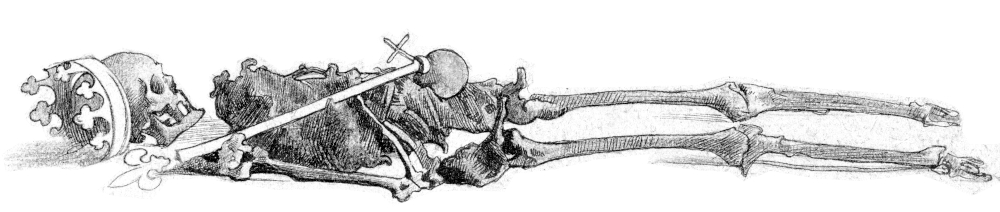
\includegraphics[keepaspectratio,width=\textwidth]{figures/skeltal-small.jpg}
\caption{\citeart{SkeletonCrown}}
\label{fig:skeltal}
\end{figure}
\lettrine{Y}{ou} may guess at the prognostics by the symptoms. What can these signs
fore tell otherwise than folly, dotage, madness, gross ignorance,
despair, obstinacy, a reprobate sense, \authorfootnote{6590}a bad end? What else can
superstition, heresy produce, but wars, tumults, uproars, torture of
souls, and despair, a desolate land, as Jeremy teacheth, cap. vii. 34.
when they commit idolatry, and walk after their own ways? how should it
be otherwise with them? what can they expect but blasting, famine,
dearth, and all the plagues of Egypt, as Amos denounceth, cap. iv.
vers. 9. 10. to be led into captivity? If our hopes be frustrate, we
sow much and bring in little, eat and have not enough, drink and are
not filled, clothe and be not warm, \&c. Haggai i. 6. we look for much
and it comes to little, whence is it? His house was waste, they came to
their own houses, vers. 9. therefore the heaven stayed his dew, the
earth his fruit. Because we are superstitious, irreligious, we do not
serve God as we ought, all these plagues and miseries come upon us;
what can we look for else but mutual wars, slaughters, fearful ends in
this life, and in the life to come eternal damnation? What is it that
hath caused so many feral battles to be fought, so much Christian blood
shed, but superstition! That Spanish inquisition, racks, wheels,
tortures, torments, whence do they proceed? from superstition. Bodine
the Frenchman, in his \authorfootnote{6591}method. hist. accounts Englishmen
barbarians, for their civil wars: but let him read those Pharsalian
fields \authorfootnote{6592}fought of late in France for their religion, their
massacres, wherein by their own relations in twenty-four years, I know
not how many millions have been consumed, whole families and cities,
and he shall find ours to be but velitations to theirs. But it hath
ever been the custom of heretics and idolaters, when they are plagued
for their sins, and God's just judgments come upon them, not to
acknowledge any fault in themselves, but still impute it unto others.
In Cyprian's time it was much controverted between him and Demetrius an
idolater, who should be the cause of those present calamities.
Demetrius laid all the fault on Christians, (and so they did ever in
the primitive church, as appears by the first book of \authorfootnote{6593}Arnobius),
\authorfootnote{6594}that there were not such ordinary showers in winter, the ripening
heat in summer, so seasonable springs, fruitful autumns, no marble
mines in the mountains, less gold and silver than of old; that
husbandmen, seamen, soldiers, all were scanted, justice, friendship,
skill in arts, all was decayed, and that through Christians' default,
and all their other miseries from them, quod dii nostri a vobis non
colantur, because they did not worship their gods. But Cyprian retorts
all upon him again, as appears by his tract against him. 'Tis true the
world is miserably tormented and shaken with wars, dearth, famine,
fire, inundations, plagues, and many feral diseases rage amongst us,
sed non ut tu quereris ista accidunt quod dii vestri a nobis non
colantur, sed quod a vobis non colatur Deus, a quibus nec quaeritur,
nec timetur, not as thou complainest, that we do not worship your Gods,
but because you are idolaters, and do not serve the true God, neither
seek him, nor fear him as you ought. Our papists object as much to us,
and account us heretics, we them; the Turks esteem of both as infidels,
and we them as a company of pagans, Jews against all; when indeed there
is a general fault in us all, and something in the very best, which may
justly deserve God's wrath, and pull these miseries upon our heads. I
will say nothing here of those vain cares, torments, needless works,
penance, pilgrimages, pseudomartyrdom, \&c. We heap upon ourselves
unnecessary troubles, observations; we punish our bodies, as in Turkey
(saith \authorfootnote{6595}Busbequius leg. Turcic. ep. 3.) one did, that was much
affected with music, and to hear boys sing, but very superstitious; an
old sibyl coming to his house, or a holy woman, (as that place yields
many) took him down for it, and told him, that in that other world he
should suffer for it; thereupon he flung his rich and costly
instruments which he had bedecked with jewels, all at once into the
fire. He was served in silver plate, and had goodly household stuff: a
little after, another religious man reprehended him in like sort, and
from thenceforth he was served in earthen vessels, last of all a decree
came forth, because Turks might not drink wine themselves, that neither
Jew nor Christian then living in Constantinople, might drink any wine
at all. In like sort amongst papists, fasting at first was generally
proposed as a good thing; after, from such meats at set times, and then
last of all so rigorously proposed, to bind the consciences upon pain
of damnation. First Friday, saith Erasmus, then Saturday, et nunc
periclitatur dies Mercurii) and Wednesday now is in danger of a fast.
\authorfootnote{6596}And for such like toys, some so miserably afflict themselves, to
despair, and death itself, rather than offend, and think themselves
good Christians in it, when as indeed they are superstitious Jews. So
saith Leonardus Fuchsius, a great physician in his time. \authorfootnote{6597}We are
tortured in Germany with these popish edicts, our bodies so taken down,
our goods so diminished, that if God had not sent Luther, a worthy man,
in time, to redress these mischiefs, we should have eaten hay with our
horses before this. \authorfootnote{6598}As in fasting, so in all other superstitious
edicts, we crucify one another without a cause, barring ourselves of
many good and lawful things, honest disports, pleasures and
recreations; for wherefore did God create them but for our use? Feasts,
mirth, music, hawking, hunting, singing, dancing, \&c. non tam
necessitatibus nostris Deus inservit, sed in delicias amamur, as Seneca
notes, God would have it so. And as Plato 2. de legibus gives out, Deos
laboriosam hominum vitam miseratos, the gods in commiseration of human
estate sent Apollo, Bacchus, and the Muses, qui cum voluptate tripudia
et soltationes nobis ducant, to be merry with mortals, to sing and
dance with us. So that he that will not rejoice and enjoy himself,
making good use of such things as are lawfully permitted, non est
temperatus, as he will, sed superstitiosus. There is nothing better for
a man, than that he should eat and drink, and that he should make his
soul enjoy good in his labour, Eccles. ii. 24. And as \authorfootnote{6599}one said of
hawking and hunting, tot solatia in hac aegri orbis calamitate,
mortalibus taediis deus objecit, I say of all honest recreations, God
hath therefore indulged them to refresh, ease, solace and comfort us.
But we are some of us too stern, too rigid, too precise, too grossly
superstitious, and whilst we make a conscience of every toy, with touch
not, taste not, \&c., as those Pythagoreans of old, and some Indians
now, that will eat no flesh, or suffer any living creature to be
killed, the Bannians about Guzzerat; we tyrannise over our brother's
soul, lose the right use of many good gifts; honest \authorfootnote{6600}sports, games
and pleasant recreations, \authorfootnote{6601}punish ourselves without a cause, lose
our liberties, and sometimes our lives. Anno 1270, at \authorfootnote{6602}Magdeburg
in Germany, a Jew fell into a privy upon a Saturday, and without help
could not possibly get out; he called to his fellows for succour, but
they denied it, because it was their Sabbath, non licebat opus manuum
exercere; the bishop hearing of it, the next day forbade him to be
pulled out, because it was our Sunday. In the mean time the wretch died
before Monday. We have myriads of examples in this kind amongst those
rigid Sabbatarians, and therefore not without good cause,
\authorfootnote{6603}Intolerabilem pertubationem Seneca calls it, as well he might, an
intolerable perturbation, that causeth such dire events, folly,
madness, sickness, despair, death of body and soul, and hell itself.

%SUBSECT. V.-_Cure of Religious Melancholy_.
\section{Cure of Religious Melancholy.}

\lettrine{T}{o} purge the world of idolatry and superstition, will require some
monster-taming Hercules, a divine Aesculapius, or Christ himself to
come in his own person, to reign a thousand years on earth before the
end, as the Millenaries will have him. They are generally so
refractory, self-conceited, obstinate, so firmly addicted to that
religion in which they have been bred and brought up, that no
persuasion, no terror, no persecution, can divert them. The
consideration of which, hath induced many commonwealths to suffer them
to enjoy their consciences as they will themselves: a toleration of
Jews is in most provinces of Europe. In Asia they have their
synagogues: Spaniards permit Moors to live amongst them: the
Mogullians, Gentiles: the Turks all religions. In Europe, Poland and
Amsterdam are the common sanctuaries. Some are of opinion, that no man
ought to be compelled for conscience' sake, but let him be of what
religion he will, he may be saved, as Cornelius was formerly accepted,
Jew, Turks, Anabaptists, \&c. If he be an honest man, live soberly, and
civilly in his profession, (Volkelius, Crellius, and the rest of the
Socinians, that now nestle themselves about Krakow and Rakow in Poland,
have renewed this opinion) serve his own God, with that fear and
reverence as he ought. Sua cuique civitati (Laeli) religio sit, nostra
nobis, Tully thought fit every city should be free in this behalf,
adore their own Custodes et Topicos Deos, tutelar and local gods, as
Symmachus calls them. Isocrates adviseth Demonicus, when he came to a
strange city, to \authorfootnote{6604}worship by all means the gods of the place, et
unumquemque, Topicum deum sic coli oportere, quomodo ipse praeceperit:
which Cecilius in \authorfootnote{6605}Minutius labours, and would have every nation
sacrorum ritus gentiles habere et deos colere municipes, keep their own
ceremonies, worship their peculiar gods, which Pomponius Mela reports
of the Africans, Deos suos patrio more venerantur, they worship their
own gods according to their own ordination. For why should any one
nation, as he there pleads, challenge that universality of God, Deum
suum quem nec ostendunt, nec vident, discurrantem silicet et ubique
praesentem, in omnium mores, actus, et occultas, cogitationes
inquirentem, \&c., as Christians do: let every province enjoy their
liberty in this behalf, worship one God, or all as they will, and are
informed. The Romans built altars Diis Asiae, Europae, Lybiae, diis
ignotis et peregrinis: others otherwise, \&c. Plinius Secundus, as
appears by his Epistle to Trajan, would not have the Christians so
persecuted, and in some time of the reign of Maximinus, as we find it
registered in Eusebius lib. 9. cap. 9. there was a decree made to this
purpose, Nullus cogatur invitus ad hunc vel illum deorum cultum, let no
one be compelled against his will to worship any particular deity, and
by Constantine in the 19th year of his reign as \authorfootnote{6606}Baronius
informeth us, Nemo alteri exhibeat molestiam, quod cujusque animus
vult, hoc quisque transigat, new gods, new lawgivers, new priests, will
have new ceremonies, customs and religions, to which every wise man as
a good formalist should accommodate himself.
\authorfootnote{6607}Saturnus periit, perierunt et sua jura,
Sub Jove nunc mundus, jussa sequare Jovis.

The said Constantine the emperor, as Eusebius writes, flung down and
demolished all the heathen gods, silver, gold statues, altars, images
and temples, and turned them all to Christian churches, infestus
gentilium monumentis ludibrio exposuit; the Turk now converts them
again to Mahometan mosques. The like edict came forth in the reign of
Arcadius and Honorius. \authorfootnote{6608}Symmachus the orator in his days, to
procure a general toleration, used this argument, \authorfootnote{6609}Because God is
immense and infinite, and his nature cannot perfectly be known, it is
convenient he should be as diversely worshipped, as every man shall
perceive or understand. It was impossible, he thought, for one religion
to be universal: you see that one small province can hardly be ruled by
one law, civil or spiritual; and how shall so many distinct and vast
empires of the world be united into one? It never was, never will be
Besides, if there be infinite planetary and firmamental worlds, as
\authorfootnote{6610}some will, there be infinite genii or commanding spirits
belonging to each of them; and so, per consequens (for they will be all
adored), infinite religions. And therefore let every territory keep
their proper rites and ceremonies, as their dii tutelares will, so
Tyrius calls them, and according to the quarter they hold, their own
institutions, revelations, orders, oracles, which they dictate from
time to time, or teach their own priests or ministers. This tenet was
stiffly maintained in Turkey not long since, as you may read in the
third epistle of Busbequius, \authorfootnote{6611}that all those should participate of
eternal happiness, that lived a holy and innocent life, what religion
soever they professed. Rustan Bassa was a great patron of it; though
Mahomet himself was sent virtute gladdi, to enforce all, as he writes
in his Alcoran, to follow him. Some again will approve of this for
Jews, Gentiles, infidels, that are out of the fold, they can be content
to give them all respect and favour, but by no means to such as are
within the precincts of our own church, and called Christians, to no
heretics, schismatics, or the like; let the Spanish inquisition, that
fourth fury, speak of some of them, the civil wars and massacres in
France, our Marian times. \authorfootnote{6612}Magillianus the Jesuit will not admit
of conference with a heretic, but severity and rigour to be used, non
illis verba reddere, sed furcas, figere oportet; and Theodosius is
commended in Nicephorus, lib. 12. cap. 15. \authorfootnote{6613}That he put all
heretics to silence. Bernard. Epist. 180, will have club law, fire and
sword for heretics, \authorfootnote{6614}compel them, stop their mouths not with
disputations, or refute them with reasons, but with fists; and this is
their ordinary practice. Another company are as mild on the other side;
to avoid all heart-burning, and contentious wars and uproars, they
would have a general toleration in every kingdom, no mulct at all, no
man for religion or conscience be put to death, which \authorfootnote{6615}Thuanus the
French historian much favours; our late Socinians defend; Vaticanus
against Calvin in a large Treatise in behalf of Servetus, vindicates;
Castilio, \&c., Martin Ballius and his companions, maintained this
opinion not long since in France, whose error is confuted by Beza in a
just volume. The medium is best, and that which Paul prescribes, Gal.
i. If any man shall fall by occasion, to restore such a one with the
spirit of meekness, by all fair means, gentle admonitions; but if that
will not take place, Post unam et alteram admonitionem haereticum
devita, he must be excommunicate, as Paul did by Hymenaeus, delivered
over to Satan. Immedicabile vulnus ense recidendum est. As Hippocrates
said in physic, I may well say in divinity, Quae ferro non curantur,
ignis curat. For the vulgar, restrain them by laws, mulcts, burn their
books, forbid their conventicles; for when the cause is taken away, the
effect will soon cease. Now for prophets, dreamers, and such rude silly
fellows, that through fasting, too much meditation, preciseness, or by
melancholy, are distempered: the best means to reduce them ad sanam
mentem, is to alter their course of life, and with conference, threats,
promises, persuasions, to intermix physic. Hercules de Saxonia, had
such a prophet committed to his charge in Venice, that thought he was
Elias, and would fast as he did; he dressed a fellow in angel's attire,
that said he came from heaven to bring him divine food, and by that
means stayed his fast, administered his physic; so by the meditation of
this forged angel he was cured. \authorfootnote{6616}Rhasis an Arabian, cont. lib. 1.
cap. 9, speaks of a fellow that in like case complained to him, and
desired his help: I asked him (saith he) what the matter was; he
replied, I am continually meditating of heaven and hell, and methinks I
see and talk with fiery spirits, and smell brimstone, \&c., and am so
carried away with these conceits, that I can neither eat, nor sleep,
nor go about my business: I cured him (saith Rhasis) partly by
persuasion, partly by physic, and so have I done by many others. We
have frequently such prophets and dreamers amongst us, whom we
persecute with fire and faggot: I think the most compendious cure, for
some of them at least, had been in Bedlam. Sed de his satis.

%MEMB. II.

%SUBSECT. I.-_Religious Melancholy in defect; parties affected, Epicures, Atheists, Hypocrites, worldly secure, Carnalists; all impious persons, impenitent sinners, \&c._
\section[Religious Melancholy in defect]{Religious Melancholy in defect; parties affected, Epicures, Atheists, Hypocrites, worldly secure, Carnalists; all impious persons, impenitent sinners, \&c.}

\lettrine{I}{n} that other extreme or defect of this love of God, knowledge, faith,
fear, hope, \&c. are such as err both in doctrine and manners,
Sadducees, Herodians, libertines, politicians: all manner of atheists,
epicures, infidels, that are secure, in a reprobate sense, fear not God
at all, and such are too distrustful and timorous, as desperate persons
be. That grand sin of atheism or impiety, \authorfootnote{6617}Melancthon calls it
monstrosam melancholiam, monstrous melancholy; or venenatam
melancholiam, poisoned melancholy. A company of Cyclops or giants, that
war with the gods, as the poets feigned, antipodes to Christians, that
scoff at all religion, at God himself, deny him and all his attributes,
his wisdom, power, providence, his mercy and judgment.
\authorfootnote{6618}Esse aliquos manes, et subterranea regna,
Et contum, et Stygio ranas in gurgite nigras,
Atque una transire vadum tot millia cymba,
Nec pueri credunt, nisi qui nondum aere lavantur.

That there is either heaven or hell, resurrection of the dead, pain,
happiness, or world to come, credat Judaeus Apella; for their parts
they esteem them as so many poet's tales, bugbears, Lucian's Alexander;
Moses, Mahomet, and Christ are all as one in their creed. When those
bloody wars in France for matters of religion (saith \authorfootnote{6619}Richard
Dinoth) were so violently pursued between Huguenots and Papists, there
was a company of good fellows laughed them all to scorn, for being such
superstitious fools, to lose their wives and fortunes, accounting
faith, religion, immortality of the soul, mere fopperies and illusions.
Such loose \authorfootnote{6620}atheistical spirits are too predominant in all
kingdoms. Let them contend, pray, tremble, trouble themselves that
will, for their parts, they fear neither God nor devil; but with that
Cyclops in Euripides,
Haud ulla numina expavescunt caelitum,
Sed victimas uni deorum maximo,
Ventri offerunt, deos ignorant caeteros.

They fear no God but one,
They sacrifice to none.
But belly, and him adore,
For gods they know no more.

Their God is their belly, as Paul saith, Sancta mater saturitas;-quibus
in solo vivendi causa palato est. The idol, which they worship and
adore, is their mistress; with him in Plautus, mallem haec mulier me
amet quam dii, they had rather have her favour than the gods'. Satan is
their guide, the flesh is their instructor, hypocrisy their counsellor,
vanity their fellow-soldier, their will their law, ambition their
captain, custom their rule; temerity, boldness, impudence their art,
toys their trading, damnation their end. All their endeavours are to
satisfy their lust and appetite, how to please their genius, and to be
merry for the present, Ede, lude, bibe, post mortem nulla
voluptas.\authorfootnote{6621}The same condition is of men and of beasts; as the one
dieth, so dieth the other, Eccles. iii. 19. The world goes round,
\authorfootnote{6622}---truditur dies die,
Novaeque pergunt interire Lunae:

\authorfootnote{6623}They did eat and drink of old, marry, bury, bought, sold,
planted, built, and will do still. \authorfootnote{6624}Our life is short and tedious,
and in the death of a man there is no recovery, neither was any man
known that hath returned from the grave; for we are born at all
adventure, and we shall be hereafter as though we had never been; for
the breath is as smoke in our nostrils, \&c., and the spirit vanisheth
as the soft air. \authorfootnote{6625}Come let us enjoy the pleasures that are
present, let us cheerfully use the creatures as in youth, let us fill
ourselves with costly wine and ointments, let not the flower of our
life pass by us, let us crown ourselves with rose-buds before they are
withered, \&c. \authorfootnote{6626}Vivamus mea Lesbia et amemus, \&c. \authorfootnote{6627} Come let
us take our fill of love, and pleasure in dalliance, for this is our
portion, this is our lot.
Tempora labuntur, tacitisque senescimus annis.\authorfootnote{6628} For the rest of
heaven and hell, let children and superstitious fools believe it: for
their parts, they are so far from trembling at the dreadful day of
judgment that they wish with Nero, Me vivo fiat, let it come in their
times: so secure, so desperate, so immoderate in lust and pleasure, so
prone to revenge that, as Paterculus said of some caitiffs in his time
in Rome, Quod nequiter ausi, fortiter executi: it shall not be so
wickedly attempted, but as desperately performed, whatever they take in
hand. Were it not for God's restraining grace, fear and shame, temporal
punishment, and their own infamy, they would. Lycaon-like exenterate,
as so many cannibals eat up, or Cadmus' soldiers consume one another.
These are most impious, and commonly professed atheists, that never use
the name of God but to swear by it; that express nought else but
epicurism in their carriage, or hypocrisy; with Pentheus they neglect
and contemn these rites and religious ceremonies of the gods; they will
be gods themselves, or at least socii deorum. Divisum imperium cum Jove
Caesar habet. Caesar divides the empire with Jove. Aproyis, an Egyptian
tyrant, grew, saith \authorfootnote{6629}Herodotus, to that height of pride, insolency
of impiety, to that contempt of Gods and men, that he held his kingdom
so sure, ut a nemine deorum aut hominum sibi eripi posset, neither God
nor men could take it from him. \authorfootnote{6630}A certain blasphemous king of
Spain (as \authorfootnote{6631}Lansius reports) made an edict, that no subject of his,
for ten years' space, should believe in, call on, or worship any god.
And as \authorfootnote{6632}Jovius relates of Mahomet the Second, that sacked
Constantinople, he so behaved himself, that he believed neither Christ
nor Mahomet; and thence it came to pass, that he kept his word and
promise no farther than for his advantage, neither did he care to
commit any offence to satisfy his lust. I could say the like of many
princes, many private men (our stories are full of them) in times past,
this present age, that love, fear, obey, and perform all civil duties
as they shall find them expedient or behoveful to their own ends.
Securi adversus Deos, securi adversus homines, votis non est opus,
which \authorfootnote{6633} Tacitus reports of some Germans, they need not pray, fear,
hope, for they are secure, to their thinking, both from Gods and men.
Bulco Opiliensis, sometime Duke of \authorfootnote{6634}Silesia, was such a one to a
hair; he lived (saith \authorfootnote{6635}Aeneas Sylvius) at \authorfootnote{6636}Vratislavia, and
was so mad to satisfy his lust, that he believed neither heaven nor
hell, or that the soul was immortal, but married wives, and turned them
up as he thought fit, did murder and mischief, and what he list
himself. This duke hath too many followers in our days: say what you
can, dehort, exhort, persuade to the contrary, they are no more
moved,-quam si dura, silex aut stet Marpesia cautes, than so many
stocks, and stones; tell them of heaven and hell, 'tis to no purpose,
laterem lavas, they answer as Ataliba that Indian prince did friar
Vincent, \authorfootnote{6637}when he brought him a book, and told him all the
mysteries of salvation, heaven and hell, were contained in it: he
looked upon it, and said he saw no such matter, asking withal, how he
knew it: they will but scoff at it, or wholly reject it. Petronius in
Tacitus, when he was now by Nero's command bleeding to death, audiebat
amicos nihil referentes de immortalitate animae, aut sapientum
placitis, sed levia carmina et faciles versus; instead of good counsel
and divine meditations, he made his friends sing him bawdy verses and
scurrilous songs. Let them take heaven, paradise, and that future
happiness that will, bonum est esse hic, it is good being here: there
is no talking to such, no hope of their conversion, they are in a
reprobate sense, mere carnalists, fleshly minded men, which howsoever
they may be applauded in this life by some few parasites, and held for
worldly wise men. \authorfootnote{6638}They seem to me (saith Melancthon) to be as mad
as Hercules was when he raved and killed his wife and children. A
milder sort of these atheistical spirits there are that profess
religion, but timide et haesitanter, tempted thereunto out of that
horrible consideration of diversity of religions, which are and have
been in the world (which argument Campanella, Atheismi Triumphati, cap.
9. both urgeth and answers), besides the covetousness, imposture, and
knavery of priests, quae faciunt (as \authorfootnote{6639}Postellus observes) ut rebus
sacris minus faciant fidem; and those religions some of them so
fantastical, exorbitant, so violently maintained with equal constancy
and assurance; whence they infer, that if there be so many religious
sects, and denied by the rest, why may they not be all false? or why
should this or that be preferred before the rest? The sceptics urge
this, and amongst others it is the conclusion of Sextus Empericus, lib.
3. advers. Mathematicos: after many philosophical arguments and reasons
pro and con that there are gods, and again that there are no gods, he
so concludes, cum tot inter se pugnent, \&c. Una tantum potest esse
vera, as Tully likewise disputes: Christians say, they alone worship
the true God, pity all other sects, lament their case; and yet those
old Greeks and Romans that worshipped the devil, as the Chinese now do,
aut deos topicos, their own gods; as Julian the apostate,
\authorfootnote{6640}Cecilius in Minutius, Celsus and Porphyrius the philosopher
object: and as Machiavel contends, were much more noble, generous,
victorious, had a more flourishing commonwealth, better cities, better
soldiers, better scholars, better wits. Their gods overcame our gods,
did as many miracles, \&c. Saint Cyril, Arnobius, Minutius, with many
other ancients of late, Lessius, Morneus, Grotius de Verit. Relig.
Christianae, Savanarola de Verit. Fidei Christianae, well defend; but
Zanchius, \authorfootnote{6641}Campanella, Marinus Marcennus, Bozius, and Gentillettus
answer all these atheistical arguments at large. But this again
troubles many as of old, wicked men generally thrive, professed
atheists thrive,
\authorfootnote{6642}Nullos esse Deos, inane coelum,
Affirmat Selius: probatque, quod se
Factum, dum negat haec, videt beatum.

There are no gods, heavens are toys,
Selius in public justifies;
Because that whilst he thus denies
Their deities, he better thrives.

This is a prime argument: and most part your most sincere, upright,
honest, and \authorfootnote{6643}good men are depressed, The race is not to the swift,
nor the battle to the strong (Eccles. ix. 11.), nor yet bread to the
wise, favour nor riches to men of understanding, but time and chance
comes to all. There was a great plague in Athens (as Thucydides, lib.
2. relates), in which at last every man, with great licentiousness, did
what he list, not caring at all for God's or men's laws. Neither the
fear of God nor laws of men (saith he) awed any man, because the plague
swept all away alike, good and bad; they thence concluded it was alike
to worship or not worship the gods, since they perished all alike. Some
cavil and make doubts of scripture itself: it cannot stand with God's
mercy, that so many should be damned, so many bad, so few good, such
have and hold about religions, all stiff on their side, factious alike,
thrive alike, and yet bitterly persecuting and damning each other; It
cannot stand with God's goodness, protection, and providence (as
\authorfootnote{6644}Saint Chrysostom in the Dialect of such discontented persons) to
see and suffer one man to be lame, another mad, a third poor and
miserable all the days of his life, a fourth grievously tormented with
sickness and aches, to his last hour. Are these signs and works of
God's providence, to let one man be deaf, another dumb? A poor honest
fellow lives in disgrace, woe and want, wretched he is; when as a
wicked caitiff abounds in superfluity of wealth, keeps whores,
parasites, and what he will himself: Audis Jupiter haec? Talia multa
connectentes, longum reprehensionis sermonem erga Dei providentiam
contexunt. \authorfootnote{6645}Thus they mutter and object (see the rest of their
arguments in Marcennus in Genesin, and in Campanella, amply confuted),
with many such vain cavils, well known, not worthy the recapitulation
or answering: whatsoever they pretend, they are interim of little or no
religion.
Cousin-germans to these men are many of our great philosophers and
deists, who, though they be more temperate in this life, give many good
moral precepts, honest, upright, and sober in their conversation, yet
in effect they are the same (accounting no man a good scholar that is
not an atheist), nimis altum sapiunt, too much learning makes them mad.
Whilst they attribute all to natural causes, \authorfootnote{6646}contingence of all
things, as Melancthon calls them, Pertinax hominum genus, a peevish
generation of men, that misled by philosophy, and the devil's
suggestion, their own innate blindness, deny God as much as the rest,
hold all religion a fiction, opposite to reason and philosophy, though
for fear of magistrates, saith \authorfootnote{6647}Vaninus, they durst not publicly
profess it. Ask one of them of what religion he is, he scoffingly
replies, a philosopher, a Galenist, an \authorfootnote{6648}Averroist, and with
Rabelais a physician, a peripatetic, an epicure. In spiritual things
God must demonstrate all to sense, leave a pawn with them, or else seek
some other creditor. They will acknowledge Nature and Fortune, yet not
God: though in effect they grant both: for as Scaliger defines, Nature
signifies God's ordinary power; or, as Calvin writes, Nature is God's
order, and so things extraordinary may be called unnatural: Fortune his
unrevealed will; and so we call things changeable that are beside
reason and expectation. To this purpose \authorfootnote{6649}Minutius in Octavio, and
\authorfootnote{6650} Seneca well discourseth with them, lib. 4. de beneficiis, cap.
5, 6, 7. They do not understand what they say; what is Nature but God?
call him what thou wilt, Nature, Jupiter, he hath as many names as
offices: it comes all to one pass, God is the fountain of all, the
first Giver and Preserver, from whom all things depend, \authorfootnote{6651}a quo, et
per quem omnia, Nam quocunque vides Deus est, quocunque moveris, God is
all in all, God is everywhere, in every place. And yet this Seneca,
that could confute and blame them, is all out as much to be blamed and
confuted himself, as mad himself; for he holds fatum Stoicum, that
inevitable Necessity in the other extreme, as those Chaldean
astrologers of old did, against whom the prophet Jeremiah so often
thunders, and those heathen mathematicians, Nigidius Figulus,
magicians, and Priscilianists, whom St. Austin so eagerly confutes,
those Arabian questionaries, Novem Judices, Albumazer, Dorotheus, \&c.,
and our countryman \authorfootnote{6652}Estuidus, that take upon them to define out of
those great conjunction of stars, with Ptolomeus, the periods of
kingdoms, or religions, of all future accidents, wars, plagues,
schisms, heresies, and what not? all from stars, and such things, saith
Maginus, Quae sibi et intelligentiis suis reservavit Deus, which God
hath reserved to himself and his angels, they will take upon them to
foretell, as if stars were immediate, inevitable causes of all future
accidents. Caesar Vaninus, in his book de admirandis naturae Arcanis,
dial. 52. de oraculis, is more free, copious, and open, in this
explication of this astrological tenet of Ptolemy, than any of our
modern writers, Cardan excepted, a true disciple of his master
Pomponatius; according to the doctrine of Peripatetics, he refers all
apparitions, prodigies, miracles, oracles, accidents, alterations of
religions, kingdoms, \&c. (for which he is soundly lashed by Marinus
Mercennus, as well he deserves), to natural causes (for spirits he will
not acknowledge), to that light, motion, influences of heavens and
stars, and to the intelligences that move the orbs. Intelligentia quae,
movet orbem mediante coelo, \&c. Intelligences do all: and after a long
discourse of miracles done of old, si haec daemones possint, cur non et
intelligentiae, coelorum motrices? And as these great conjunctions,
aspects of planets, begin or end, vary, are vertical and predominant,
so have religions, rites, ceremonies, and kingdoms their beginning,
progress, periods, in urbibus, regibus, religionibus, ac in
particularibus hominibus, haec vera ac manifesta, sunt, ut Aristoteles
innuere videtur, et quotidiana docet experientia, ut historias
perlegens videbit; quid olim in Gentili lege Jove sanctius et
illustrius? quid nunc vile magis et execrandum? Ita coelestia corpora
pro mortalium beneficio religiones aedificant, et cum cessat influxus,
cessat lex,\authorfootnote{6653} \&c. And because, according to their tenets, the world
is eternal, intelligences eternal, influences of stars eternal,
kingdoms, religions, alterations shall be likewise eternal, and run
round after many ages; Atque iterum ad Troiam magnus mittetur Achilles;
renascentur religiones, et ceremoniae, res humanae in idem recident,
nihil nunc quod non olim fuit, et post saeculorum revolutiones alias
est, erit,\authorfootnote{6654}\&c. idem specie, saith Vaninus, non individuo quod
Plato significavit. These (saith mine \authorfootnote{6655}author), these are the
decrees of Peripatetics, which though I recite, in obsequium
Christianae fidei detestor, as I am a Christian I detest and hate. Thus
Peripatetics and astrologians held in former times, and to this effect
of old in Rome, saith Dionysius Halicarnassus, lib. 7, when those
meteors and prodigies appeared in the air, after the banishment of
Coriolanus, \authorfootnote{6656} Men were diversely affected: some said they were
God's just judgments for the execution of that good man, some referred
all to natural causes, some to stars, some thought they came by chance,
some by necessity decreed ab initio, and could not be altered. The two
last opinions of necessity and chance were, it seems, of greater note
than the rest.
\authorfootnote{6657}Sunt qui in Fortunae jam casibus omnia ponunt,
Et mundum credunt nullo rectore moveri,
Natura, volvente vices, \&c.

For the first of chance, as \authorfootnote{6658}Sallust likewise informeth us, those
old Romans generally received; They supposed fortune alone gave
kingdoms and empires, wealth, honours, offices: and that for two
causes; first, because every wicked base unworthy wretch was preferred,
rich, potent, \&c.; secondly, because of their uncertainty, though never
so good, scarce any one enjoyed them long: but after, they began upon
better advice to think otherwise, that every man made his own fortune.
The last of Necessity was Seneca's tenet, that God was alligatus causis
secundis, so tied to second causes, to that inexorable Necessity, that
he could alter nothing of that which was once decreed; sic erat in
fatis, it cannot be altered, semel jussit, semper paret Deus, nulla vis
rumpit, nullae preces, nec ipsum fulmen, God hath once said it, and it
must for ever stand good, no prayers, no threats, nor power, nor
thunder itself can alter it. Zeno, Chrysippus, and those other Stoics,
as you may read in Tully 2. de divinatione, Gellius, lib. 6. cap. 2.
\&c., maintained as much. In all ages, there have been such, that either
deny God in all, or in part; some deride him, they could have made a
better world, and ruled it more orderly themselves, blaspheme him,
derogate at their pleasure from him. 'Twas so in \authorfootnote{6659}Plato's time,
Some say there be no gods, others that they care not for men, a middle
sort grant both. Si non sit Deus, unde mala? si sit Deus, unde mala? So
Cotta argues in Tully, why made he not all good, or at least tenders
not the welfare of such as are good? As the woman told Alexander, if he
be not at leisure to hear causes, and redress them, why doth he reign?
\authorfootnote{6660}Sextus Empericus hath many such arguments. Thus perverse men
cavil. So it will ever be, some of all sorts, good, bad, indifferent,
true, false, zealous, ambidexters, neutralists, lukewarm, libertines,
atheists, \&c. They will see these religious sectaries agree amongst
themselves, be reconciled all, before they will participate with, or
believe any: they think in the meantime (which \authorfootnote{6661}Celsus objects,
and whom Origen confutes), We Christians adore a person put to
\authorfootnote{6662}death with no more reason than the barbarous Getes worshipped
Zamolxis, the Cilicians Mopsus, the Thebans Amphiaraus, and the
Lebadians Trophonius; one religion is as true as another, new fangled
devices, all for human respects; great-witted Aristotle's works are as
much authentical to them as Scriptures, subtle Seneca's Epistles as
canonical as St. Paul's, Pindarus' Odes as good as the Prophet David's
Psalms, Epictetus' Enchiridion equivalent to wise Solomon's Proverbs.
They do openly and boldly speak this and more, some of them, in all
places and companies. \authorfootnote{6663}Claudius the emperor was angry with Heaven,
because it thundered, and challenged Jupiter into the field; with what
madness! saith Seneca; he thought Jupiter could not hurt him, but he
could hurt Jupiter. Diagoras, Demonax, Epicurus, Pliny, Lucian,
Lucretius,-Contemptorque Deum Mezentius, professed atheists all in
their times: though not simple atheists neither, as Cicogna proves,
lib. 1. cap. 1. they scoffed only at those Pagan gods, their plurality,
base and fictitious offices. Gilbertus Cognatus labours much, and so
doth Erasmus, to vindicate Lucian from scandal, and there be those that
apologise for Epicurus, but all in vain; Lucian scoffs at all, Epicurus
he denies all, and Lucretius his scholar defends him in it:
\authorfootnote{6664}Humana ante oculua foede cum vita jaceret
In terris oppressa gravi cum religione,
Quae caput a coeli regionibus ostendebat,
Horribili super aspectu mortalibus instans, \&c.

When human kind was drench'd in superstition,
With ghastly looks aloft, which frighted mortal men, \&c.

He alone, like another Hercules, did vindicate the world from that
monster. Uncle \authorfootnote{6665}Pliny, lib. 2. cap. 7. nat. hist. and lib. 7. cap.
55, in express words denies the immortality of the soul. \authorfootnote{6666}Seneca
doth little less, lib. 7. epist. 55. ad Lucilium, et lib. de consol. ad
Martiam, or rather more. Some Greek Commentators would put as much upon
Job, that he should deny resurrection, \&c., whom Pineda copiously
confutes in cap. 7. Job, vers. 9. Aristotle is hardly censured of some,
both divines and philosophers. St. Justin in Peraenetica ad Gentes,
Greg. Nazianzen. in disput. adversus Eun., Theodoret, lib. 5. de curat.
graec. affec., Origen. lib. de principiis. Pomponatius justifies in his
Tract (so styled at least) De immortalitate Animae, Scaliger (who would
forswear himself at any time, saith Patritius, in defence of his great
master Aristotle), and Dandinus, lib. 3. de anima, acknowledge as much.
Averroes oppugns all spirits and supreme powers; of late Brunus
(infelix Brunus, \authorfootnote{6667}Kepler calls him), Machiavel, Caesar Vaninus
lately burned at Toulouse in France, and Pet. Aretine, have publicly
maintained such atheistical paradoxes, \authorfootnote{6668}with that Italian
Boccaccio with his fable of three rings, \&c., ex quo infert haud posse
internosci, quae sit verior religio, Judaica, Mahometana, an
Christiana, quoniam eadem signa, \&c., from which he infers, that it
cannot be distinguished which is the true religion, Judaism,
Mahommedanism, or Christianity, \&c. \authorfootnote{6669}Marinus Mercennus suspects
Cardan for his subtleties, Campanella, and Charron's Book of Wisdom,
with some other Tracts, to savour of \authorfootnote{6670}atheism: but amongst the
rest that pestilent book de tribus mundi impostoribus, quem sine
horrore (inquit) non legas, et mundi Cymbalum dialogis quatuor
contentum, anno 1538, auctore Peresio, Parisiis excusum, \authorfootnote{6671}\&c. And
as there have been in all ages such blasphemous spirits, so there have
not been wanting their patrons, protectors, disciples and adherents.
Never so many atheists in Italy and Germany, saith \authorfootnote{6672}Colerus, as in
this age: the like complaint Mercennus makes in France, 50,000 in that
one city of Paris. Frederic the Emperor, as \authorfootnote{6673}Matthew Paris records
licet non sit recitabile (I use his own words) is reported to have
said, Tres praestigiatores, Moses, Christus, et Mahomet, uti mundo
dominarentur, totum populum sibi contemporaneum se duxisse. (Henry, the
Landgrave of Hesse, heard him speak it,) Si principes imperii
institutioni meae adhaererent, ego multo meliorem modum credendi et
vivendi ordinarem.
To these professed atheists, we may well add that impious and carnal
crew of worldly-minded men, impenitent sinners, that go to hell in a
lethargy, or in a dream; who though they be professed Christians, yet
they will nulla pallescere culpa, make a conscience of nothing they do,
they have cauterised consciences, and are indeed in a reprobate sense,
past all feeling, have given themselves over to wantonness, to work all
manner of uncleanness even with greediness, Ephes. iv. 19. They do know
there is a God, a day of judgment to come, and yet for all that, as
Hugo saith, ita comedunt ac dormiunt, ac si diem judicii evasissent;
ita ludunt ac rident, ac si in coelis cum Deo regnarent: they are as
merry for all the sorrow, as if they had escaped all dangers, and were
in heaven already:
\authorfootnote{6674}---Metus omnes, et inexorabile fatum
Subjecit pedibus, strepitumque Acherontis avari.

Those rude idiots and ignorant persons, that neglect and contemn the
means of their salvation, may march on with these; but above all
others, those Herodian temporizing statesmen, political Machiavellians
and hypocrites, that make a show of religion, but in their hearts laugh
at it. Simulata sanctitas duplex iniquitas; they are in a double fault,
that fashion themselves to this world, which \authorfootnote{6675}Paul forbids, and
like Mercury, the planet, are good with good, bad with bad. When they
are at Rome, they do there as they see done, puritans with puritans,
papists with papists; omnium horarum homines, formalists, ambidexters,
lukewarm Laodiceans. \authorfootnote{6676}All their study is to please, and their god
is their commodity, their labour to satisfy their lusts, and their
endeavours to their own ends. Whatsoever they pretend, or in public
seem to do, \authorfootnote{6677}With the fool in their hearts, they say there is no
God. Heus tu-de Jove quid sentis? Hulloa! what is your opinion about a
Jupiter? Their words are as soft as oil, but bitterness is in their
hearts; like \authorfootnote{6678}Alexander VI. so cunning dissemblers, that what they
think they never speak. Many of them are so close, you can hardly
discern it, or take any just exceptions at them; they are not factious,
oppressors as most are, no bribers, no simoniacal contractors, no such
ambitious, lascivious persons as some others are, no drunkards, sobrii
solem vident orientem, sobrii vident occidentem, they rise sober, and
go sober to bed, plain dealing, upright, honest men, they do wrong to
no man, and are so reputed in the world's esteem at least, very zealous
in religion, very charitable, meek, humble, peace-makers, keep all
duties, very devout, honest, well spoken of, beloved of all men: but he
that knows better how to judge, he that examines the heart, saith they
are hypocrites, Cor dolo plenum; sonant vitium percussa maligne, they
are not sound within. As it is with writers \authorfootnote{6679}oftentimes, Plus
sanctimoniae, in libello, quam libelli auctore, more holiness is in the
book than in the author of it: so 'tis with them: many come to church
with great Bibles, whom Cardan said he could not choose but laugh at,
and will now and then dare operam Augustino, read Austin, frequent
sermons, and yet professed usurers, mere gripes, tota vitae ratio
epicurea est; all their life is epicurism and atheism, come to church
all day, and lie with a courtesan at night. Qui curios simulant et
Bacchanalia vivunt, they have Esau's hands, and Jacob's voice: yea, and
many of those holy friars, sanctified men, Cappam, saith Hierom, et
cilicium induunt, sed intus latronem tegunt. They are wolves in sheep's
clothing, Introrsum turpes, speciosi pelle decora, Fair without, and
most foul within. \authorfootnote{6680}Latet plerumque sub tristi amictu lascivia, et
deformis horror vili veste tegitur; ofttimes under a mourning weed lies
lust itself, and horrible vices under a poor coat. But who can examine
all those kinds of hypocrites, or dive into their hearts? ]f we may
guess at the tree by the fruit, never so many as in these days; show me
a plain-dealing true honest man: Et pudor, et probitas, et timor omnis
abest. He that shall but look into their lives, and see such enormous
vices, men so immoderate in lust, unspeakable in malice, furious in
their rage, flattering and dissembling (all for their own ends) will
surely think they are not truly religious, but of an obdurate heart,
most part in a reprobate sense, as in this age. But let them carry it
as they will for the present, dissemble as they can, a time will come
when they shall be called to an account, their melancholy is at hand,
they pull a plague and curse upon their own heads, thesaurisant iram
Dei. Besides all such as are in deos contumeliosi, blaspheme, contemn,
neglect God, or scoff at him, as the poets feign of Salmoneus, that
would in derision imitate Jupiter's thunder, he was precipitated for
his pains, Jupiter intonuit contra, \&c. so shall they certainly rue it
in the end, (\authorfootnote{6681}in se spuit, qui in coelum spuit), their doom's at
hand, and hell is ready to receive them.
Some are of opinion, that it is in vain to dispute with such
atheistical spirits in the meantime, 'tis not the best way to reclaim
them. Atheism, idolatry, heresy, hypocrisy, though they have one common
root, that is indulgence to corrupt affection, yet their growth is
different, they have divers symptoms, occasions, and must have several
cures and remedies. 'Tis true some deny there is any God, some confess,
yet believe it not; a third sort confess and believe, but will not live
after his laws, worship and obey him: others allow God and gods
subordinate, but not one God, no such general God, non talem deum, but
several topic gods for several places, and those not to persecute one
another for any difference, as Socinus will, but rather love and
cherish.
To describe them in particular, to produce their arguments and reasons,
would require a just volume, I refer them therefore that expect a more
ample satisfaction, to those subtle and elaborate treatises, devout and
famous tracts of our learned divines (schoolmen amongst the rest, and
casuists) that have abundance of reasons to prove there is a God, the
immortality of the soul, \&c., out of the strength of wit and philosophy
bring irrefragable arguments to such as are ingenuous and well
disposed; at the least, answer all cavils and objections to confute
their folly and madness, and to reduce them, si fieri posset, ad sanam
mentem, to a better mind, though to small purpose many times. Amongst
others consult with Julius Caesar Lagalla, professor of philosophy in
Rome, who hath written a large volume of late to confute atheists: of
the immortality of the soul, Hierom. Montanus de immortalitate Animae:
Lelius Vincentius of the same subject: Thomas Giaminus, and Franciscus
Collius de Paganorum animabus post mortem, a famous doctor of the
Ambrosian College in Milan. Bishop Fotherby in his Atheomastix, Doctor
Dove, Doctor Jackson, Abernethy, Corderoy, have written well of this
subject in our mother tongue: in Latin, Colerus, Zanchius, Palearius,
Illyricus, \authorfootnote{6682}Philippus, Faber Faventinus, \&c. But instar omnium,
the most copious confuter of atheists is Marinus Mercennus in his
Commentaries on Genesis: \authorfootnote{6683}with Campanella's Atheismus Triumphatus.
He sets down at large the causes of this brutish passion, (seventeen in
number I take it) answers all their arguments and sophisms, which he
reduceth to twenty-six heads, proving withal his own assertion; There
is a God, such a God, the true and sole God, by thirty-five reasons.
His Colophon is how to resist and repress atheism, and to that purpose
he adds four especial means or ways, which who so will may profitably
peruse.

%SUBSECT. II.-_Despair. Despairs, Equivocations, Definitions, Parties and Parts affected_.
\section[Despair]{Despair. Despairs, Equivocations, Definitions, Parties and Parts affected.}

\lettrine{T}{here} be many kinds of desperation, whereof some be holy, some unholy,
as \authorfootnote{6684}one distinguisheth; that unholy he defines out of Tully to be
Aegritudinem animi sine ulla rerum expectatione meliore, a sickness of
the soul without any hope or expectation of amendment; which commonly
succeeds fear; for whilst evil is expected, we fear: but when it is
certain, we despair. According to Thomas 2. 2ae. distinct. 40. art. 4.
it is Recessus a re desiderata, propter impossibilitatem existimatam, a
restraint from the thing desired, for some impossibility supposed.
Because they cannot obtain what they would, they become desperate, and
many times either yield to the passion by death itself, or else attempt
impossibilities, not to be performed by men. In some cases, this
desperate humour is not much to be discommended, as in wars it is a
cause many times of extraordinary valour; as Joseph, lib. 1. de bello
Jud. cap. 14. L. Danaeus in Aphoris. polit. pag. 226. and many
politicians hold. It makes them improve their worth beyond itself, and
of a forlorn impotent company become conquerors in a moment. Una salus
victis nullam sperare salutem, the only hope for the conquered is
despair. In such courses when they see no remedy, but that they must
either kill or be killed, they take courage, and oftentimes, praeter
spem, beyond all hope vindicate themselves. Fifteen thousand Locrenses
fought against a hundred thousand Crotonienses, and seeing now no way
but one, they must all die, \authorfootnote{6685}thought they would not depart
unrevenged, and thereupon desperately giving an assault, conquered
their enemies. Nec alia causa victoriae, (saith Justin mine author)
quam quod desperaverant. William the Conqueror, when he first landed in
England, sent back his ships, that his soldiers might have no hope of
retiring back. \authorfootnote{6686}Bodine excuseth his countrymen's overthrow at that
famous battle at Agincourt, in Henry the Fifth his time, (cui simile,
saith Froissard, tota historia producere non possit, which no history
can parallel almost, wherein one handful of Englishmen overthrew a
royal army of Frenchmen) with this refuge of despair, pauci desperati,
a few desperate fellows being compassed in by their enemies, past all
hope of life, fought like so many devils; and gives a caution, that no
soldiers hereafter set upon desperate persons, which \authorfootnote{6687}after
Frontinus and Vigetius, Guicciardini likewise admonisheth, Hypomnes.
part. 2. pag. 25. not to stop an enemy that is going his way. Many such
kinds there are of desperation, when men are past hope of obtaining any
suit, or in despair of better fortune; Desperatio facit monachum, as
the saying is, and desperation causeth death itself; how many thousands
in such distress have made away themselves, and many others? For he
that cares not for his own, is master of another man's life. A Tuscan
soothsayer, as \authorfootnote{6688}Paterculus tells the story, perceiving himself and
Fulvius Flaccus his dear friend, now both carried to prison by Opimius,
and in despair of pardon, seeing the young man weep, quin tu potius hoc
inquit facis, do as I do; and with that knocked out his brains against
the door-cheek, as he was entering into prison, protinusque illiso
capite in capite in carceris januam effuso cerebro expiravit, and so
desperate died. But these are equivocal, improper. When I speak of
despair, saith \authorfootnote{6689}Zanchie, I speak not of every kind, but of that
alone which concerns God. It is opposite to hope, and a most pernicious
sin, wherewith the devil seeks to entrap men. Musculus makes four kinds
of desperation, of God, ourselves, our neighbour, or anything to be
done; but this division of his may be reduced easily to the former: all
kinds are opposite to hope, that sweet moderator of passions, as
Simonides calls it; I do not mean that vain hope which fantastical
fellows feign to themselves, which according to Aristotle is insomnium
vigilantium, a waking dream; but this divine hope which proceeds from
confidence, and is an anchor to a floating soul; spes alit agricolas,
even in our temporal affairs, hope revives us, but in spiritual it
farther animateth; and were it not for hope, we of all others were the
most miserable, as Paul saith, in this life; were it not for hope, the
heart would break; for though they be punished in the sight of men,
(Wisdom iii. 4.) yet is their hope full of immortality: yet doth it not
so rear, as despair doth deject; this violent and sour passion of
despair, is of all perturbations most grievous, as \authorfootnote{6690}Patritius
holds. Some divide it into final and temporal; \authorfootnote{6691}final is
incurable, which befalleth reprobates; temporal is a rejection of hope
and comfort for a time, which may befall the best of God's children,
and it commonly proceeds \authorfootnote{6692}from weakness of faith, as in David when
he was oppressed he cried out, O Lord, thou hast forsaken me, but this
for a time. This ebbs and flows with hope and fear; it is a grievous
sin howsoever: although some kind of despair be not amiss, when, saith
Zanchius, we despair of our own means, and rely wholly upon God: but
that species is not here meant. This pernicious kind of desperation is
the subject of our discourse, homicida animae, the murderer of the
soul, as Austin terms it, a fearful passion, wherein the party
oppressed thinks he can get no ease but by death, and is fully resolved
to offer violence unto himself; so sensible of his burthen, and
impatient of his cross, that he hopes by death alone to be freed of his
calamity (though it prove otherwise), and chooseth with Job vi. 8. 9.
xvii. 5. Rather to be strangled and die, than to be in his bonds.
\authorfootnote{6693}The part affected is the whole soul, and all the faculties of it;
there is a privation of joy, hope, trust, confidence, of present and
future good, and in their place succeed fear, sorrow, \&c. as in the
symptoms shall be shown. The heart is grieved, the conscience wounded,
the mind eclipsed with black fumes arising from those perpetual
terrors.

%SUBSECT. III.-_Causes of Despair, the Devil, Melancholy, Meditation, Distrust, Weakness of Faith, Rigid Ministers, Misunderstanding Scriptures, Guilty Consciences, \&c._
\section[Causes of Despair]{Causes of Despair, the Devil, Melancholy, Meditation, Distrust, Weakness of Faith, Rigid Ministers, Misunderstanding Scriptures, Guilty Consciences, \&c.}
\begin{figure}[H]
  \centering
  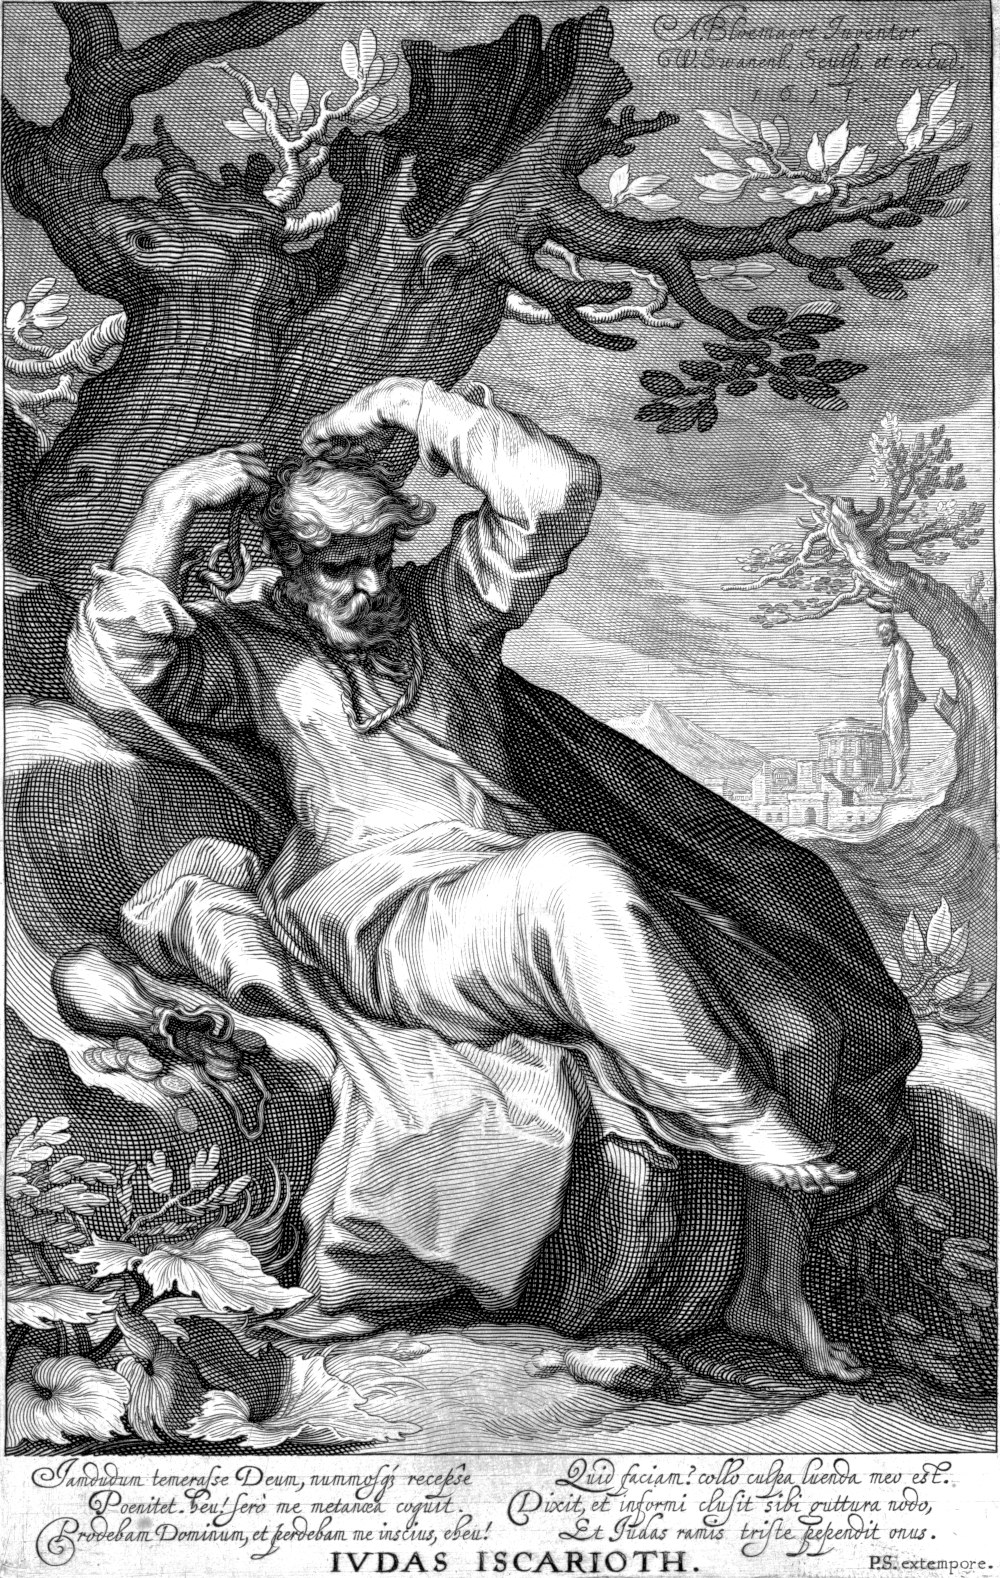
\includegraphics[keepaspectratio,width=0.4\textwidth]{figures/iudas-small.jpg}
  \caption{\citeart{IudasIscarioth}}
  \label{fig:iudas}
\end{figure}
\lettrine{T}{he} principal agent and procurer of this mischief is the devil; those
whom God forsakes, the devil by his permission lays hold on. Sometimes
he persecutes them with that worm of conscience, as he did Judas,
\authorfootnote{6694}Saul, and others. The poets call it Nemesis, but it is indeed
God's just judgment, sero sed serio, he strikes home at last, and
setteth upon them as a thief in the night, 1 Thes. ii. \authorfootnote{6695}This
temporary passion made David cry out, Lord, rebuke me not in thine
anger, neither chasten me in thine heavy displeasure; for thine arrows
have light upon me, \&c. there is nothing sound in my flesh, because of
thine anger. Again, I roar for the very grief of my heart: and Psalm
xxii. My God, my God, why hast thou forsaken me, and art so far from my
health, and the words of my crying? I am like to water poured out, my
bones are out of joint, mine heart is like wax, that is molten in the
midst of my bowels. So Psalm lxxxviii. 15 and 16 vers. and Psalm cii. I
am in misery at the point of death, from my youth I suffer thy terrors,
doubting for my life; thine indignations have gone over me, and thy
fear hath cut me off. Job doth often complain in this kind; and those
God doth not assist, the devil is ready to try and torment, still
seeking whom he may devour. If he find them merry, saith Gregory, he
tempts them forthwith to some dissolute act; if pensive and sad, to a
desperate end. Aut suadendo blanditur, aut minando terret, sometimes by
fair means, sometimes again by foul, as he perceives men severally
inclined. His ordinary engine by which he produceth this effect, is the
melancholy humour itself, which is balneum diaboli, the devil's bath;
and as in Saul, those evil spirits get in \authorfootnote{6696}as it were, and take
possession of us. Black choler is a shoeing-horn, a bait to allure
them, insomuch that many writers make melancholy an ordinary cause, and
a symptom of despair, for that such men are most apt, by reason of
their ill-disposed temper, to distrust, fear, grief, mistake, and
amplify whatsoever they preposterously conceive, or falsely apprehend.
Conscientia scrupulosa nascitur ex vitio naturali, complexione
melancholica (saith Navarrus cap. 27. num. 282. tom. 2. cas. conscien.)
The body works upon the mind, by obfuscating the spirits and corrupted
instruments, which \authorfootnote{6697}Perkins illustrates by simile of an artificer,
that hath a bad tool, his skill is good, ability correspondent, by
reason of ill tools his work must needs be lame and imperfect. But
melancholy and despair, though often, do not always concur; there is
much difference: melancholy fears without a cause, this upon great
occasion; melancholy is caused by fear and grief, but this torment
procures them and all extremity of bitterness; much melancholy is
without affliction of conscience, as \authorfootnote{6698}Bright and Perkins
illustrate by four reasons; and yet melancholy alone may be sometimes a
sufficient cause of this terror of conscience. \authorfootnote{6699}Felix Plater so
found it in his observations, e melancholicis alii damnatos se putant,
Deo curae, non sunt, nec praedestinati, \&c. They think they are not
predestinate, God hath forsaken them; and yet otherwise very zealous
and religious; and 'tis common to be seen, melancholy for fear of God's
judgment and hell-fire, drives men to desperation; fear and sorrow, if
they be immoderate, end often with it. Intolerable pain and anguish,
long sickness, captivity, misery, loss of goods, loss of friends, and
those lesser griefs, do sometimes effect it, or such dismal accidents.
Si non statim relevantur, \authorfootnote{6700}Mercennus, dubitant an sit Deus, if
they be not eased forthwith, they doubt whether there be any God, they
rave, curse, and are desperately mad because good men are oppressed,
wicked men flourish, they have not as they think to their desert, and
through impatience of calamities are so misaffected. Democritus put out
his eyes, ne malorum civium prosperos videret successus, because he
could not abide to see wicked men prosper, and was therefore ready to
make away himself, as \authorfootnote{6701}Agellius writes of him. Felix Plater hath a
memorable example in this kind, of a painter's wife in Basil, that was
melancholy for her son's death, and for melancholy became desperate;
she thought God would not pardon her sins, \authorfootnote{6702}and for four months
still raved, that she was in hell-fire, already damned. When the humour
is stirred up, every small object aggravates and incenseth it, as the
parties are addicted. \authorfootnote{6703}The same author hath an example of a
merchant man, that for the loss of a little wheat, which he had over
long kept, was troubled in conscience, for that he had not sold it
sooner, or given it to the poor, yet a good scholar and a great divine;
no persuasion would serve to the contrary, but that for this fact he
was damned: in other matters Very judicious and discreet. Solitariness,
much fasting, divine meditation, and contemplations of God's judgments,
most part accompany this melancholy, and are main causes, as
\authorfootnote{6704}Navarrus holds; to converse with such kinds of persons so
troubled, is sufficient occasion of trouble to some men. Nonnulli ob
longas inedias, studia et meditationes coelestes, de rebus sacris et
religione semper agitant, \&c. Many, (saith P. Forestus) through long
fasting, serious meditations of heavenly things, fall into such fits;
and as Lemnius adds, lib. 4. cap. 21, \authorfootnote{6705}If they be solitary given,
superstitious, precise, or very devout: seldom shall you find a
merchant, a soldier, an innkeeper, a bawd, a host, a usurer, so
troubled in mind, they have cheverel consciences that will stretch,
they are seldom moved in this kind or molested: young men and middle
age are more wild and less apprehensive; but old folks, most part, such
as are timorous and religiously given. Pet. Forestus observat. lib. 10.
cap. 12. de morbis cerebri, hath a fearful example of a minister, that
through precise fasting in Lent, and overmuch meditation, contracted
this mischief, and in the end became desperate, thought he saw devils
in his chamber, and that he could not be saved; he smelled nothing, as
he said, but fire and brimstone, was already in hell, and would ask
them, still, if they did not \authorfootnote{6706}smell as much. I told him he was
melancholy, but he laughed me to scorn, and replied that he saw devils,
talked with them in good earnest, Would spit in my face, and ask me if
1 did not smell brimstone, but at last he was by him cured. Such
another story I find in Plater observat. lib. 1. A poor fellow had done
some foul offence, and for fourteen days would eat no meat, in the end
became desperate, the divines about him could not ease him, \authorfootnote{6707}but
so he died. Continual meditation of God's judgments troubles many,
Multi ob timorem futuri judicii, saith Guatinerius cap. 5. tract. 15.
et suspicionem desperabundi sunt. David himself complains that God's
judgments terrified his soul, Psalm cxix. part. 16. vers. 8. My flesh
trembleth for fear of thee, and I am afraid of thy judgments. Quoties
diem illum cogito (saith \authorfootnote{6708}Hierome) toto corpore contremisco, I
tremble as often as I think of it. The terrible meditation of hell-fire
and eternal punishment much torments a sinful silly soul. What's a
thousand years to eternity? Ubi moeror, ubi fletus, ubi dolor
sempiternus. Mors sine morte, finis sine fine; a finger burnt by chance
we may not endure, the pain is so grievous, we may not abide an hour, a
night is intolerable; and what shall this unspeakable fire then be that
burns for ever, innumerable infinite millions of years, in omne aevum
in aeternum. O eternity!

\authorfootnote{6709}Aeternitas est illa vox,
Vox illa fulminatrix,

Tonitruis minacior,
Fragoribusque coeli,

Aeternitas est illa vox,
-meta carens et orta, \&c.

Tormenta nulla territant,
Quae finiuntur annis;

Aeternitas, aeternitas
Versat coquilque pectus.

Auget haec poenas indies,
Centuplicatque flammas, \&c.

This meditation terrifies these poor distressed souls, especially if
their bodies be predisposed by melancholy, they religiously given, and
have tender consciences, every small object affrights them, the very
inconsiderate reading of Scripture itself, and misinterpretation of
some places of it; as, Many are called, few are chosen. Not every one
that saith Lord. Fear not little flock. He that stands, let him take
heed lest he fall. Work out your salvation with fear and trembling,
That night two shall be in a bed, one received, the other left. Strait
is the way that leads to heaven, and few there are that enter therein.
The parable of the seed and of the sower, some fell on barren ground,
some was choked. Whom he hath predestinated he hath chosen. He will
have mercy on whom he will have mercy. Non est volentis nec currentis,
sed miserentis Dei. These and the like places terrify the souls of
many; election, predestination, reprobation, preposterously conceived,
offend divers, with a deal of foolish presumption, curiosity, needless
speculation, contemplation, solicitude, wherein they trouble and puzzle
themselves about those questions of grace, free will, perseverance,
God's secrets; they will know more than is revealed of God in his word,
human capacity, or ignorance can apprehend, and too importunate inquiry
after that which is revealed; mysteries, ceremonies, observation of
Sabbaths, laws, duties, \&c., with many such which the casuists discuss,
and schoolmen broach, which divers mistake, misconstrue, misapply to
themselves, to their own undoing, and so fall into this gulf. They
doubt of their election, how they shall know, it, by what signs. And so
far forth, saith Luther, with such nice points, torture and crucify
themselves, that they are almost mad, and all they get by it is this,
they lay open a gap to the devil by desperation to carry them to hell;
but the greatest harm of all proceeds from those thundering ministers,
a most frequent cause they are of this malady: \authorfootnote{6710}and do more harm
in the church (saith Erasmus) than they that flatter; great danger on
both sides, the one lulls them asleep in carnal security, the other
drives them to despair. Whereas, \authorfootnote{6711}St. Bernard well adviseth, We
should not meddle with the one without the other, nor speak of judgment
without mercy; the one alone brings desperation, the other security.
But these men are wholly for judgment; of a rigid disposition
themselves, there is no mercy with them, no salvation, no balsam for
their diseased souls, they can speak of nothing but reprobation,
hell-fire, and damnation; as they did Luke xi. 46. lade men with
burdens grievous to be borne, which they themselves touch not with a
finger. 'Tis familiar with our papists to terrify men's souls with
purgatory, tales, visions, apparitions, to daunt even the most generous
spirits, to \authorfootnote{6712}require charity, as Brentius observes, of others,
bounty, meekness, love, patience, when they themselves breathe nought
but lust, envy, covetousness. They teach others to fast, give alms, do
penance, and crucify their mind with superstitious observations, bread
and water, hair clothes, whips, and the like, when they themselves have
all the dainties the world can afford, lie on a down-bed with a
courtesan in their arms: Heu quantum patimur pro Christo, as \authorfootnote{6713}he
said, what a cruel tyranny is this, so to insult over and terrify men's
souls! Our indiscreet pastors many of them come not far behind, whilst
in their ordinary sermons they speak so much of election,
predestination, reprobation, ab aeterno, subtraction of grace,
preterition, voluntary permission, \&c., by what signs and tokens they
shall discern and try themselves, whether they be God's true children
elect, an sint reprobi, praedestinati, \&c., with such scrupulous
points, they still aggravate sin, thunder out God's judgments without
respect, intempestively rail at and pronounce them damned in all
auditories, for giving so much to sports and honest recreations, making
every small fault and thing indifferent an irremissible offence, they
so rent, tear and wound men's consciences, that they are almost mad,
and at their wits' end.
These bitter potions (saith \authorfootnote{6714}Erasmus) are still in their mouths,
nothing but gall and horror, and a mad noise, they make all their
auditors desperate: many are wounded by this means, and they commonly
that are most devout and precise, have been formerly presumptuous, and
certain of their salvation; they that have tender consciences, that
follow sermons, frequent lectures, that have indeed least cause, they
are most apt to mistake, and fall into these miseries. I have heard
some complain of Parson's Resolution, and other books of like nature
(good otherwise), they are too tragical, too much dejecting men,
aggravating offences: great care and choice, much discretion is
required in this kind.
The last and greatest cause of this malady, is our own conscience,
sense of our sins, and God's anger justly deserved, a guilty conscience
for some foul offence formerly committed,-\authorfootnote{6715}O miser Oreste, quid
morbi te perdit? Or: Conscientia, Sum enim mihi conscius de malis
perpetratis.\authorfootnote{6716} A good conscience is a continual feast, but a galled
conscience is as great a torment as can possibly happen, a still baking
oven, (so Pierius in his Hieroglyph, compares it) another hell. Our
conscience, which is a great ledger book, wherein are written all our
offences, a register to lay them up, (which those \authorfootnote{6717}Egyptians in
their hieroglyphics expressed by a mill, as well for the continuance,
as for the torture of it) grinds our souls with the remembrance of some
precedent sins, makes us reflect upon, accuse and condemn our own
selves. \authorfootnote{6718}Sin lies at door, \&c. I know there be many other causes
assigned by Zanchius, \authorfootnote{6719}Musculus, and the rest; as incredulity,
infidelity, presumption, ignorance, blindness, ingratitude, discontent,
those five grand miseries in Aristotle, ignominy, need, sickness,
enmity, death, \&c.; but this of conscience is the greatest,
\authorfootnote{6720}Instar ulceris corpus jugiter percellens: The scrupulous
conscience (as \authorfootnote{6721}Peter Forestus calls it) which tortures so many,
that either out of a deep apprehension of their unworthiness, and
consideration of their own dissolute life, accuse themselves and
aggravate every small offence, when there is no such cause, misdoubting
in the meantime God's mercies, they fall into these inconveniences. The
poet calls them \authorfootnote{6722}furies dire, but it is the conscience alone which
is a thousand witnesses to accuse us, \authorfootnote{6723} Nocte dieque suum gestant
in pectore testem. A continual tester to give in evidence, to empanel a
jury to examine us, to cry guilty, a persecutor with hue and cry to
follow, an apparitor to summon us, a bailiff to carry us, a serjeant to
arrest, an attorney to plead against us, a gaoler to torment, a judge
to condemn, still accusing, denouncing, torturing and molesting. And as
the statue of Juno in that holy city near Euphrates in \authorfootnote{6724}Assyria
will look still towards you, sit where you will in her temple, she
stares full upon you, if you go by, she follows with her eye, in all
sites, places, conventicles, actions, our conscience will be still
ready to accuse us. After many pleasant days, and fortunate adventures,
merry tides, this conscience at last doth arrest us. Well he may escape
temporal punishment, \authorfootnote{6725}bribe a corrupt judge, and avoid the censure
of law, and flourish for a time; for \authorfootnote{6726}who ever saw (saith
Chrysostom) a covetous man troubled in mind when he is telling of his
money, an adulterer mourn with his mistress in his arms? we are then
drunk with pleasure, and perceive nothing: yet as the prodigal son had
dainty fare, sweet music at first, merry company, jovial entertainment,
but a cruel reckoning in the end, as bitter as wormwood, a fearful
visitation commonly follows. And the devil that then told thee that it
was a light sin, or no sin at all, now aggravates on the other side,
and telleth thee, that it is a most irremissible offence, as he did by
Cain and Judas, to bring them to despair; every small circumstance
before neglected and contemned, will now amplify itself, rise up in
judgment, and accuse the dust of their shoes, dumb creatures, as to
Lucian's tyrant, lectus et candela, the bed and candle did bear
witness, to torment their souls for their sins past. Tragical examples
in this kind are too familiar and common: Adrian, Galba, Nero, Otho,
Vitellius, Caracalla, were in such horror of conscience for their
offences committed, murders, rapes, extortions, injuries, that they
were weary of their lives, and could get nobody to kill them.
\authorfootnote{6727}Kennetus, King of Scotland, when he had murdered his nephew
Malcom, King Duffe's son, Prince of Cumberland, and with counterfeit
tears and protestations dissembled the matter a long time, \authorfootnote{6728}at
last his conscience accused him, his unquiet soul could not rest day or
night, he was terrified with fearful dreams, visions, and so miserably
tormented all his life. It is strange to read what \authorfootnote{6729}Cominaeus hath
written of Louis XI. that French King; of Charles VIII.; of Alphonsus,
King of Naples; in the fury of his passion how he came into Sicily, and
what pranks he played. Guicciardini, a man most unapt to believe lies,
relates how that Ferdinand his father's ghost who before had died for
grief, came and told him, that he could not resist the French King, he
thought every man cried France, France; the reason of it (saith
Cominseus) was because he was a vile tyrant, a murderer, an oppressor
of his subjects, he bought up all commodities, and sold them at his own
price, sold abbeys to Jews and Falkoners; both Ferdinand his father,
and he himself never made conscience of any committed sin; and to
conclude, saith he, it was impossible to do worse than they did. Why
was Pausanias the Spartan tyrant, Nero, Otho, Galba, so persecuted with
spirits in every house they came, but for their murders which they had
committed? \authorfootnote{6730}Why doth the devil haunt many men's houses after their
deaths, appear to them living, and take possession of their
habitations, as it were, of their palaces, but because of their several
villainies? Why had Richard the Third such fearful dreams, saith
Polydore, but for his frequent murders? Why was Herod so tortured in
his mind? because he had made away Mariamne his wife. Why was
Theodoric, the King of the Goths, so suspicious, and so affrighted with
a fish head alone, but that he had murdered Symmachus, and Boethius his
son-in-law, those worthy Romans? Caelius, lib. 27. cap. 22. See more in
Plutarch, in his tract De his qui sero a Numine puniuntur, and in his
book De tranquillitate animi, \&c. Yea, and sometimes GOD himself hath a
hand in it, to show his power, humiliate, exercise, and to try their
faith, (divine temptation, Perkins calls it, Cas. cons. lib. 1. cap. 8.
sect. 1.) to punish them for their sins. God the avenger, as
\authorfootnote{6731}David terms him, ultor a tergo Deus, his wrath is apprehended of
a guilty, soul, as by Saul and Judas, which the poets expressed by
Adrastia, or Nemesis:
\authorfootnote{6732}Assequitur Nemesique virum vestigia servat,
Ne male quid facias.---

And she is, as \authorfootnote{6733}Ammianus, lib. 14. describes her, the queen of
causes, and moderator of things, now she pulls down the proud, now she
rears and encourageth those that are good; he gives instance in his
Eusebius; Nicephorus, lib. 10. cap. 35. eccles. hist. in Maximinus and
Julian. Fearful examples of God's just judgment, wrath and vengeance,
are to be found in all histories, of some that have been eaten to death
with rats and mice, as \authorfootnote{6734}Popelius, the second King of Poland, ann.
830, his wife and children; the like story is of Hatto, Archbishop of
Mentz, ann. 969, so devoured by these vermin, which howsoever Serrarius
the Jesuit Mogunt. rerum lib. 4. cap. 5. impugn by twenty-two
arguments, Tritemius, \authorfootnote{6735}Munster, Magdeburgenses, and many others
relate for a truth. Such another example I find in Geraldus Cambrensis
Itin. Cam. lib. 2. cap. 2. and where not?
And yet for all these terrors of conscience, affrighting punishments
which are so frequent, or whatsoever else may cause or aggravate this
fearful malady in other religions, I see no reason at all why a papist
at any time should despair, or be troubled for his sins; for let him be
never so dissolute a caitiff so notorious a villain, so monstrous a
sinner, out of that treasure of indulgences and merits of which the
pope is dispensator, he may have free pardon and plenary remission of
all his sins. There be so many general pardons for ages to come, forty
thousand years to come, so many jubilees, so frequent gaol-deliveries
out of purgatory for all souls, now living, or after dissolution of the
body, so many particular masses daily said in several churches, so many
altars consecrated to this purpose, that if a man have either money or
friends, or will take any pains to come to such an altar, hear a mass,
say so many paternosters, undergo such and such penance, he cannot do
amiss, it is impossible his mind should be troubled, or he have any
scruple to molest him. Besides that Taxa Camerae Apostolicae, which was
first published to get money in the days of Leo Decimus, that sharking
pope, and since divulged to the same ends, sets down such easy rates
and dispensations for all offences, for perjury, murder, incest,
adultery, \&c., for so many grosses or dollars (able to invite any man
to sin, and provoke him to offend, methinks, that otherwise would not)
such comfortable remission, so gentle and parable a pardon, so ready at
hand, with so small cost and suit obtained, that I cannot see how he
that hath any friends amongst them (as I say) or money in his purse, or
will at least to ease himself, can any way miscarry or be misaffected,
how he should be desperate, in danger of damnation, or troubled in
mind. Their ghostly fathers can so readily apply remedies, so cunningly
string and unstring, wind and unwind their devotions, play upon their
consciences with plausible speeches and terrible threats, for their
best advantage settle and remove, erect with such facility and deject,
let in and out, that I cannot perceive how any man amongst them should
much or often labour of this disease, or finally miscarry. The causes
above named must more frequently therefore take hold in others.

%SUBSECT. IV.-_Symptoms of Despair, Fear, Sorrow, Suspicion, Anxiety, Horror of Conscience, Fearful Dreams and Visions_.
\section[Symptoms of Despair]{Symptoms of Despair, Fear, Sorrow, Suspicion, Anxiety, Horror of Conscience, Fearful Dreams and Visions.}

\lettrine{A}{s} shoemakers do when they bring home shoes, still cry leather is
dearer and dearer, may I justly say of those melancholy symptoms: these
of despair are most violent, tragical, and grievous, far beyond the
rest, not to be expressed but negatively, as it is privation of all
happiness, not to be endured; for a wounded spirit who can bear it?
Prov. xviii. 19. What, therefore, \authorfootnote{6736}Timanthes did in his picture of
Iphigenia, now ready to be sacrificed, when he had painted Chalcas
mourning, Ulysses sad, but most sorrowful Menelaus; and showed all his
art in expressing a variety of affections, he covered the maid's father
Agamemnon's head with a veil, and left it to every spectator to
conceive what he would himself; for that true passion and sorrow in
summo gradu, such as his was, could not by any art be deciphered. What
he did in his picture, I will do in describing the symptoms of despair;
imagine what thou canst, fear, sorrow, furies, grief, pain, terror,
anger, dismal, ghastly, tedious, irksome, \&c. it is not sufficient, it
comes far short, no tongue can tell, no heart conceive it. 'Tis an
epitome of hell, an extract, a quintessence, a compound, a mixture of
all feral maladies, tyrannical tortures, plagues, and perplexities.
There is no sickness almost but physic provideth a remedy for it; to
every sore chirurgery will provide a slave; friendship helps poverty;
hope of liberty easeth imprisonment; suit and favour revoke banishment;
authority and time wear away reproach: but what physic, what
chirurgery, what wealth, favour, authority can relieve, bear out,
assuage, or expel a troubled conscience? A quiet mind cureth all them,
but all they cannot comfort a distressed soul: who can put to silence
the voice of desperation? All that is single in other melancholy,
Horribile, dirum, pestilens, atrox, ferum, concur in this, it is more
than melancholy in the highest degree; a burning fever of the soul; so
mad, saith \authorfootnote{6737}Jacchinus, by this misery; fear, sorrow, and despair,
he puts for ordinary symptoms of melancholy. They are in great pain and
horror of mind, distraction of soul, restless, full of continual fears,
cares, torments, anxieties, they can neither eat, drink, nor sleep for
them, take no rest,
\authorfootnote{6738}Perpetua impietas, nec mensae tempore cessat,
Exagitat vesana quies, somnique furentes.

Neither at bed, nor yet at board,
Will any rest despair afford.

Fear takes away their content, and dries the blood, wasteth the marrow,
alters their countenance, even in their greatest delights, singing,
dancing, dalliance, they are still (saith \authorfootnote{6739}Lemnius) tortured in
their souls. It consumes them to nought, I am like a pelican in the
wilderness (saith David of himself, temporally afflicted), an owl,
because of thine indignation, Psalm cii. 8, 10, and Psalm lv. 4. My
heart trembleth within me, and the terrors of death have come upon me;
fear and trembling are come upon me, \&c. at death's door, Psalm cvii.
18. Their soul abhors all manner of meats. Their \authorfootnote{6740}sleep is (if it
be any) unquiet, subject to fearful dreams and terrors. Peter in his
bonds slept secure, for he knew God protected him; and Tully makes it
an argument of Roscius Amerinus' innocency, that he killed not his
father, because he so securely slept. Those martyrs in the primitive
church were most \authorfootnote{6741}cheerful and merry in the midst of their
persecutions; but it is far otherwise with these men, tossed in a sea,
and that continually without rest or intermission, they can think of
nought that is pleasant, \authorfootnote{6742}their conscience will not let them be
quiet, in perpetual fear, anxiety, if they be not yet apprehended, they
are in doubt still they shall be ready to betray themselves, as Cain
did, he thinks every man will kill him; and roar for the grief of
heart, Psalm xxxviii. 8, as David did; as Job did, xx. 3, 21, 22, \&c.,
Wherefore is light given to him that is in misery, and life to them
that have heavy hearts? which long for death, and if it come not,
search it more than treasures, and rejoice when they can find the
grave. They are generally weary of their lives, a trembling heart they
have, a sorrowful mind, and little or no rest. Terror ubique tremor,
timor undique et undique terror. Fears, terrors, and affrights in all
places, at all times and seasons. Cibum et potum pertinaciter
aversantur multi, nodum in scirpo quaeritantes, et culpam imaginantes
ubi nulla est, as Wierus writes de Lamiis lib. 3. c. 7. they refuse
many of them meat and drink, cannot rest, aggravating still and
supposing grievous offences where there are none. God's heavy wrath is
kindled in their souls, and notwithstanding their continual prayers and
supplications to Christ Jesus, they have no release or ease at all, but
a most intolerable torment, and insufferable anguish of conscience, and
that makes them, through impatience, to murmur against God many times,
to rave, to blaspheme, turn atheists, and seek to offer violence to
themselves. Deut. xxviii. 65, 68. In the morning they wish for evening,
and for morning in the evening, for the sight of their eyes which they
see, and fear of hearts. \authorfootnote{6743}Marinus Mercennus, in his comment on
Genesis, makes mention of a desperate friend of his, whom, amongst
others, he came to visit, and exhort to patience, that broke out into
most blasphemous atheistical speeches, too fearful to relate, when they
wished him to trust in God, Quis est ille Deus (inquit) ut serviam
illi, quid proderit si oraverim; si praesens est, cur non succurrit?
cur non me carcere, inertia, squalore confectum liberat? quid ego feci?
\&c. absit a me hujusmodi Deus. Another of his acquaintance broke out
into like atheistical blasphemies, upon his wife's death raved, cursed,
said and did he cared not what. And so for the most part it is with
them all, many of them, in their extremity, think they hear and see
visions, outcries, confer with devils, that they are tormented,
possessed, and in hell-fire, already damned, quite forsaken of God,
they have no sense or feeling of mercy, or grace, hope of salvation,
their sentence of condemnation is already past, and not to be revoked,
the devil will certainly have them. Never was any living creature in
such torment before, in such a miserable estate, in such distress of
mind, no hope, no faith, past cure, reprobate, continually tempted to
make away themselves. Something talks with them, they spit fire and
brimstone, they cannot but blaspheme, they cannot repent, believe or
think a good thought, so far carried; ut cogantur ad impia cogitandum
etiam contra voluntatem, said \authorfootnote{6744}Felix Plater, ad blasphemiam erga
deum, ad multa horrenda perpetranda, ad manus violentas sibi
inferendas, \&c., and in their distracted fits and desperate humours, to
offer violence to others, their familiar and dear friends sometimes, or
to mere strangers, upon very small or no occasion; for he that cares
not for his own, is master of another man's life. They think evil
against their wills; that which they abhor themselves, they must needs
think, do, and speak. He gives instance in a patient of his, that when
he would pray, had such evil thoughts still suggested to him, and
wicked \authorfootnote{6745}meditations. Another instance he hath of a woman that was
often tempted to curse God, to blaspheme and kill herself. Sometimes
the devil (as they say) stands without and talks with them, sometimes
he is within them, as they think, and there speaks and talks as to such
as are possessed: so Apollodorus, in Plutarch, thought his heart spake
within him. There is a most memorable example of \authorfootnote{6746}Francis Spira,
an advocate of Padua, Ann. 1545, that being desperate, by no counsel of
learned men could be comforted: he felt (as he said) the pains of hell
in his soul; in all other things he discoursed aright, but in this most
mad. Frismelica, Bullovat, and some other excellent physicians, could
neither make him eat, drink, or sleep, no persuasion could ease him.
Never pleaded any man so well for himself, as this man did against
himself, and so he desperately died. Springer, a lawyer, hath written
his life. Cardinal Crescence died so likewise desperate at Verona,
still he thought a black dog followed him to his death-bed, no man
could drive the dog away, Sleiden. com. 23. cap. lib. 3. Whilst I was
writing this Treatise, saith Montaltus, cap. 2. de mel. \authorfootnote{6747}A nun
came to me for help, well for all other matters, but troubled in
conscience for five years last past; she is almost mad, and not able to
resist, thinks she hath offended God, and is certainly damned. Felix
Plater hath store of instances of such as thought themselves damned,
\authorfootnote{6748} forsaken of God, \&c. One amongst the rest, that durst not go to
church, or come near the Rhine, for fear to make away himself, because
then he was most especially tempted. These and such like symptoms are
intended and remitted, as the malady itself is more or less; some will
hear good counsel, some will not; some desire help, some reject all,
and will not be eased.

%SUBSECT. V.-_Prognostics of Despair, Atheism, Blasphemy, violent death, &c._
\section[Prognostics of Despair]{Prognostics of Despair, Atheism, Blasphemy, violent death, \&c.}

\lettrine{M}{ost} part these kind of persons make \authorfootnote{6749}away themselves, some are
mad, blaspheme, curse, deny God, but most offer violence to their own
persons, and sometimes to others. A wounded spirit who can bear? Prov.
xviii. 14. As Cain, Saul, Achitophel, Judas, blasphemed and died. Bede
saith, Pilate died desperate eight years after Christ. \authorfootnote{6750}Felix
Plater hath collected many examples. \authorfootnote{6751}A merchant's wife that was
long troubled with such temptations, in the night rose from her bed,
and out of the window broke her neck into the street: another drowned
himself desperate as he was in the Rhine: some cut their throats, many
hang themselves. But this needs no illustration. It is controverted by
some, whether a man so offering violence to himself, dying desperate,
may be saved, ay or no? If they die so obstinately and suddenly, that
they cannot so much as wish for mercy, the worst is to be suspected,
because they die impenitent. \authorfootnote{6752}If their death had been a little
more lingering, wherein they might have some leisure in their hearts to
cry for mercy, charity may judge the best; divers have been recovered
out of the very act of hanging and drowning themselves, and so brought
ad sanam mentem, they have been very penitent, much abhorred their
former act, confessed that they have repented in an instant, and cried
for mercy in their hearts. If a man put desperate hands upon himself,
by occasion of madness or melancholy, if he have given testimony before
of his regeneration, in regard he doth this not so much out of his
will, as ex vi morbi, we must make the best construction of it, as
\authorfootnote{6753}Turks do, that think all fools and madmen go directly to heaven.

%SUBSECT. VI.-_Cure of Despair by Physic, Good Counsel, Comforts, \&c._
\section[Cure of Despair]{Cure of Despair by Physic, Good Counsel, Comforts, \&c.}

\lettrine{E}{xperience} teacheth us, that though many die obstinate and wilful in
this malady, yet multitudes again are able to resist and overcome, seek
for help and find comfort, are taken e faucibus Erebi, from the chops
of hell, and out of the devil's paws, though they have by
\authorfootnote{6754}obligation, given themselves to him. Some out of their own
strength, and God's assistance, Though He kill me, (saith Job,) yet
will I trust in Him, out of good counsel, advice and physic.
\authorfootnote{6755}Bellovacus cured a monk by altering his habit, and course of
life: Plater many by physic alone. But for the most part they must
concur; and they take a wrong course that think to overcome this feral
passion by sole physic; and they are as much out, that think to work
this effect by good service alone, though both be forcible in
themselves, yet vis unita fortior, they must go hand in hand to this
disease:-alterius sic altera poscit opem. For physic the like course is
to be taken with this as in other melancholy: diet, air, exercise, all
those passions and perturbations of the mind, \&c. are to be rectified
by the same means. They must not be left solitary, or to themselves,
never idle, never out of company. Counsel, good comfort is to be
applied, as they shall see the parties inclined, or to the causes,
whether it be loss, fear, be grief, discontent, or some such feral
accident, a guilty conscience, or otherwise by frequent meditation, too
grievous an apprehension, and consideration of his former life; by
hearing, reading of Scriptures, good divines, good advice and
conference, applying God's word to their distressed souls, it must be
corrected and counterpoised. Many excellent exhortations, phraenetical
discourses, are extant to this purpose, for such as are any way
troubled in mind: Perkins, Greenham, Hayward, Bright, Abernethy,
Bolton, Culmannus, Helmingius, Caelius Secundus, Nicholas Laurentius,
are copious on this subject: Azorius, Navarrus, Sayrus, \&c., and such
as have written cases of conscience amongst our pontifical writers. But
because these men's works are not to all parties at hand, so parable at
all times, I will for the benefit and ease of such as are afflicted, at
the request of some \authorfootnote{6756}friends, recollect out of their voluminous
treatises, some few such comfortable speeches, exhortations, arguments,
advice, tending to this subject, and out of God's word, knowing, as
Culmannus saith upon the like occasion, \authorfootnote{6757}how unavailable and vain
men's councils are to comfort an afflicted conscience, except God's
word concur and be annexed, from which comes life, ease, repentance,
\&c. Presupposing first that which Beza, Greenham, Perkins, Bolton, give
in charge, the parties to whom counsel is given be sufficiently
prepared, humbled for their sins, fit for comfort, confessed, tried how
they are more or less afflicted, how they stand affected, or capable of
good advice, before any remedies be applied: to such therefore as are
so thoroughly searched and examined, I address this following
discourse.
Two main antidotes, \authorfootnote{6758}Hemmingius observes, opposite to despair,
good hope out of God's word, to be embraced; perverse security and
presumption from the devil's treachery, to be rejected; Illa solus
animae, haec pestis; one saves, the other kills, occidit animam, saith
Austin, and doth as much harm as despair itself, \authorfootnote{6759}Navarrus the
casuist reckons up ten special cures out of Anton. 1. part. Tit. 3.
cap. 10. 1. God. 2. Physic. 3. \authorfootnote{6760}Avoiding such objects as have
caused it. 4. Submission of himself to other men's judgments. 5. Answer
of all objections, \&c. All which Cajetan, Gerson, lib. de vit. spirit.
Sayrus, lib. 1. cons. cap. 14. repeat and approve out of Emanuel
Roderiques, cap. 51 et 52. Greenham prescribes six special rules,
Culmannus seven. First, to acknowledge all help come from God. 2. That
the cause of their present misery is sin. 3. To repent and be heartily
sorry for their sins. 4. To pray earnestly to God they may be eased. 5.
To expect and implore the prayers of the church, and good men's advice.
6. Physic. 7. To commend themselves to God, and rely upon His mercy:
others, otherwise, but all to this effect. But forasmuch as most men in
this malady are spiritually sick, void of reason almost, overborne by
their miseries, and too deep an apprehension of their sins, they cannot
apply themselves to good counsel, pray, believe, repent, we must, as
much as in us lies, occur and help their peculiar infirmities,
according to their several causes and symptoms, as we shall find them
distressed and complain.
The main matter which terrifies and torments most that are troubled in
mind, is the enormity of their offences, the intolerable burthen of
their sins, God's heavy wrath and displeasure so deeply apprehended,
that they account themselves reprobates, quite forsaken of God, already
damned, past all hope of grace, incapable of mercy, diaboli mancipia,
slaves of sin, and their offences so great they cannot be forgiven. But
these men must know there is no sin so heinous which is not pardonable
in itself, no crime so great but by God's mercy it may be forgiven.
Where sin aboundeth, grace aboundeth much more, Rom. v. 20. And what
the Lord said unto Paul in his extremity, 2 Cor. xi. 9. My grace is
sufficient for thee, for my power is made perfect through weakness:
concerns every man in like case. His promises are made indefinite to
all believers, generally spoken to all touching remission of sins that
are truly penitent, grieved for their offences, and desire to be
reconciled, Matt. ix. 12, 13, I came not to call the righteous but
sinners to repentance, that is, such as are truly touched in conscience
for their sins. Again, Matt. xi. 28, Come unto me all ye that are heavy
laden, and I will ease you. Ezek. xviii. 27, At what time soever a
sinner shall repent him of his sins from the bottom of his heart, I
will blot out all his wickedness out of my remembrance saith the Lord.
Isaiah xliii. 25, I, even I, am He that put away thine iniquity for
mine own sake, and will not remember thy sins. As a father (saith David
Psal. ciii. 13) hath compassion on his children, so hath the Lord
compassion on them that fear him. And will receive them again as the
prodigal son was entertained, Luke xv., if they shall so come with
tears in their eyes, and a penitent heart. Peccator agnoscat, Deus
ignoscit. The Lord is full of compassion and mercy, slow to anger, of
great kindness, Psal. ciii. 8. He will not always chide, neither keep
His anger for ever, 9. As high as the heaven is above the earth, so
great is His mercy towards them that fear Him, 11. As far as the East
is from the West, so far hath He removed our sins from us, 12. Though
Cain cry out in the anguish of his soul, my punishment is greater than
I can bear, 'tis not so; thou liest, Cain (saith Austin), God's mercy
is greater than thy sins. His mercy is above all His works, Psal. cxlv.
9, able to satisfy for all men's sins, antilutron, 1 Tim. ii. 6. His
mercy is a panacea, a balsam for an afflicted soul, a sovereign
medicine, an alexipharmacum for all sins, a charm for the devil; his
mercy was great to Solomon, to Manasseh, to Peter, great to all
offenders, and whosoever thou art, it may be so to thee. For why should
God bid us pray (as Austin infers) Deliver us from all evil, nisi ipse
misericors perseveraret, if He did not intend to help us? He therefore
that \authorfootnote{6761}doubts of the remission of his sins, denies God's mercy, and
doth Him injury, saith Austin. Yea, but thou repliest, I am a notorious
sinner, mine offences are not so great as infinite. Hear Fulgentius,
\authorfootnote{6762}God's invincible goodness cannot be overcome by sin, His infinite
mercy cannot be terminated by any: the multitude of His mercy is
equivalent to His magnitude. Hear \authorfootnote{6763}Chrysostom, Thy malice may be
measured, but God's mercy cannot be defined; thy malice is
circumscribed, His mercies infinite. As a drop of water is to the sea,
so are thy misdeeds to His mercy: nay, there is no such proportion to
be given; for the sea, though great, yet may be measured, but God's
mercy cannot be circumscribed. Whatsoever thy sins be then in quantity
or quality, multitude or magnitude, fear them not, distrust not. I
speak not this, saith \authorfootnote{6764}Chrysostom, to make thee secure and
negligent, but to cheer thee up. Yea but, thou urgest again, I have
little comfort of this which is said, it concerns me not: Inanis
poenitentia quam sequens culpa coinquinat, 'tis to no purpose for me to
repent, and to do worse than ever I did before, to persevere in sin,
and to return to my lusts as a dog to his vomit, or a swine to the
mire: \authorfootnote{6765}to what end is it to ask forgiveness of my sins, and yet
daily to sin again and again, to do evil out of a habit? I daily and
hourly offend in thought, word, and deed, in a relapse by mine own
weakness and wilfulness: my bonus genius, my good protecting angel is
gone, I am fallen from that I was or would be, worse and worse, my
latter end is worse than my beginning: Si quotidiae peccas, quotidie,
saith Chrysostom, poenitentiam age, if thou daily offend, daily repent:
\authorfootnote{6766}if twice, thrice, a hundred, a hundred thousand times, twice,
thrice, a hundred thousand times repent. As they do by an old house
that is out of repair, still mend some part or other; so do by thy
soul, still reform some vice, repair it by repentance, call to Him for
grace, and thou shalt have it; For we are freely justified by His
grace, Rom. iii. 24. If thine enemy repent, as our Saviour enjoined
Peter, forgive him seventy-seven times; and why shouldst thou think God
will not forgive thee? Why should the enormity of thy sins trouble
thee? God can do it, he will do it. My conscience (saith \authorfootnote{6767}Anselm)
dictates to me that I deserve damnation, my repentance will not suffice
for satisfaction: but thy mercy, O Lord, quite overcometh all my
transgressions. The gods once (as the poets feign) with a gold chain
would pull Jupiter out of heaven, but all they together could not stir
him, and yet he could draw and turn them as he would himself; maugre
all the force and fury of these infernal fiends, and crying sins, His
grace is sufficient. Confer the debt and the payment; Christ and Adam;
sin, and the cure of it; the disease and the medicine; confer the sick
man to his physician, and thou shalt soon perceive that his power is
infinitely beyond it. God is better able, as \authorfootnote{6768}Bernard informeth
us, to help, than sin to do us hurt; Christ is better able to save,
than the devil to destroy. \authorfootnote{6769}If he be a skilful Physician, as
Fulgentius adds, he can cure all diseases; if merciful, he will. Non
est perfecta bonitas a qua non omnis malitia vincitur, His goodness is
not absolute and perfect, if it be not able to overcome all malice.
Submit thyself unto Him, as St. Austin adviseth, \authorfootnote{6770}He knoweth best
what he doth; and be not so much pleased when he sustains thee, as
patient when he corrects thee; he is omnipotent, and can cure all
diseases when he sees his own time. He looks down from heaven upon
earth, that he may hear the mourning of prisoners, and deliver the
children of death, Psal. cii. 19. 20. And though our sins be as red as
scarlet, He can make them as white as snow, Isai. i. 18. Doubt not of
this, or ask how it shall be done: He is all-sufficient that promiseth;
qui fecit mundum de immundo, saith Chrysostom, he that made a fair
world of nought, can do this and much more for his part: do thou only
believe, trust in him, rely on him, be penitent and heartily sorry for
thy sins. Repentance is a sovereign remedy for all sins, a spiritual
wing to rear us, a charm for our miseries, a protecting amulet to expel
sin's venom, an attractive loadstone to draw God's mercy and graces
unto us. \authorfootnote{6771}Peccatum vulnus, poenitentia medicinam: sin made the
breach, repentance must help it; howsoever thine offence came, by
error, sloth, obstinacy, ignorance, exitur per poenitentiam, this is
the sole means to be relieved. \authorfootnote{6772}Hence comes our hope of safety, by
this alone sinners are saved, God is provoked to mercy. This unlooseth
all that is bound, enlighteneth darkness, mends that is broken, puts
life to that which was desperately dying: makes no respect of offences,
or of persons. \authorfootnote{6773}This doth not repel a fornicator, reject a
drunkard, resist a proud fellow, turn away an idolater, but entertains
all, communicates itself to all. Who persecuted the church more than
Paul, offended more than Peter? and yet by repentance (saith
Curysologus) they got both Magisterium et ministerium sanctitatis, the
Magistery of holiness. The prodigal son went far, but by repentance he
came home at last. \authorfootnote{6774}This alone will turn a wolf into a sheep, make
a publican a preacher, turn a thorn into an olive, make a debauched
fellow religious, a blasphemer sing halleluja, make Alexander the
coppersmith truly devout, make a devil a saint. \authorfootnote{6775}And him that
polluted his mouth with calumnies, lying, swearing, and filthy tunes
and tones, to purge his throat with divine Psalms. Repentance will
effect prodigious cures, make a stupend metamorphosis. A hawk came into
the ark, and went out again a hawk; a lion came in, went out a lion; a
bear, a bear; a wolf, a wolf; but if a hawk came into this sacred
temple of repentance, he will go forth a dove (saith \authorfootnote{6776}Chrysostom),
a wolf go out a sheep, a lion a lamb. \authorfootnote{6777}This gives sight to the
blind, legs to the lame, cures all diseases, confers grace, expels
vice, inserts virtue, comforts and fortifies the soul. Shall I say, let
thy sin be what it will, do but repent, it is sufficient. \authorfootnote{6778}Quem
poenitet peccasse pene est innocens. 'Tis true indeed and
all-sufficient this, they do confess, if they could repent; but they
are obdurate, they have cauterised consciences, they are in a reprobate
sense, they cannot think a good thought, they cannot hope for grace,
pray, believe, repent, or be sorry for their sins, they find no grief
for sin in themselves, but rather a delight, no groaning of spirit, but
are carried headlong to their own destruction, heaping wrath to
themselves against the day of wrath, Rom. ii. 5. 'Tis a grievous case
this I do yield, and yet not to be despaired; God of his bounty and
mercy calls all to repentance, Rom. ii. 4, thou mayst be called at
length, restored, taken to His grace, as the thief upon the cross, at
the last hour, as Mary Magdalene and many other sinners have been, that
were buried in sin. God (saith \authorfootnote{6779}Fulgentius) is delighted in the
conversion of a sinner, he sets no time; prolixitas temporis Deo non
praejudicat, aut gravitas peccati, deferring of time or grievousness of
sin, do not prejudicate his grace, things past and to come are all one
to Him, as present: 'tis never too late to repent. \authorfootnote{6780}This heaven of
repentance is still open for all distressed souls; and howsoever as yet
no signs appear, thou mayst repent in good time. Hear a comfortable
speech of St. Austin, \authorfootnote{6781}Whatsoever thou shall do, how great a
sinner soever, thou art yet living; if God would not help thee, he
would surely take thee away; but in sparing thy life, he gives thee
leisure, and invites thee to repentance. Howsoever as yet, I say, thou
perceivest no fruit, no feeling, findest no likelihood of it in
thyself, patiently abide the Lord's good leisure, despair not, or think
thou art a reprobate; He came to call sinners to repentance, Luke v.
32, of which number thou art one; He came to call thee, and in his time
will surely call thee. And although as yet thou hast no inclination to
pray, to repent, thy faith be cold and dead, and thou wholly averse
from all Divine functions, yet it may revive, as trees are dead in
winter, but flourish in the spring! these virtues may lie hid in thee
for the present, yet hereafter show themselves, and peradventure
already bud, howsoever thou dost not perceive. 'Tis Satan's policy to
plead against, suppress and aggravate, to conceal those sparks of faith
in thee. Thou dost not believe, thou sayest, yet thou wouldst believe
if thou couldst, 'tis thy desire to believe; then pray, \authorfootnote{6782}Lord help
mine unbelief: and hereafter thou shall certainly believe:
\authorfootnote{6783}Dabitur sitienti, it shall be given to him that thirsteth. Thou
canst not yet repent, hereafter thou shall; a black cloud of sin as yet
obnubilates thy soul, terrifies thy conscience, but this cloud may
conceive a rainbow at the last, and be quite dissipated by repentance.
Be of good cheer; a child is rational in power, not in act; and so art
thou penitent in affection, though not yet in action. 'Tis thy desire
to please God, to be heartily sorry; comfort thyself, no time is
overpast, 'tis never too late. A desire to repent is repentance itself,
though not in nature, yet in God's acceptance; a willing mind is
sufficient. Blessed are they that hunger and thirst after
righteousness, Matt. v. 6. He that is destitute of God's grace, and
wisheth for it, shall have it. The Lord (saith David, Psal. x. 17) will
hear the desire of the poor, that is, such as are in distress of body
and mind. 'Tis true thou canst not as yet grieve for thy sin, thou hast
no feeling of faith, I yield; yet canst thou grieve thou dost not
grieve? It troubles thee, I am sure, thine heart should be so
impenitent and hard, thou wouldst have it otherwise; 'tis thy desire to
grieve, to repent, and to believe. Thou lovest God's children and
saints in the meantime, hatest them not, persecutest them not, but
rather wishest thyself a true professor, to be as they are, as thou
thyself hast been heretofore; which is an evident token thou art in no
such desperate case. 'Tis a good sign of thy conversion, thy sins are
pardonable, thou art, or shalt surely be reconciled. The Lord is near
them that are of a contrite heart, Luke iv. 18. \authorfootnote{6784}A true desire of
mercy in the want of mercy, is mercy itself; a desire of grace in the
want of grace, is grace itself; a constant and earnest desire to
believe, repent, and to be reconciled to God, if it be in a touched
heart, is an acceptation of God, a reconciliation, faith and repentance
itself. For it is not thy faith and repentance, as \authorfootnote{6785}Chrysostom
truly teacheth, that is available, but God's mercy that is annexed to
it, He accepts the will for the deed: so that I conclude, to feel in
ourselves the want of grace, and to be grieved for it, is grace itself.
I am troubled with fear my sins are not forgiven, Careless objects: but
Bradford answers they are; For God hath given thee a penitent and
believing heart, that is, a heart which desireth to repent and believe;
for such an one is taken of him (he accepting the will for the deed)
for a truly penitent and believing heart.
All this is true thou repliest, but yet it concerns not thee, 'tis
verified in ordinary offenders, in common sins, but thine are of a
higher strain, even against the Holy Ghost himself, irremissible sins,
sins of the first magnitude, written with a pen of iron, engraven with
a point of a diamond. Thou art worse than a pagan, infidel, Jew, or
Turk, for thou art an apostate and more, thou hast voluntarily
blasphemed, renounced God and all religion, thou art worse than Judas
himself, or they that crucified Christ: for they did offend out of
ignorance, but thou hast thought in thine heart there is no God. Thou
hast given thy soul to the devil, as witches and conjurors do,
explicite and implicite, by compact, band and obligation (a desperate,
a fearful case) to satisfy thy lust, or to be revenged of thine
enemies, thou didst never pray, come to church, hear, read, or do any
divine duties with any devotion, but for formality and fashion's sake,
with a kind of reluctance, 'twas troublesome and painful to thee to
perform any such thing, praeter voluntatem, against thy will. Thou
never mad'st any conscience of lying, swearing, bearing false witness,
murder, adultery, bribery, oppression, theft, drunkenness, idolatry,
but hast ever done all duties for fear of punishment, as they were most
advantageous, and to thine own ends, and committed all such notorious
sins, with an extraordinary delight, hating that thou shouldst love,
and loving that thou shouldst hate. Instead of faith, fear and love of
God, repentance, \&c., blasphemous thoughts have been ever harboured in
his mind, even against God himself, the blessed Trinity; the
\authorfootnote{6786}Scripture false, rude, harsh, immethodical: heaven, hell,
resurrection, mere toys and fables, \authorfootnote{6787}incredible, impossible,
absurd, vain, ill contrived; religion, policy, and human invention, to
keep men in obedience, or for profit, invented by priests and lawgivers
to that purpose. If there be any such supreme power, he takes no notice
of our doings, hears not our prayers, regardeth them not, will not,
cannot help, or else he is partial, an excepter of persons, author of
sin, a cruel, a destructive God, to create our souls, and destinate
them to eternal damnation, to make us worse than our dogs and horses,
why doth he not govern things better, protect good men, root out wicked
livers? why do they prosper and flourish? as she raved in the
\authorfootnote{6788}tragedy-pellices caelum tenent, there they shine, Suasque Perseus
aureas stellas habet, where is his providence? how appears it?
\authorfootnote{6789}Marmoreo Licinus tumulo jacet, at Cato parvo,
Pomponius nullo, quis putet esse Deos.

Why doth he suffer Turks to overcome Christians, the enemy to triumph
over his church, paganism to domineer in all places as it doth,
heresies to multiply, such enormities to be committed, and so many such
bloody wars, murders, massacres, plagues, feral diseases! why doth he
not make us all good, able, sound? why makes he \authorfootnote{6790}venomous
creatures, rocks, sands, deserts, this earth itself the muck-hill of
the world, a prison, a house of correction? \authorfootnote{6791}Mentimur regnare
Jovem, \&c., with many such horrible and execrable conceits, not fit to
be uttered; Terribilia de fide, horribilia de Divinitate. They cannot
some of them but think evil, they are compelled volentes nolentes, to
blaspheme, especially when they come to church and pray, read, \&c.,
such foul and prodigious suggestions come into their hearts.
These are abominable, unspeakable offences, and most opposite to God,
tentationes foedae, et impiae, yet in this case, he or they that shall
be tempted and so affected, must know, that no man living is free from
such thoughts in part, or at some times, the most divine spirits have
been so tempted in some sort, evil custom, omission of holy exercises,
ill company, idleness, solitariness, melancholy, or depraved nature,
and the devil is still ready to corrupt, trouble, and divert our souls,
to suggest such blasphemous thoughts into our fantasies, ungodly,
profane, monstrous and wicked conceits: If they come from Satan, they
are more speedy, fearful and violent, the parties cannot avoid them:
they are more frequent, I say, and monstrous when they come; for the
devil he is a spirit, and hath means and opportunities to mingle
himself with our spirits, and sometimes more slyly, sometimes more
abruptly and openly, to suggest such devilish thoughts into our hearts;
he insults and domineers in melancholy distempered fantasies and
persons especially; melancholy is balneum, diaboli, as Serapio holds,
the devil's bath, and invites him to come to it. As a sick man frets,
raves in his fits, speaks and doth he knows not what, the devil
violently compels such crazed souls to think such damned thoughts
against their wills, they cannot but do it; sometimes more continuate,
or by fits, he takes his advantage, as the subject is less able to
resist, he aggravates, extenuates, affirms, denies, damns, confounds
the spirits, troubles heart, brain, humours, organs, senses, and wholly
domineers in their imaginations. If they proceed from themselves, such
thoughts, they are remiss and moderate, not so violent and monstrous,
not so frequent. The devil commonly suggests things opposite to nature,
opposite to God and his word, impious, absurd, such as a man would
never of himself, or could not conceive, they strike terror and horror
into the parties' own hearts. For if he or they be asked whether they
do approve of such like thoughts or no, they answer (and their own
souls truly dictate as much) they abhor them as much as hell and the
devil himself, they would fain think otherwise if they could; he hath
thought otherwise, and with all his soul desires so to think again; he
doth resist, and hath some good motions intermixed now and then: so
that such blasphemous, impious, unclean thoughts, are not his own, but
the devil's; they proceed not from him, but from a crazed phantasy,
distempered humours, black fumes which offend his brain: \authorfootnote{6792}they are
thy crosses, the devil's sins, and he shall answer for them, he doth
enforce thee to do that which thou dost abhor, and didst never give
consent to: and although he hath sometimes so slyly set upon thee, and
so far prevailed, as to make thee in some sort to assent to such wicked
thoughts, to delight in, yet they have not proceeded from a confirmed
will in thee, but are of that nature which thou dost afterwards reject
and abhor. Therefore be not overmuch troubled and dismayed with such
kind of suggestions, at least if they please thee not, because they are
not thy personal sins, for which thou shalt incur the wrath of God, or
his displeasure: contemn, neglect them, let them go as they come,
strive not too violently, or trouble thyself too much, but as our
Saviour said to Satan in like case, say thou, avoid Satan, I detest
thee and them. Satanae est mala ingerere (saith Austin) nostrum non
consentire: as Satan labours to suggest, so must we strive not to give
consent, and it will be sufficient: the more anxious and solicitous
thou art, the more perplexed, the more thou shalt otherwise be troubled
and entangled. Besides, they must know this, all so molested and
distempered, that although these be most execrable and grievous sins,
they are pardonable yet, through God's mercy and goodness, they may be
forgiven, if they be penitent and sorry for them. Paul himself
confesseth, Rom. xvii. 19. He did not the good he would do, but the
evil which he would not do; 'tis not I, but sin that dwelleth in me.
'Tis not thou, but Satan's suggestions, his craft and subtlety, his
malice: comfort thyself then if thou be penitent and grieved, or
desirous to be so, these heinous sins shall not be laid to thy charge;
God's mercy is above all sins, which if thou do not finally contemn,
without doubt thou shalt be saved. \authorfootnote{6793}No man sins against the Holy
Ghost, but he that wilfully and finally renounceth Christ, and
contemneth him and his word to the last, without which there is no
salvation, from which grievous sin, God of his infinite mercy deliver
us. Take hold of this to be thy comfort, and meditate withal on God's
word, labour to pray, to repent, to be renewed in mind, keep thine
heart with all diligence. Prov. iv. 13, resist the devil, and he will
fly from thee, pour out thy soul unto the Lord with sorrowful Hannah,
pray continually, as Paul enjoins, and as David did, Psalm i. meditate
on his law day and night.
Yea, but this meditation is that mars all, and mistaken makes many men
far worse, misconceiving all they read or hear, to their own overthrow;
the more they search and read Scriptures, or divine treatises, the more
they puzzle themselves, as a bird in a net, the more they are entangled
and precipitated into this preposterous gulf: Many are called, but few
are chosen, Matt. xx. 16. and xxii. 14. with such like places of
Scripture misinterpreted strike them with horror, they doubt presently
whether they be of this number or no: God's eternal decree of
predestination, absolute reprobation, and such fatal tables, they form
to their own ruin, and impinge upon this rock of despair. How shall
they be assured of their salvation, by what signs? If the righteous
scarcely be saved, where shall the ungodly and sinners appear? 1 Pet.
iv. 18. Who knows, saith Solomon, whether he be elect? This grinds
their souls, how shall they discern they are not reprobates? But I say
again, how shall they discern they are? From the devil can be no
certainty, for he is a liar from the beginning; if he suggests any such
thing, as too frequently he doth, reject him as a deceiver, an enemy of
human kind, dispute not with him, give no credit to him, obstinately
refuse him, as St. Anthony did in the wilderness, whom the devil set
upon in several shapes, or as the collier did, so do thou by him. For
when the devil tempted him with the weakness of his faith, and told him
he could not be saved, as being ignorant in the principles of religion,
and urged him moreover to know what he believed, what he thought of
such and such points and mysteries: the collier told him, he believed
as the church did; but what (said the devil again) doth the church
believe? as I do (said the collier); and what's that thou believest? as
the church doth, \&c., when the devil could get no other answer, he left
him. If Satan summon thee to answer, send him to Christ: he is thy
liberty, thy protector against cruel death, raging sin, that roaring
lion, he is thy righteousness, thy Saviour, and thy life. Though he
say, thou art not of the number of the elect, a reprobate, forsaken of
God, hold thine own still, hic murus aheneus esto, let this be as a
bulwark, a brazen wall to defend thee, stay thyself in that certainty
of faith; let that be thy comfort, Christ will protect thee, vindicate
thee, thou art one of his flock, he will triumph over the law, vanquish
death, overcome the devil, and destroy hell. If he say thou art none of
the elect, no believer, reject him, defy him, thou hast thought
otherwise, and mayst so be resolved again; comfort thyself; this
persuasion cannot come from the devil, and much less can it be grounded
from thyself? men are liars, and why shouldst thou distrust? A denying
Peter, a persecuting Paul, an adulterous cruel David, have been
received; an apostate Solomon may be converted; no sin at all but
impenitency, can give testimony of final reprobation. Why shouldst thou
then distrust, misdoubt thyself, upon what ground, what suspicion? This
opinion alone of particularity? Against that, and for the certainty of
election and salvation on the other side, see God's good will toward
men, hear how generally his grace is proposed to him, and him, and
them, each man in particular, and to all. 1 Tim. ii. 4. God will that
all men be saved, and come to the knowledge of the truth. 'Tis a
universal promise, God sent not his son into the world to condemn the
world, but that through him the world might be saved. John iii. 17. He
that acknowledged himself a man in the world, must likewise acknowledge
he is of that number that is to be saved. Ezek. xxxiii. 11, I will not
the death of a sinner, but that he repent and live: But thou art a
sinner; therefore he will not thy death. This is the will of him that
sent me, that every man that believeth in the Son, should have
everlasting life. John vi. 40. He would have no man perish, but all
come to repentance, 2 Pet. iii. 9. Besides, remission of sins is to be
preached, not to a few, but universally to all men, Go therefore and
tell all nations, baptising them, \&c. Matt. xxviii. 19. Go into all the
world, and preach the Gospel to every creature, Mark xvi. 15. Now there
cannot be contradictory wills in God, he will have all saved, and not
all, how can this stand together? be secure then, believe, trust in
him, hope well and be saved. Yea, that's the main matter, how shall I
believe or discern my security from carnal presumption? my faith is
weak and faint, I want those signs and fruits of sanctification,
\authorfootnote{6794}sorrow for sin, thirsting for grace, groanings of the spirit,
love of Christians as Christians, avoiding occasion of sin, endeavour
of new obedience, charity, love of God, perseverance. Though these
signs be languishing in thee, and not seated in thine heart, thou must
not therefore be dejected or terrified; the effects of the faith and
spirit are not yet so fully felt in thee; conclude not therefore thou
art a reprobate, or doubt of thine election, because the elect
themselves are without them, before their conversion. Thou mayst in the
Lord's good time be converted; some are called at the eleventh hour.
Use, I say, the means of thy conversion, expect the Lord's leisure, if
not yet called, pray thou mayst be, or at least wish and desire thou.
mayst be.
Notwithstanding all this which might be said to this effect, to ease
their afflicted minds, what comfort our best divines can afford in this
case, Zanchius, Beza, \&c. This furious curiosity, needless speculation,
fruitless meditation about election, reprobation, free will, grace,
such places of Scripture preposterously conceived, torment still, and
crucify the souls of too many, and set all the world together by the
ears. To avoid which inconveniences, and to settle their distressed
minds, to mitigate those divine aphorisms, (though in another extreme
some) our late Arminians have revived that plausible doctrine of
universal grace, which many fathers, our late Lutheran and modern
papists do still maintain, that we have free will of ourselves, and
that grace is common to all that will believe. Some again, though less
orthodoxal, will have a far greater part saved than shall be damned,
(as \authorfootnote{6795}Caelius Secundus stiffly maintains in his book, De
amplitudine regni coelestis, or some impostor under his name) beatorum
numerus multo major quam damnatorum. \authorfootnote{6796}He calls that other tenet of
special \authorfootnote{6797}election and reprobation, a prejudicate, envious and
malicious opinion, apt to draw all men to desperation. Many are called,
few chosen, \&c. He opposeth some opposite parts of Scripture to it,
Christ came into the world to save sinners, \&c. And four especial
arguments he produceth, one from God's power. If more be damned than
saved, he erroneously concludes, \authorfootnote{6798}the devil hath the greater
sovereignty! for what is power but to protect? and majesty consists in
multitude. If the devil have the greater part, where is his mercy,
where is his power? how is he Deus Optimus Maximus, misericors? \&c.,
where is his greatness, where his goodness? He proceeds, \authorfootnote{6799}We
account him a murderer that is accessory only, or doth not help when he
can; which may not be supposed of God without great offence, because he
may do what he will, and is otherwise accessory, and the author of sin.
The nature of good is to be communicated, God is good, and will not
then be contracted in his goodness: for how is he the father of mercy
and comfort, if his good concern but a few? O envious and unthankful
men to think otherwise! \authorfootnote{6800}Why should we pray to God that are
Gentiles, and thank him for his mercies and benefits, that hath damned
us all innocuous for Adam's offence, one man's offence, one small
offence, eating of an apple? why should we acknowledge him for our
governor that hath wholly neglected the salvation of our souls,
contemned us, and sent no prophets or instructors to teach us, as he
hath done to the Hebrews? So Julian the apostate objects. Why should
these Christians (Caelius urgeth) reject us and appropriate God unto
themselves, Deum illum suum unicum, \&c. But to return to our forged
Caelius. At last he comes to that, he will have those saved that never
heard of, or believed in Christ, ex puris naturalibus, with the
Pelagians, and proves it out of Origen and others. They (saith
\authorfootnote{6801}Origen) that never heard God's word, are to be excused for their
ignorance; we may not think God will be so hard, angry, cruel or unjust
as to condemn any man indicta causa. They alone (he holds) are in the
state of damnation that refuse Christ's mercy and grace, when it is
offered. Many worthy Greeks and Romans, good moral honest men, that
kept the law of nature, did to others as they would be done to
themselves, as certainly saved, he concludes, as they were that lived
uprightly before the law of Moses. They were acceptable in. God's
sight, as Job was, the Magi, the queen of Sheba, Darius of Persia,
Socrates, Aristides, Cato, Curius, Tully, Seneca, and many other
philosophers, upright livers, no matter of what religion, as Cornelius,
out of any nation, so that he live honestly, call on God, trust in him,
fear him, he shall be saved. This opinion was formerly maintained by
the Valentinian and Basiledian heretics, revived of late in
\authorfootnote{6802}Turkey, of what sect Rustan Bassa was patron, defended by
\authorfootnote{6803}Galeatius \authorfootnote{6804}Erasmus, by Zuinglius in exposit. fidei ad Regem
Galliae, whose tenet Bullinger vindicates, and Gualter approves in a
just apology with many arguments. There be many Jesuits that follow
these Calvinists in this behalf, Franciscus Buchsius Moguntinus,
Andradius Consil. Trident, many schoolmen that out of the 1 Rom. v. 18.
19. are verily persuaded that those good works of the Gentiles did so
far please God, that they might vitam aeternam promereri, and be saved
in the end. Sesellius, and Benedictus Justinianus in his comment on the
first of the Romans, Mathias Ditmarsh the politician, with many others,
hold a mediocrity, they may be salute non indigni but they will not
absolutely decree it. Hofmannus, a Lutheran professor of Helmstad, and
many of his followers, with most of our church, and papists, are stiff
against it. Franciscus Collius hath fully censured all opinions in his
Five Books, de Paganorum animabus post mortem, and amply dilated this
question, which whoso will may peruse. But to return to my author, his
conclusion is, that not only wicked livers, blasphemers, reprobates,
and such as reject God's grace, but that the devils themselves shall be
saved at last, as \authorfootnote{6805}Origen himself long since delivered in his
works, and our late \authorfootnote{6806}Socinians defend, Ostorodius, cap. 41.
institut. Smaltius, \&c. Those terms of all and for ever in Scripture,
are not eternal, but only denote a longer time, which by many examples
they prove. The world shall end like a comedy, and we shall meet at
last in heaven, and live in bliss altogether, or else in conclusion, in
nihil evanescere. For how can he be merciful that shall condemn any
creature to eternal unspeakable punishment, for one small temporary
fault, all posterity, so many myriads for one and another man's
offence, quid meruistis oves? But these absurd paradoxes are exploded
by our church, we teach otherwise. That this vocation, predestination,
election, reprobation, non ex corrupta massa, praeviso, fide, as our
Arminians, or ex praevisis operibus, as our papists, non ex
praeteritione, but God's absolute decree ante mundum creatum, (as many
of our church hold) was from the beginning, before the foundation of
the world was laid, or homo conditus, (or from Adam's fall, as others
will, homo lapsus objectum est reprobationis) with perseverantia
sanctorum, we must be certain of our salvation, we may fall but not
finally, which our Arminians will not admit. According to his
immutable, eternal, just decree and counsel of saving men and angels,
God calls all, and would have all to be saved according to the efficacy
of vocation: all are invited, but only the elect apprehended: the rest
that are unbelieving, impenitent, whom God in his just judgment leaves
to be punished for their sins, are in a reprobate sense; yet we must
not determine who are such, condemn ourselves or others, because we
have a universal invitation; all are commanded to believe, and we know
not how soon or how late our end may be received. I might have said
more of this subject; but forasmuch as it is a forbidden question, and
in the preface or declaration to the articles of the church, printed
1633, to avoid factions and altercations, we that are university
divines especially, are prohibited all curious search, to print or
preach, or draw the article aside by our own sense and comments upon
pain of ecclesiastical censure. I will surcease, and conclude with
\authorfootnote{6807}Erasmus of such controversies: Pugnet qui volet, ego censeo leges
majorum reverenter suscipiendas, et religiose observandas, velut a Deo
profectas; nec esse tutum, nec esse pium, de potestate publica
sinistram concipere aut serere suspicionem. Et siquid est tyrannidis,
quod tamen non cogat ad impietatem, satius est ferre, quam seditiose
reluctari.
But to my former task. The last main torture and trouble of a
distressed mind, is not so much this doubt of election, and that the
promises of grace are smothered and extinct in them, nay quite blotted
out, as they suppose, but withal God's heavy wrath, a most intolerable
pain and grief of heart seizeth on them: to their thinking they are
already damned, they suffer the pains of hell, and more than possibly
can be expressed, they smell brimstone, talk familiarly with devils,
hear and see chimeras, prodigious, uncouth shapes, bears, owls,
antiques, black dogs, fiends, hideous outcries, fearful noises,
shrieks, lamentable complaints, they are possessed, \authorfootnote{6808}and through
impatience they roar and howl, curse, blaspheme, deny God, call his
power in question, abjure religion, and are still ready to offer
violence unto themselves, by hanging, drowning, \&c. Never any miserable
wretch from the beginning of the world was in such a woeful case. To
such persons I oppose God's mercy and his justice; Judicia Dei occulta,
non injusta: his secret counsel and just judgment, by which he spares
some, and sore afflicts others again in this life; his judgment is to
be adored, trembled at, not to be searched or inquired after by mortal
men: he hath reasons reserved to himself, which our frailty cannot
apprehend. He may punish all if he will, and that justly for sin; in
that he doth it in some, is to make a way for his mercy that they
repent and be saved, to heal them, to try them, exercise their
patience, and make them call upon him, to confess their sins and pray
unto him, as David did, Psalm cxix. 137. Righteous art thou, O Lord,
and just are thy judgments. As the poor publican, Luke xviii. 13. Lord
have mercy upon me a miserable sinner. To put confidence and have an
assured hope in him, as Job had, xiii. 15. Though he kill me I will
trust In him: Ure, seca, occide O Domine, (saith Austin) modo serves
animam, kill, cut in pieces, burn my body (O Lord) to save my soul. A
small sickness; one lash of affliction, a little misery, many times
will more humiliate a man, sooner convert, bring him home to know
himself, than all those paraenetical discourses, the whole theory of
philosophy, law, physic, and divinity, or a world of instances and
examples. So that this, which they take to be such an insupportable
plague, is an evident sign of God's mercy and justice, of His love and
goodness: periissent nisi periissent, had they not thus been undone,
they had finally been undone. Many a carnal man is lulled asleep in
perverse security, foolish presumption, is stupefied in his sins, and
hath no feeling at all of them: I have sinned (he saith) and what evil
shall come unto me, Eccles. v. 4, and Tush, how shall God know it? and
so in a reprobate sense goes down to hell. But here, Cynthius aurem
vellit, God pulls them by the ear, by affliction, he will bring them to
heaven and happiness; Blessed are they that mourn, for they shall be
comforted, Matt. v. 4, a blessed and a happy state, if considered
aright, it is, to be so troubled. It is good for me that I have been
afflicted, Psal. cxix. before I was afflicted I went astray, but now I
keep Thy word. Tribulation works patience, patience hope, Rom. v. 4,
and by such like crosses and calamities we are driven from the stake of
security. So that affliction is a school or academy, wherein the best
scholars are prepared to the commencements of the Deity. And though it
be most troublesome and grievous for the time, yet know this, it comes
by God's permission and providence; He is a spectator of thy groans and
tears, still present with thee, the very hairs of thy head are
numbered, not one of them can fall to the ground without the express
will of God: he will not suffer thee to be tempted above measure, he
corrects us all, \authorfootnote{6809}numero, pondere, et mensura, the Lord will not
quench the smoking flax, or break the bruised reed, Tentat (saith
Austin) non ut obruat, sed ut coronet he suffers thee to be tempted for
thy good. And as a mother doth handle her child sick and weak, not
reject it, but with all tenderness observe and keep it, so doth God by
us, not forsake us in our miseries, or relinquish us for our
imperfections, but with all pity and compassion support and receive us;
whom he loves, he loves to the end. Rom. viii. Whom He hath elected,
those He hath called, justified, sanctified, and glorified. Think not
then thou hast lost the Spirit, that thou art forsaken of God, be not
overcome with heaviness of heart, but as David said, I will not fear
though I walk in the shadows of death. We must all go, non a deliciis
ad delicias, \authorfootnote{6810}but from the cross to the crown, by hell to heaven,
as the old Romans put Virtue's temple in the way to that of Honour; we
must endure sorrow and misery in this life. 'Tis no new thing this,
God's best servants and dearest children have been so visited and
tried. Christ in the garden cried out, My God, my God, why hast thou
forsaken me? His son by nature, as thou art by adoption and grace. Job,
in his anguish, said, The arrows of the Almighty God were in him, Job
vi. 4. His terrors fought against him, the venom drank up his spirit,
cap. xiii. 26. He saith, God was his enemy, writ bitter things against
him (xvi. 9.) hated him. His heavy wrath had so seized on his soul.
David complains, his eyes were eaten up, sunk into his head, Ps. vi. 7,
his moisture became as the drought in summer, his flesh was consumed,
his bones vexed: yet neither Job nor David did finally despair. Job
would not leave his hold, but still trust in Him, acknowledging Him to
be his good God. The Lord gives, the Lord takes, blessed be the name of
the Lord, Job. i. 21. Behold I am vile, I abhor myself, repent in dust
and ashes, Job xxxix. 37. David humbled himself, Psal. xxxi. and upon
his confession received mercy. Faith, hope, repentance, are the
sovereign cures and remedies, the sole comforts in this case; confess,
humble thyself, repent, it is sufficient. Quod purpura non potest,
saccus potest, saith Chrysostom; the king of Nineveh's sackcloth and
ashes did that which his purple robes and crown could not effect; Quod
diadema non potuit, cinis perfecit. Turn to Him, he will turn to thee;
the Lord is near those that are of a contrite heart, and will save such
as be afflicted in spirit, Ps. xxxiv. 18. He came to the lost sheep of
Israel, Matt. xv. 14. Si cadentem intuetur, clementiae manum protendit,
He is at all times ready to assist. Nunquam spernit Deus Poenitentiam
si sincere et simpliciter offeratur, He never rejects a penitent
sinner, though he have come to the full height of iniquity, wallowed
and delighted in sin; yet if he will forsake his former ways, libenter
amplexatur, He will receive him. Parcam huic homini, saith
\authorfootnote{6811}Austin, (ex persona Dei) quia sibi ipsi non pepercit; ignoscam
quia peccatum agnovit. I will spare him because he hath not spared
himself; I will pardon him because he doth acknowledge his offence: let
it be never so enormous a sin, His grace is sufficient, 2 Cor. xii. 9.
Despair not then, faint not at all, be not dejected, but rely on God,
call on him an thy trouble, and he will hear thee, he will assist,
help, and deliver thee: Draw near to Him, he will draw near to thee,
James iv. 8. Lazarus was poor and full of boils, and yet still he
relied upon God, Abraham did hope beyond hope.
Thou exceptest, these were chief men, divine spirits, Deo cari, beloved
of God, especially respected; but I am a contemptible and forlorn
wretch, forsaken of God, and left to the merciless fury of evil
spirits. I cannot hope, pray, repent, \&c. How often shall I say it?
thou mayst perform all those duties, Christian offices, and be restored
in good time. A sick man loseth his appetite, strength and ability, his
disease prevaileth so far, that all his faculties are spent, hand and
foot perform not their duties, his eyes are dim, hearing dull, tongue
distastes things of pleasant relish, yet nature lies hid, recovereth
again, and expelleth all those feculent matters by vomit, sweat, or
some such like evacuations. Thou art spiritually sick, thine heart is
heavy, thy mind distressed, thou mayst happily recover again, expel
those dismal passions of fear and grief; God did not suffer thee to be
tempted above measure; whom he loves (I say) he loves to the end; hope
the best. David in his misery prayed to the Lord, remembering how he
had formerly dealt with him; and with that meditation of God's mercy
confirmed his faith, and pacified his own tumultuous heart in his
greatest agony. O my soul, why art thou so disquieted within me, \&c.
Thy soul is eclipsed for a time, I yield, as the sun is shadowed by a
cloud; no doubt but those gracious beams of God's mercy will shine upon
thee again, as they have formerly done: those embers of faith, hope and
repentance, now buried in ashes, will flame out afresh, and be fully
revived. Want of faith, no feeling of grace for the present, are not
fit directions; we must live by faith, not by feeling; 'tis the
beginning of grace to wish for grace: we must expect and tarry. David,
a man after God's own heart, was so troubled himself; Awake, why
sleepest thou? O Lord, arise, cast me not off; wherefore hidest thou
thy face, and forgettest mine affliction and oppression? My soul is
bowed down to the dust. Arise, redeem us, \&c., Ps. xliv. 22. He prayed
long before he was heard, expectans expectavit; endured much before he
was relieved. Psal. lxix. 3, he complains, I am weary of crying, and my
throat is dry, mine eyes fail, whilst I wait on the Lord; and yet he
perseveres. Be not dismayed, thou shalt be respected at last. God often
works by contrarieties, he first kills and then makes alive, he
woundeth first and then healeth, he makes man sow in tears that he may
reap in joy; 'tis God's method: he that is so visited, must with
patience endure and rest satisfied for the present. The paschal lamb
was eaten with sour herbs; we shall feel no sweetness of His blood,
till we first feel the smart of our sins. Thy pains are great,
intolerable for the time; thou art destitute of grace and comfort, stay
the Lord's leisure, he will not (I say) suffer thee to be tempted above
that thou art able to bear, 1 Cor. x. 13. but will give an issue to
temptation. He works all for the best to them that love God, Rom. viii.
28. Doubt not of thine election, it is an immutable decree; a mark
never to be defaced: you have been otherwise, you may and shall be. And
for your present affliction, hope the best, it will shortly end. He is
present with his servants in their affliction, Ps. xci. 15. Great are
the troubles of the righteous, but the Lord delivereth them out of all,
Ps. xxxiv. 19. Our light affliction, which is but for a moment, worketh
in us an eternal weight of glory, 2. Cor. iv. 18. Not answerable to
that glory which is to come; though now in heaviness, saith 1 Pet. i.
6, you shall rejoice.
Now last of all to those external impediments, terrible objects, which
they hear and see many times, devils, bugbears, and mormeluches,
noisome smells, \&c. These may come, as I have formerly declared in my
precedent discourse of the Symptoms of Melancholy, from inward causes;
as a concave glass reflects solid bodies, a troubled brain for want of
sleep, nutriment, and by reason of that agitation of spirits to which
Hercules de Saxonia attributes all symptoms almost, may reflect and
show prodigious shapes, as our vain fear and crazed phantasy shall
suggest and feign, as many silly weak women and children in the dark,
sick folks, and frantic for want of repast and sleep, suppose they see
that they see not: many times such terriculaments may proceed from
natural causes, and all other senses may be deluded. Besides, as I have
said, this humour is balneum diaboli, the devil's bath, by reason of
the distemper of humours, and infirm organs in us: he may so possess us
inwardly to molest us, as he did Saul and others, by God's permission:
he is prince of the air, and can transform himself into several shapes,
delude all our senses for a time, but his power is determined, he may
terrify us, but not hurt; God hath given His angels charge over us, He
is a wall round about his people, Psal. xci. 11, 12. There be those
that prescribe physic in such cases, 'tis God's instrument and not
unfit. The devil works by mediation of humours, and mixed diseases must
have mixed remedies. Levinus Lemnius cap. 57 \& 58, exhort. ad vit. ep.
instit. is very copious on this subject, besides that chief remedy of
confidence in God, prayer, hearty repentance, \&c., of which for your
comfort and instruction, read Lavater de spectris part. 3. cap. 5. and
6. Wierus de praestigiis daemonum lib. 5. to Philip Melancthon, and
others, and that Christian armour which Paul prescribes; he sets down
certain amulets, herbs, and precious stones, which have marvellous
virtues all, profligandis daemonibus, to drive away devils and their
illusions. Sapphires, chrysolites, carbuncles, \&c. Quae mira virtute
pollent ad lemures, stryges, incubos, genios aereos arcendos, si
veterum monumentis habenda fides. Of herbs, he reckons us pennyroyal,
rue, mint, angelica, peony: Rich. Argentine de praestigiis daemonum,
cap. 20, adds, hypericon or St. John's wort, perforata herba, which by
a divine virtue drives away devils, and is therefore fuga daemonum: all
which rightly used by their suffitus, Daemonum vexationibus obsistunt,
afflictas mentes a daemonibus relevant, et venenatis Jiimis, expel
devils themselves, and all devilish illusions. Anthony Musa, the
Emperor Augustus, his physician, cap. 6, de Betonia, approves of betony
to this purpose; \authorfootnote{6812}the ancients used therefore to plant it in
churchyards, because it was held to be an holy herb and good against
fearful visions, did secure such places as it grew in, and sanctified
those persons that carried it about them. Idem fere Mathiolus in
dioscoridem. Others commend accurate music, so Saul was helped by
David's harp. Fires to be made in such rooms where spirits haunt, good
store of lights to be set up, odours, perfumes, and suffumigations, as
the angel taught Tobias, of brimstone and bitumen, thus, myrrh, briony
root, with many such simples which Wecker hath collected, lib. 15, de
secretis, cap. 15.

\begin{Prescription}[H]
\marginrecipe{Apothecaries` system:}[\baselineskip]
\begin{prescriptionbox}{}{\textlatin{detur aegro: nam daemones sunt morbi}}
\item \textlatin{sulphuris drachmam unam},
\item \textlatin{recoquatur in vitis albae},
\item \textlatin{ut dilutius sit sulphur},
\end{prescriptionbox}
\begin{prescriptionbox}{FIXME translate}{\textlatin{detur aegro: nam daemones sunt morbi}}
\item \textlatin{sulphuris drachmam unam},
\item \textlatin{recoquatur in vitis albae},
\item \textlatin{ut dilutius sit sulphur},
\end{prescriptionbox}
\caption{another recipe}
\end{Prescription}

(saith Rich. Argentine, lib. de praestigiis daemonum, cap. ult.)
Vigetus hath a far larger receipt to this purpose, which the said
Wecker cites out of Wierus,

\begin{Prescription}[H]
\begin{prescriptionbox}{}{}
\item \textlatin{sulphuris},
\item \textlatin{vini},
\item \textlatin{bituminis},
\item \textlatin{opoponacis},
\item \textlatin{galbani},
\item \textlatin{castorei, \etc{}},
\end{prescriptionbox}
\begin{prescriptionbox}{FIXME translate}{}
\item \textlatin{sulphuris},
\item \textlatin{vini},
\item \textlatin{bituminis},
\item \textlatin{opoponacis},
\item \textlatin{galbani},
\item \textlatin{castorei, \etc{}},
\end{prescriptionbox}
\caption{another recipe}
\end{Prescription}

Why sweet perfumes, fires and so many lights
should be used in such places, Ernestus Burgravius Lucerna vitae, et
mortis, and Fortunius Lycetus assigns this cause, quod his boni genii
provocentur, mali arceaniur; because good spirits are well pleased
with, but evil abhor them! And therefore those old Gentiles, present
Mahometans, and Papists have continual lamps burning in their churches
all day and all night, lights at funerals and in their graves; lucernae
ardentes ex auro liquefacto for many ages to endure (saith Lazius), ne
daemones corpus laedant; lights ever burning as those vestal virgins.
Pythonissae maintained heretofore, with many such, of which read
Tostatus in 2 Reg. cap. 6. quaest. 43, Thyreus, cap. 57, 58, 62, \&c. de
locis infestis, Pictorius Isagog. de daemonibus, \&c., see more in them.
Cardan would have the party affected wink altogether in such a case, if
he see aught that offends him, or cut the air with a sword in such
places they walk and abide; gladiis enim et lanceis terrentur, shoot a
pistol at them, for being aerial bodies (as Caelius Rhodiginus, lib. 1.
cap. 29. Tertullian, Origen, Psellas, and many hold), if stroken, they
feel pain. Papists commonly enjoin and apply crosses, holy water,
sanctified beads, amulets, music, ringing of bells, for to that end are
they consecrated, and by them baptised, characters, counterfeit relics,
so many masses, peregrinations, oblations, adjurations, and what not?
Alexander Albertinus a, Rocha, Petrus Thyreus, and Hieronymus Mengus,
with many other pontificial writers, prescribe and set down several
forms of exorcisms, as well to houses possessed with devils, as to
demoniacal persons; but I am of \authorfootnote{6813}Lemnius's mind, 'tis but damnosa
adjuratio, aut potius ludificatio, a mere mockery, a counterfeit charm,
to no purpose, they are fopperies and fictions, as that absurd
\authorfootnote{6814}story is amongst the rest, of a penitent woman seduced by a
magician in France, at St. Bawne, exorcised by Domphius, Michaelis, and
a company of circumventing friars. If any man (saith Lemnius) will
attempt such a thing, without all those juggling circumstances,
astrological elections of time, place, prodigious habits, fustian, big,
sesquipedal words, spells, crosses, characters, which exorcists
ordinarily use, let him follow the example of Peter and John, that
without any ambitious swelling terms, cured a lame man. Acts iii. In
the name of Christ Jesus rise and walk. His name alone is the best and
only charm against all such diabolical illusions, so doth Origen
advise: and so Chrysostom, Haec erit tibi baculus, haec turris
inexpugnabilis, haec armatura. Nos quid ad haec dicemus, plures
fortasse expectabunt, saith St. Austin. Many men will desire my counsel
and opinion what is to be done in this behalf; I can say no more, quam
ut vera fide, quae per dilectionem operatur, ad Deum unum fugiamus, let
them fly to God alone for help. Athanasius in his book, De variis
quaest. prescribes as a present charm against devils, the beginning of
the lxvii. Psalm. Exurgat Deus, dissipentur inimici, \&c. But the best
remedy is to fly to God, to call on him, hope, pray, trust, rely on
him, to commit ourselves wholly to him. What the practice of the
primitive church was in this behalf, Et quis daemonia ejiciendi modus,
read Wierus at large, lib. 5. de Cura. Lam. meles. cap. 38. et
deinceps.
Last of all: if the party affected shall certainly know this malady to
have proceeded from too much fasting, meditation, precise life,
contemplation of God's judgments (for the devil deceives many by such
means), in that other extreme he circumvents melancholy itself, reading
some books, treatises, hearing rigid preachers, \&c. If he shall
perceive that it hath begun first from some great loss, grievous
accident, disaster, seeing others in like case, or any such terrible
object, let him speedily remove the cause, which to the cure of this
disease Navarras so much commends, \authorfootnote{6815}avertat cogitationem a re
scrupulosa, by all opposite means, art, and industry, let him laxare
animum, by all honest recreations, refresh and recreate his distressed
soul; let him direct his thoughts, by himself and other of his friends.
Let him read no more such tracts or subjects, hear no more such fearful
tones, avoid such companies, and by all means open himself, submit
himself to the advice of good physicians and divines, which is
contraventio scrupulorum, as \authorfootnote{6816}he calls it, hear them speak to whom
the Lord hath given the tongue of the learned, to be able to minister a
word to him that is weary, \authorfootnote{6817}whose words are as flagons of wine.
Let him not be obstinate, headstrong, peevish, wilful, self-conceited
(as in this malady they are), but give ear to good advice, be ruled and
persuaded; and no doubt but such good counsel may prove as preposterous
to his soul, as the angel was to Peter, that opened the iron gates,
loosed his bands, brought him out of prison, and delivered him from
bodily thraldom; they may ease his afflicted mind, relieve his wounded
soul, and take him out of the jaws of hell itself. I can say no more,
or give better advice to such as are any way distressed in this kind,
than what I have given and said. Only take this for a corollary and
conclusion, as thou tenderest thine own welfare in this, and all other
melancholy, thy good health of body and mind, observe this short
precept, give not way to solitariness and idleness. Be not solitary, be
not idle.
SPERATE MISERI-UNHAPPY HOPE. CAVETE FELICES-HAPPY BE CAUTIOUS.
Vis a dubio liberari? vis quod incertum est evadere? Age poenitentiam
dum sanus es; sic agens, dico tibi quod securus es, quod poenitentiam
egisti eo tempore quo peccare potuisti. Austin. Do you wish to be freed
from doubts? do you desire to escape uncertainty? Be penitent whilst
rational: by so doing I assert that you are safe, because you have
devoted that time to penitence in which you might have been guilty of
sin.
}
